\documentclass[11pt,a4paper]{article}

% *** r1857 (PHASE 8, the OPTICS bake, probe O1): THE PHOTON SPHERE IS NARIAI'S FORCING LOCUS.
%   Derived on f = 1 - 2M/r - r^2/alpha^2 (NOT imported from Schwarzschild): d(f/r^2)/dr = 2(3M-r)/r^4,
%   so r_ph = 3M, LAMBDA-INDEPENDENT. At Nariai M = alpha/3sqrt3, so r_ph = alpha/sqrt3 = THE MERGED
%   HORIZON, where f = f' = 0.  P7 forces the same member by 'the limiting orientation is TANGENT
%   rather than transverse' -- and a null direction tangent to a sphere of constant r IS a circular
%   null orbit, so THE TWO ARE ONE CONDITION REACHED TWICE.  What the optical reading adds: the forced
%   member's photon sphere is NULL-DEGENERATE, so its impact parameter b^2 = r^2/f DIVERGES.
%   This paper's locus figure already carried 'the photon sphere r=3M across the family' and never
%   said the curve meets the horizon locus at Nariai; it now does. Receipt O1_photon_sphere_nariai.
%   THE FIELD'S TRAP: standard optics results assume ASYMPTOTIC FLATNESS. A first pass used the
%   Schwarzschild shadow b = sqrt27.M and got b = alpha exactly -- clean and WRONG (it assumes
%   Lambda=0). Re-derive every imported optics formula on f before reading it. ***
% *** r1849 (PHASE 8, the quadric bake, probe Q5): cor:nariai-locus ADDED. The horizon locus is a
%   REDUCIBLE PLANE CUBIC (line r=r0 union conic r^2+r.r0+r0^2=1), NOT a pencil -- and a reducible
%   cubic's SINGULAR POINTS are where its components meet. Solving line = conic gives 3r0^2=1, so
%   r0 = +-1/sqrt3: THE TWO NARIAI CONFIGURATIONS, roots (-2/sqrt3, 1/sqrt3, 1/sqrt3).
%   AND prop:locus's OWN PROOF already computes the second route without drawing it: the larger
%   eigenvalue 3/2 gives the SHORTER semi-axis sqrt(2/3) ALONG THE DIAGONAL r=r0 -- and that diagonal
%   IS the line component, so Nariai is the endpoint of the fundamental ellipse's MINOR AXIS,
%   sqrt(2/3).(1,1)/sqrt2 = (1/sqrt3,1/sqrt3) exactly. Receipt Q5_nariai_on_the_locus.
%   NO NEW VALUE: three characterisations of one point -- algebraic (double root, sigma's fixed
%   point; already here), incidence (the singular point), metric (the minor-axis end). ***
% [†ONT-GEOM] GEOMETRIC-ENGINE FORCING — this paper is the HOME (ONTOLOGY_FOUNDATION_INDEX.md §1f).
%   *** HOLD THE ONE SWING: the construction has a SINGLE MOVING PART — one slicing plane (a door)
%   swinging about one hinge — and the sky angle w, throat angle u, horizon angle 3w are THREE
%   PROJECTIONS OF THAT ONE OBJECT, not three independent parameters. Each is blind to something
%   different (u to which member is in play; w folds sigma to a mere reflection; r_0 to where on the
%   conjugate lap one stands), so NEVER READ ONE WINDOW WITHOUT ITS COUPLED COMPLEMENT — "taking that
%   piece for the whole is the characteristic error the coupling guards against" (§coupled). ALPHA IS
%   NEVER SENT TO A LIMIT: alpha->infinity would dismantle the throat the construction lives on;
%   Schwarzschild is a READING, not a limit. R IS THE SPINE, w its clock, and PROPER DISTANCE l IS
%   DERIVED: at Nariai the merging horizons stand infinitely far apart in l while the Gaussian curvature
%   is FINITE — a coordinate running to infinity where the invariant curvature is finite is reporting on
%   the slicing, not on the manifold (§remark). [r968: the areal radius r (lowercase) is the spine.] ***
%   *** SYMBOL CANON (r968): R = the orientation/mass-reflection parity (A_2 diagram automorphism,
%   O(5,1)\SO_0, =gamma^5 on spinors); P (corpus-wide) = the areal SPATIAL parity r->-r (does NOT
%   appear in this paper); T = time reflection X_0->-X_0. R's local radius use (slicing scale 2/sqrt3,
%   throat radius) was renamed to \varrho at r968 to free R for the parity.
%   AND r1792: the observer's CHARTING DISTANCE (sqrt7/2, the placement realising the 2/sqrt3 image radius) was
%   renamed rho -> r_obs. It had shared rho with the merged-horizon radius alpha/sqrt3 (x25) and with the
%   continuation parameter rho' (x4) -- THREE referents on one symbol in one paper, plus varrho a fourth radial
%   quantity. Canon: ONTOLOGY_FOUNDATION_INDEX section 0. ***
%   THE HINGE GEOMETRY: the hinge sits at transverse distance 2.alpha (the throat subtending exactly
%   60deg); THE HOLE IS THE INCIRCLE OF THE HINGE TRIANGLE, whose three sides are NOT IMPOSED BUT FOUND
%   — each a null generator of the doubly-ruled substrate, tangent to the throat at its midpoint; the six
%   hinges close into one skew hexagon. SIGMA IS PHYSICAL: each hinge designates one root as its own
%   black-hole horizon, so a root-transposition is A HOP TO A NEIGHBOURING VANTAGE — the Weyl S_3 is the
%   relation among the three hinges, not an abstract relabelling. The hexad resonance is PROVEN NOT AN
%   IDENTITY (P spacelike/horn-preserving vs T timelike/horn-flipping). RIGIDITY: the slicing curve is
%   INTRINSIC; moving the charting observer changes the image, not the geometry; descriptions form a
%   groupoid whose single invariant is the geometry, its within-geometry morphisms FORCED DISCRETE (full
%   classification deferred to P5, [†ONT-DISC] §1i). The seam xi is NOT a symmetry but the invertible
%   continuation, DISTINCT from P (the r=0 crossing).
%   Masthead / established here (read OUTWARD — these forcings are consumed downstream):
%   the de Sitter substrate (Lorentzian signature intrinsic to positive curvature); ONE slicing curve
%   whose turning points are the horizon, the r=0 reading, and the cosmological horizon; the throat α
%   the one invariant (M a turning point, not a coefficient); dS <-> Schwarzschild two READINGS
%   (backward-radial vantage-swap), the geometry rigid; the root-exchange involution σ with Nariai its
%   fixed point (the cosmology's member selected geometrically, not fitted -> P7 F3, P15 §95); the
%   gnomonic projection forced by the observation geometry, the sky angle w, the triple-angle horizon
%   relation; the A₂ hexad / Aut(A₂)=D₆ discrete skeleton, resonance-not-identity with the substrate's
%   three hinges (-> P5, and the matter sector's flavour skeleton); the seam's automatic signature flip
%   (the 2D slicing surface's, NEVER the spacetime's).
%   *** THE LAP (§sec:lap) — load-bearing downstream, and long under-claimed: r is a SIGNED coordinate,
%   so the slicing CLOSES through r=0 — a BRANCH POINT, not a barrier (substrate C^∞ there; the
%   curvature reading's divergence a perspectival areal-coordinate artefact) — onto the real conjugate
%   branch. One closed object on one manifold. "Read forward as physics, the lap IS the cosmogenesis."
%   This is the geometric licence for P16 §lap (compression continues PAST horizon crossing to the
%   branch point — it dissolved the ρ_hor mass-ceiling artefact, r898), for §1b link 3 (the curve across
%   r=0 IS cosmology), for P15's fig:scalefac3d (the BRANCH POINT as the scale factor's branch point --
%   NOT the seam; P15's own caption says "not a seam" and "the beginning is this analytic branch point".
%   [pre-r2155 fossil fixed r2329]), and it
%   bears on the matter sector (the field spanning seam and r=0 as one object across all three turning
%   points). Do not stop the collapse at horizon crossing, treat r=0 as an endpoint, or read the
%   conjugate branch as Euclidean. ***
%   Rests on P1 (the horizon-induced limiting orientation) and is the substrate whose maximal symmetry
%   P4 measures the empirical rung of. See also [†ONT-COSMO] (§1b), [†ONT-MS] (§1c), [†ONT-SIM] (§1d).

\usepackage[margin=1in]{geometry}
\usepackage{amsmath, amssymb, amsthm}
\usepackage{mathtools}
\usepackage{graphicx}
\usepackage[dvipsnames]{xcolor}
\usepackage{hyperref}
\usepackage{receipts}
\usepackage{ledgers}  % in-place receipt citations -> Appendix R
\usepackage{caption}

\hypersetup{
  colorlinks=true,
  linkcolor=blue!50!black,
  citecolor=blue!50!black,
  urlcolor=blue!50!black
}

\newtheorem{theorem}{Theorem}
\newtheorem{proposition}[theorem]{Proposition}
\newtheorem{corollary}[theorem]{Corollary}
\newtheorem{lemma}[theorem]{Lemma}
\theoremstyle{definition}
\newtheorem{definition}[theorem]{Definition}
\newtheorem{remark}[theorem]{Remark}

\captionsetup{font=small, labelfont=bf}

\title{The de Sitter substrate and its slicing curve:\\
\large horizons as turning points, and de Sitter and Schwarzschild\\
as two readings of one slicing}
\author{Daryl Janzen\\
\small Department of Physics and Engineering Physics\\
\small University of Saskatchewan}
\date{}
\newcommand{\dd}{\mathrm{d}}   % r2376+c54.9: used but undefined -- the paper did not compile
\begin{document}
\maketitle

\begin{abstract}
In a companion paper the maximally extended Schwarzschild geometry was shown to be the analytic completion of a single cycloid arc, $r(z)=M(1+\cos z)$, whose two endpoints---the horizon at $r=2M$ and the curvature singularity at $r=0$---are non-degenerate critical points of identical analytic character on a smooth underlying manifold. This paper carries the construction to the Schwarzschild--de Sitter (SdS) family. The vacuum construction has a single moving part: one slicing plane---a door---swings about one fixed line in the substrate, the hinge, and the whole family of cuts is the single arc of that swing; the angles the paper computes are three projections of that one object---the sky angle $w$ read on the observer's celestial sphere, the throat angle $u$ read on the throat ($\sin u=\tfrac{2}{\sqrt3}\sin w$), and the horizon angle $3w$ its triple-angle image---each parametrisation blind to a different structure, so that the full symmetry is reached only by bearing them coupled. The substrate carries three such hinges, $120^{\circ}$ apart (below); for the vacuum geometry they are equivalent vantages, one swing charting the whole family and the root-exchange carrying between them, and a single door therefore suffices. That this is a statement about the \emph{vacuum} construction and not about every structure built on the substrate is worth marking at the outset: the matter construction, which must place its slicing planes at loci rather than merely chart the family, places one on \emph{each} of the three hinges---three throat walls at distinct points of the throat circle, a one-hinge truncation being excluded as carrying an unfixed arbitrary modulus~\cite{JanzenMatter}. We exhibit a single radial curve $r(l)$, defined by $dr/dl=\sqrt{|f(r)|}$ with $f(r)=1-2M/r-r^{2}/\alpha^{2}$, whose turning points are exactly the roots of the SdS horizon cubic, and whose three regimes are read off the single algebraic discriminant $4-3r_{0}^{2}$ of the slicing parameter---the discriminant from which the 2012 dissertation reads the same trichotomy, under-critical $r_{0}^{2}<4/3$, critical $r_{0}^{2}=4/3$ or $1/3$ at $M=\mp1/\sqrt{27}$, and over-critical $r_{0}^{2}>4/3$~\cite[\S ch.~4]{JanzenThesis}. The throat radius $\alpha=\sqrt{3/\Lambda}$ is fixed throughout, the one invariant of the construction; the de Sitter and Schwarzschild geometries are not two limits of the curve but two \emph{readings} of one slicing of the fixed-$\alpha$ manifold, exchanged by the backward-radial vantage-swap (distinct from the root-exchange involution $\sigma$ below). The substrate is de~Sitter taken as a real manifold whose Lorentzian signature is intrinsic to its positive curvature, its null generators the straight rulings the curve's real legs follow and its light cone the locked asymptote of the equilateral pseudo-sphere of sole scale $\alpha$ (the substrate-level ontology and the $c$--$\Lambda$ null-ruling gauge are developed in the companion geometric-core paper; here they ground the construction). We show that the cubic admits a clean factorisation when the slicing parameter is taken as one of its own roots, $(r-r_{0})(r^{2}+r r_{0}+r_{0}^{2}-1)=0$, and that the parameter map carrying one root to another is an involution, $\sigma(r_{0})=\tfrac12(-r_{0}+\sqrt{4-3r_{0}^{2}})$---\emph{the expression the 2012 dissertation already gives for the two further horizons}, $r=-\tfrac{r_{0}}2\pm\tfrac12\sqrt{4-3r_{0}^{2}}$, here read as a \emph{map} and shown to be an involution~\cite[\S ch.~4]{JanzenThesis}---with $\sigma(\sigma(r_{0}))=r_{0}$, fixed point at $r_{0}=1/\sqrt{3}$ (Nariai), and the de Sitter and throat-tangent configurations exchanged at its endpoints; this root-exchange is a genuine symmetry of the line element, the mass parameter being invariant under it. The slicing parameter is fixed by the geometry of observation: the hole's image lies on the observer's celestial sphere, and obtaining a planar chart forces the gnomonic projection (the orthographic being excluded). The offset is then $r_{0}=\tfrac{2}{\sqrt3}\sin w$ with $w$ a genuine geometric angle---the observer's sky angle---and the horizon relation is the pure triple-angle $2M=\tfrac{2}{3\sqrt3}\sin 3w$, the slicing scale $2/\sqrt3$ being forced as the unique value removing the residual harmonic; and that collapse, we show, is available in \emph{four} spacetime dimensions and---up to a parity the fermion sector then removes---in five, and in no other, since the harmonics standing below the top one number two or more from six dimensions upward while the construction has a single scale to spend, so that from six dimensions there is no pure multiple-angle and no forced fold for the family to carry. The throat circle carries a second genuine angle $u$, related to $w$ by the gnomonic projection $\sin u=\tfrac{2}{\sqrt3}\sin w$; the chart involution and the cubic root-exchange are one involution in these two coordinates, conjugate by an explicit closed-form map. At the throat the two readings meet: the single $w=0$ slicing curve, P2's Schwarzschild curve, is read as Schwarzschild from the swept pivot's perspective and as de Sitter from the $180^{\circ}$-rotated vantage looking up the $r=0$ axis, the throat radius $\alpha$ left fixed throughout. The slicing surface has intrinsic Gaussian curvature $K_{G}=1/\alpha^{2}-M/r^{3}$, finite throughout the static region, invisible to the horizons, and changing sign once between a Schwarzschild-like and a de Sitter-like regime. Taken over all slicing parameters, the horizon triplet traces a locus that is a straight line together with a $45^{\circ}$ tilted ellipse, whose major axis is the backward radial direction carrying the negative-root horizon. Across the full swing the family visits three geometries---de~Sitter and the two Nariai extremes---under twelve designations every $30^{\circ}$, the six Nariai forming the $A_{2}$ hexad: a fundamental $\mathbf 3$ and its antifundamental $\bar{\mathbf 3}$, exchanged by the mass-reflection parity, with the full automorphism group $\mathrm{Aut}(A_{2})=D_{6}$ realised as the dial's hexagonal symmetry. This hexad is drawn in the substrate itself: the three $120^{\circ}$-separated hinges, each at transverse distance $2\alpha$ with the throat their common incircle---the hole is the incircle of the hinge triangle, whose three sides are not imposed but \emph{found}, each a null generator of the doubly-ruled substrate tangent to the throat at its midpoint---join by opposite-horn null rulings into a single skew hexagon, its two horn-triangles exchanged by the time reflection---the three hinges being \emph{lines}, each piercing the substrate once per horn, so that the six are $3\times2$ and their fifteen pairs classify causally without remainder, timelike exactly when they share a hinge, spacelike exactly when they share a horn and null exactly when they share neither; the causal reach from any end thereby splits the three hinges $1+2$, a partition carried by a relation of the substrate rather than by a labelling, and one whose assignment is \emph{relative}, since the configuration's symmetry group is transitive on the six ends and has a single orbit on each causal class, so that causal character is a complete invariant of a pair and no vantage is distinguished; its resonance with the $A_{2}$ hexad of the Nariai (the $\mathbf 3\oplus\bar{\mathbf 3}$ of the offset parity $R$) is established as a resonance and not an identity, the horn-swap ($T:X_{0}\mapsto-X_{0}$, timelike) and the offset parity ($R:r_{0}\mapsto-r_{0}$, spacelike) being distinct reflections that share the fundamental triple but complete it distinctly. The hinge's distance $2\alpha$ is not a stipulation of the construction but its output: the hole determines exactly one circle without further choice---the one on its own edge through its own centre---and that circle \emph{ends} at $2\alpha$, so the placement is where the hole stops. Five statements are then equivalent to it and to each other, and their number is the point rather than any one of them: $R=2\alpha$; the throat subtending $60^{\circ}$; the triangle's sides tangent to the throat \emph{at their midpoints}; the triangle's nine-point circle \emph{being} the throat (Euler's $R/2$, a route mentioning neither tangency nor the substrate); and the tangent length from the hinge equalling the hinge's height, both $\sqrt3\,\alpha$---the sightline from a hinge to the throat being null, as the power of a point with respect to the throat is the square of that point's height~\cite{JanzenGeometricCore}. \emph{A sixth is available and differs from those five in kind rather than in content, since all of them are statements about a Euclidean figure}: writing $s^{2}$ for the squared separation of two opposite-horn ends of a $120^{\circ}$-separated triple of lines at transverse radius $\rho$, one has $s^{2}=4\alpha^{2}-\rho^{2}$, so \emph{$2\alpha$ is the unique transverse radius at which those pairs are null}---the same placement read in the substrate's own causal language rather than in the plane's.\rcpt{P03_the_sixth_equivalence} That reading also closes the configuration's null connectivity: sweeping the causal character across the six overhead points at transverse radius $4\alpha$ and the six hinge-ends returns \emph{no} null pair among the thirty-six, so the null relations the hinge triangle carries are exhausted by the legs already listed\rcpt{P03_slate_worked}. The set is null-inert without being causally inert: an overhead point above a hinge's own wall is spacelike from that hinge in both horns, while one above another's is horn-dependent---the own-wall relation, read a second way. The placement then forces the Nariai configuration by the triple-angle identity alone: the subtended half-angle is the sky angle, $\sin w=\tfrac12$, whence $\sin 3w=3(\tfrac12)-4(\tfrac12)^{3}=1$, its maximum---so the tangent from the hinge is the Nariai cut not because two angles of $30^{\circ}$ coincide but because the identity peaks there of its own accord once the hole has placed the hinge---and it is worth recording this as an identification of loci rather than only of values, since the two are named separately elsewhere: \emph{the Nariai crest and the tangent line from a hinge are one object}, the crest being that line's reading on the dial, and the chain $\alpha\to2\alpha\to\sin w=\tfrac12\to\sin3w=1\to w=360^{\circ}/(3\times4)=30^{\circ}$ ends on the twelve designations above, both factors forced by one route. The three hinges make the root-exchange $\sigma$ physical: each hinge designates one horizon root as its own black-hole horizon, so a transposition of roots is a hop to a neighbouring vantage and the Weyl $S_{3}$ is the relation among the three hinges rather than an abstract relabelling. This is what the fermion sector reads: a spinor on the slicing structure binds one chiral zero-mode at each hinge's wall, one per vantage---identical in content, since every root returns the same $2M$, and distinguished by which root each takes as its own hole, which is the same distinction as which wall each binds at~\cite{JanzenMatter}. \emph{What that three then indexes is revised in the sector that owns it, and this paper follows the revision}: the matter paper withdraws the reading of these three vantages as the three \emph{generations} and reads them as a \emph{within-state} index instead, the generations' own threeness being carried by the turnaround's deck $\mathbb{Z}_{3}$---a three that paper proves affinely inequivalent to this one---while what the wall structure fixes is the \emph{number}~\cite{JanzenMatter}. The family symmetry the generations carry is therefore an $S_{3}$ and not a second group of the same order, though on the revision above it is the turnaround's and not this one---and the two structures the residue acts on are the throat circle's two relations, the three roots the points \emph{on} it and the two rulings the lines \emph{tangent} to it, which is why its automorphism group is a direct product and why its factors differ in kind~\cite{JanzenAlgebroid,JanzenMatter}. The equatorial seam---the turning point at which the cut meets the throat---is shown to join a Riemannian spherical piece to a Lorentzian de Sitter piece by the analytic continuation $\theta\mapsto\pi/2+i\psi$, $\sin\theta\mapsto\cosh\psi$; the metric signature flips automatically across the seam because $d\theta=i\,d\psi$ squares the continuation factor to $-1$, and the signature that flips is that of the two-dimensional slicing surface, not of the spacetime, which is Lorentzian throughout. Overcritical SdS is the same continuation applied to the horizon angle past the Nariai crest. The mass parameter is shown to be the throat radius modulated by the slicing, $2M=\alpha\,\bigl((r_{0}/\alpha)-(r_{0}/\alpha)^{3}\bigr)$, so the throat radius $\alpha$ is the invariant of the construction and $M$ its slicing- and projection-dependent factor---a turning point, not a coefficient. The signed areal radius $r$ is the spine of the construction and the swing angle $w$ its clock, while the proper radial distance $l$ through which the curve was defined is a \emph{derived} quantity: at Nariai the merging horizons stand infinitely far apart in $l$---the integral $\int dr/\sqrt{|f|}$ diverging logarithmically---while the intrinsic Gaussian curvature there is finite and the geometry perfectly regular, so a coordinate running to infinity where the invariant curvature is finite is reporting on the slicing and not on the manifold. The horizon, the curvature singularity, and the cosmological horizon thereby appear as turning points of one curve, and the de Sitter $\leftrightarrow$ Schwarzschild correspondence is that backward-radial vantage-swap, while the equatorial seam's structurally invertible continuation secures its exactness---the Schwarzschild reading's reversible membership in de Sitter. Because the areal radius is a \emph{signed} coordinate, the slicing moreover \emph{closes}: run inward to the seam, around the throat through $r=0$---a branch point and not a barrier, the substrate being smooth across the locus the chart labels $r=0$, the divergence of the curvature reading there a perspectival artefact of the areal coordinate---and out onto the real conjugate branch, the curve closes on the backward-radial root. This \emph{lap} makes the slicing one closed object on one manifold, and it is the geometric structure the programme's cosmogenesis rests upon: read forward as physics, the conjugate branch is a previous universe's collapsed matter continued through the seam, its completion read as our own expanding cosmology, so that the primordial light-element abundances are a fossil of that collapse~\cite{JanzenCosmogenesis}. The slicing curve is shown to be an intrinsic curve on the de Sitter manifold: moving the observer who charts it changes the description but not the geometry, so the SdS geometry is rigid and the de Sitter and Schwarzschild forms are two descriptions of one slicing, related within a groupoid of observer descriptions whose invariant is the geometry. The two descriptions are not, however, two equivalent labellings of the same swept geometry. The de Sitter description sweeps the complete arc about the manifold's own axis of symmetry; the Schwarzschild description, viewing the hole from outside in the timelike orientation, cannot use that axis and is forced to pivot its sweep on a selected off-axis point of the manifold, the critical point $r=0$. This forced pivot---the cascade that locating the hole compels---is the geometric origin of the horizon-versus-singularity asymmetry that the companion paper~\cite{JanzenCircle} identified algebraically. The asymmetric standard classification of the Schwarzschild critical points tracks the asymmetric sweep, not the analytic structure of the curve, which is symmetric. A further consequence of the same reading is worth stating in its own right, since it is a statement about how this construction \emph{produces} singularities rather than about how it dissolves one. The substrate is maximally symmetric and everywhere finite and smooth, and $r=0$ is a regular point of it; but the geometry generated by slicing and then sweeping about that locus carries a curvature singularity there. \emph{So a curvature singularity in this construction is not a feature of the substrate but a product of the sweep about the areal origin}---which is how the construction makes such singularities at all, and why none of them is fundamental. That the same locus is where the signed radius branches, where the matter sector places its throat walls, and where the sweep produces the divergence is not three facts (\S\ref{sec:tour}): \emph{the construction's singularity-generator and its matter-binding locus are one place.} The central constructions are established and verified at the stated scope. A novel geometric derivation closes a long-standing question: the surface's intrinsic curvature, finite and horizon-blind, changes sign once at the static radius $r_{\mathrm{HE}}=(M\alpha^{2})^{1/3}$---the same radius the 2012 dissertation plots as $r=\sqrt[3]{-2M}=\sqrt[3]{r_{0}^{3}-r_{0}}$, ``the radius at which the gravitational potential vanishes identically'' and spacetime is locally Minkowskian, one of the three loci drawn on its scale-invariant $(r,r_{0})$ figure alongside $r=2M$ and $r=3M$~\cite[\S ch.~4, Fig.~SdS\_scaleinv]{JanzenThesis}; the Hubble--Eddington radius, written $r_{\mathrm{HE}}$ rather than $r_\star$ because that symbol is not free: $r_*$ is the tortoise coordinate and $r_{N}$ is the Nariai radius---so the boundary between a structure's local gravitational hold and the cosmic expansion is, per structure, this flat locus of the existent slice, the local bend of the cut exactly cancelling the substrate's cosmological curvature. \emph{On the forced member this locus is not merely near the seam but identical with it.} With
$2M=2\alpha/(3\sqrt3)$ one has $M=\alpha/3^{3/2}$, so
$r_{\mathrm{HE}}=(M\alpha^{2})^{1/3}=(\alpha^{3}/3^{3/2})^{1/3}=\alpha/\sqrt3$: \emph{the Hubble--Eddington
radius is the front seam}, exactly and not to within a factor. The bead's amplitude---the comoving
turnaround at which the collapse's areal radius stops decreasing---is $(2M\alpha^{2})^{1/3}$ and therefore
stands at $2^{1/3}\,r_{\mathrm{HE}}$, the two differing by exactly the cube root of two~\cite{JanzenCRframework}.
\emph{So the boundary between a structure's local hold and the cosmic expansion, the seam at which $r$ changes
causal character, and the scale of the turnaround are one locus and one number up to that factor}, which is a
tighter statement than the general-member reading gives and belongs to the forced member alone. \emph{And the dynamical content of $r_{\mathrm{HE}}$ is exact rather than approximate, which is worth
stating because the phrase ``boundary between local hold and cosmic expansion'' invites a coarser reading.} For
the marginal congruence the areal acceleration is $\dd^{2}r/\dd\tilde\tau^{2}=-f'/2$, and
$f'=2M/r^{2}-2r/\alpha^{2}$ vanishes exactly when $r^{3}=M\alpha^{2}$, that is at
$r=r_{\mathrm{HE}}$~\cite{JanzenCRframework}. \emph{So the areal radius decelerates inside $r_{\mathrm{HE}}$ and
accelerates outside it, with the turn precisely there}---general in $M$, holding for every member of the family
and not only the forced one. On the forced member, where $r_{\mathrm{HE}}=\alpha/\sqrt3$, that turn coincides
with the front seam: \emph{the locus at which $r$ changes causal character is the locus at which its
acceleration changes sign}.

\emph{Read in the programme's direction the statement is not a claim about a cause.} Nothing accelerates the
expansion at $r_{\mathrm{HE}}$; the sign of $\dd^{2}r/\dd\tilde\tau^{2}$ is a property of a fixed curve, read
off where $f'$ passes through zero, and the deceleration and acceleration are what continuous motion along that
curve looks like from within. \emph{The turn is a feature of the geometry, and the dynamics is its
appearance}---the same reading the beginning receives, and the reason both are stated leftward. \emph{Stated in this paper's own idiom the point is sharper still.} The curve is not a trajectory a
universe follows but the classifier of a family: a member is fixed by where its cut sits, and the whole of its
history is already present in the curve's shape. \emph{So the turn is not an event in the member's life; it is
a feature of the curve, met by an observer at the moment their own areal radius passes $r_{\mathrm{HE}}$.}
Nothing changes at that radius---the curve is smooth there, $f'$ merely passing through zero---and what an
observer records as a transition from deceleration to acceleration is the second derivative of a fixed function
changing sign along the path they are carried on. \emph{Read in the generating direction the statement inverts
cleanly}: one does not ask why the expansion began to accelerate, but where on the curve $f'$ vanishes, and the
answer is $r^{3}=M\alpha^{2}$, fixed by the member's own mass against the substrate's scale and by nothing
else. This local balance radius has a cosmological twin: the expansion's own amplitude
$(2M\alpha^{2})^{1/3}$ is the areal radius at matter--$\Lambda$ equality, so $r_{\mathrm{HE}}=(M\alpha^{2})^{1/3}$
and that amplitude are one length in the fixed ratio $2^{1/3}$~\cite{JanzenCRcosmology}. That amplitude carries a three-ness of its own, and it is the \emph{temporal} one:
the shift $\tilde\tau\mapsto\tilde\tau+2\pi i\alpha/3$ leaves $r^{3}$ invariant while cycling the three
cube-root sheets, so the comoving-turnaround cubic's $\mathbb{Z}_{3}$ is the deck action of cosmic time's
imaginary period; half that period carries $\sinh^{2}\mapsto-\cosh^{2}$, placing the conjugate collapse
wings and making the kinematic turning the half-period itself. Where the horizon triple's $S_{3}$ has no
interior of this kind, the temporal three-ness factors through a branch-exchanging half-period---a
difference between the two order-threes deeper than their affine inequivalence.
\end{abstract}

\section{Introduction and ontological setting}\label{sec:ontology}

The companion paper established the maximally extended Schwarzschild geometry as the analytic completion of a single smooth curve. In cycloid coordinates the areal radius is $r(z)=M(1+\cos z)$; the horizon ($r=2M$, at $z=0$) and the curvature singularity ($r=0$, at $z=\pi$) are non-degenerate critical points of $r(z)$ of identical analytic type, and the Kretschmann scalar's divergence at $r=0$ is a chain-rule artefact of the chart's labelling of that critical point as $r=0$ rather than as a finite value. The smooth underlying manifold, parametrised by $z$, has no curvature invariant that diverges anywhere along the construction.

That paper adopted, and this paper retains, a definite ontological stance. At the level at which CR individuates, the fundamental entity is the ontological layer; the de Sitter manifold and its throat radius $\alpha$, which this paper establishes as the invariant of the construction, are the invariants of the \emph{representation} of that layer (the layered ontology is developed in the cosmological completion~\cite{JanzenCRframework}). Within that representation the fundamental object is a maximally symmetric manifold---de Sitter space---which is smooth, with one point per place, and no privileged points. A perspectival construction on it consists of a fixed projection axis and the chart it induces. Features standardly attributed to a black-hole spacetime---the horizon, the singularity---are properties of the perspectival construction, of where the chart degenerates, and not of the fundamental manifold. This is not offered here as one interpretation among others. It is the reading in which the constructions below are carried out, and the paper is written in it throughout.

The construction has a single moving part. One slicing plane---a door---swings about one fixed line in the substrate, the hinge, and the whole family of cuts is the single arc of that swing. Every angle the paper computes is a shadow that one swing throws when it is charted: the sky angle $w$ is the swing read on the observer's celestial sphere, the throat angle $u$ the same swing read on the throat ($\sin u=\tfrac{2}{\sqrt3}\sin w$), and the horizon angle $3w$ its triple-angle image in the horizon cubic. The paper is written object-first---the swinging door on its hinge is the thing, and $w$, $u$, and $3w$ are three projections of it, not three independent parameters that happen to be related. It is holding that one object fixed and reading its shadows that keeps the de~Sitter and Schwarzschild forms from presenting as two spacetimes: they are two vantages on the one swing. The substrate in fact carries three such hinges, $120^{\circ}$ apart at transverse distance $2\alpha$, of which the throat circle is the incircle (Section~\ref{sec:hinge-geometry}---where that distance is shown to be an \emph{output} of the construction rather than a stipulation: the hole determines one circle without further choice, and $2\alpha$ is where it ends); for the \emph{vacuum} construction of this paper they are equivalent vantages---the root-exchange $\sigma$ is the hop from one to the next, and one swing charts the whole family---so a single door suffices, and the singularity of the moving part is a statement about charting the vacuum, not a structural claim about everything the substrate carries. A construction that must \emph{place} its slicing planes at loci rather than chart the family reads the three hinges differently: the matter sector puts a plane on each, giving three throat walls at distinct points of the throat circle with disjoint support, a one-hinge truncation being excluded as carrying an unfixed arbitrary modulus~\cite{JanzenMatter}. The distinction is between one door swung through a family and three doors standing at once.

The present paper extends the construction from Schwarzschild to the Schwarzschild--de Sitter family. A consequence of that extension, drawn in Remark~\ref{rem:dimension}, is that the triple angle on which the whole family turns is not generic in the spacetime dimension: the same demand returns a pure multiple-angle in four dimensions and in five, and in no other, which is the first place in this sequence where the construction speaks about the dimension rather than presupposing it. The result is a single radial curve, the \emph{slicing curve}, whose turning points are the SdS horizons, and whose Schwarzschild and de Sitter forms are not two limits reached by deforming $\alpha$ or $M$ to a boundary value, but two \emph{readings}---two causal vantages on one slicing of a single fixed-$\alpha$ manifold, exchanged by the backward-radial vantage-swap this paper makes explicit. The de Sitter $\leftrightarrow$ Schwarzschild relation, which the companion paper could only gesture at, is here exhibited as that vantage-swap---the reflection $r\mapsto-r$---its exactness secured concretely by the structurally invertible continuation through the equatorial seam. Read across the full swing, the family reveals a discrete symmetry: its six Nariai members form the $A_{2}$ hexad---a fundamental $\mathbf 3$ and its antifundamental $\bar{\mathbf 3}$, with automorphism group $\mathrm{Aut}(A_{2})=D_{6}$---drawn in the substrate itself as a skew hexagon of null rulings across the two horns. That this discrete skeleton bears on the Standard Model's own discrete structure is not left as a question. Its bearing on the discrete \emph{flavour} structure---three chiral generations related by the family symmetry $S_{3}$ and graded by the chirality parity---is built on the matter sector~\cite{JanzenMatter}, forced within CR by the same maximal-symmetry principle that fixes the substrate; The \emph{continuous} colour symmetry is not an isometry of this Lorentzian substrate ($\mathfrak{su}(3)\not\subset\mathfrak{so}(5,1)$, the isometry exhausted), but neither is it left open: the boundary and geometric-core papers place it on the substrate's \emph{conjugate real form}---the compact $S^{5}=\mathrm{SO}(6)/\mathrm{SO}(5)$ the global Wick rotation reaches, where a continuous $\mathfrak{su}(3)$ lives, real by construction but carrying no clock---so that what stays unsettled is only whether it is the physical colour, not
its geometric home~\cite{JanzenBoundary,JanzenGeometricCore}.

We work in geometrised units. Where convenient we set the de Sitter radius $\alpha=\sqrt{3/\Lambda}$ to unity; this is a choice of gauge, and we are explicit about it. The throat radius $\alpha$ is held fixed throughout: it is never sent to a limit, and reaching Schwarzschild by $\alpha\to\infty$ would dismantle the very throat the construction lives on. That prohibition is a consequence of Section~\ref{sec:mass} rather than a stipulation, and the reason is worth stating where the rule is given: because $2M=\alpha\bigl((r_{0}/\alpha)-(r_{0}/\alpha)^{3}\bigr)$ is linear in $\alpha$ with a dimensionless slicing profile as its coefficient, $M$ cannot be held fixed while $\alpha$ varies without turning the slicing---so $\alpha\to\infty$ at fixed $M$ drives the profile to zero, which is a choice of reticle offset and not a limit of the geometry. \emph{Schwarzschild is this substrate read at a small sky angle, not a limit of it.} The mass parameter $M$ is, throughout, a coefficient in a cubic; Section~\ref{sec:mass} establishes how it sits in the construction---the throat radius modulated by the slicing---and identifies the throat radius, not $M$, as the invariant.

\section{The substrate and the cut}\label{sec:slicing}

The Schwarzschild--de Sitter line element~\cite{Kottler1918} is
\begin{equation}\label{eq:sds}
  ds^{2}=-f(r)\,dt^{2}+\frac{dr^{2}}{f(r)}+r^{2}\,d\Omega^{2},
  \qquad
  f(r)=1-\frac{2M}{r}-\frac{r^{2}}{\alpha^{2}}.
\end{equation}
The single function $f$ carries both structural features that the companion paper treated separately. The term $2M/r$ diverges at $r=0$; it is the source of the Schwarzschild curvature singularity. The zeros of $f$ are the horizons; at each, $g_{tt}=-f$ and $g_{rr}=1/f$ change sign, so the $(t,r)$ signature flips. A curvature singularity and a family of signature-flipping seams thus sit in one function.

The substrate beneath that line element is de Sitter space, taken in its maximally extended form: the one-sheeted hyperboloid in a higher-dimensional Minkowski space, a single smooth manifold finite at the equatorial throat and opening without bound toward the poles (Figure~\ref{fig:throat}a). Viewed along the axis of symmetry, the exterior is an infinite geometry with a hole at its centre---the throat---a connecting passage between the two halves of the hyperboloid, not a puncture. The throat radius is $\alpha=\sqrt{3/\Lambda}$, the one fixed invariant of everything that follows.

The choice of de~Sitter as the substrate is forced, and forced as a \emph{real} manifold. Among the maximally symmetric solutions of $R_{\mu\nu}=\Lambda g_{\mu\nu}$, de~Sitter ($\Lambda>0$) is the unique real Riemannian manifold whose Lorentzian signature is intrinsic to its positive curvature: the surface carries a real coordinate basis on which the signature is read off the real metric, the ambient timelike coordinate being no coordinate of the manifold at all~\cite{JanzenThesis}. That maximal-symmetry result is stated for the four-dimensional case---the background $\mathrm{dS}_4$ of the geometric core's ladder---and the property it establishes is the substrate's: the substrate proper is $\mathrm{dS}_5=SO(5,1)/SO(4,1)$, of which the four-geometries of the symmetric sector are cuts, the fifth dimension forced because slicing a four-dimensional de~Sitter space only re-coordinatizes it~\cite{JanzenGeometricCore,JanzenAlgebroid}. This paper works the equatorial section throughout, where the distinction does not bear on the construction; it bears on what the object \emph{is}, which the geometric-core paper owns. The throat's minimum radius and the Lorentzian signature are therefore intrinsic properties of the positive curvature, not features imposed by an embedding or a chart. This is the substrate-level fact that Proposition~\ref{prop:flip} guards locally at the seam: the manifold is intrinsically real and Lorentzian throughout, and the imaginary variables the construction reaches through---the embedding coordinate here, the seam's analytic continuation in Section~\ref{sec:seam}---are instruments over an everywhere-real geometry, developed in full in the companion paper~\cite{JanzenGeometricCore}.

The real surface is doubly ruled by straight null lines. The null condition on de~Sitter makes the light-cone generators straight lines in the flat embedding: a null generator traverses a sky angle $\pi/2$ across the exterior $\alpha<r<\infty$, and two generators separated by $\pi$ at the throat run parallel and never meet~\cite{JanzenThesis}. These null rulings are the lines the slicing curve's real legs run along (Section~\ref{sec:lap}). Maximal symmetry fixes their geometry: it forces the \emph{equilateral} profile of the one-sheeted hyperboloid, on which the null cone is the locked asymptote and the throat curvature the single free scale, so that the speed of light is the null-ruling gauge and $\alpha=\sqrt{3/\Lambda}$ the scale, meeting only in the expansion rate $H=c\sqrt{\Lambda/3}$~\cite{JanzenCRframework}. The invariance of $\alpha$ throughout this paper is the invariance of the scale of that ruled equilateral substrate.

A perspectival construction on this manifold is a straight radial line that meets the throat. Unless it strikes dead-centre it cannot pass through; the manifold is not there. The line meets the throat circle, and the only continuation available is to run around that circle---to bifurcate around the hole and emerge on the other side (Figure~\ref{fig:throat}b). When the line is set at offset $r_{0}$ it meets the throat circle at two points, $A$ and $B$, with the point $r=0$ fixed at the back of the circle; these three special points are the geometric counterparts of the three roots of the horizon cubic, and $r_{0}$ is the slicing parameter.~The audit that fixes this correspondence, its receipts, and the splits that cut its law are collected in the programme's combinatorics ledger\ldg{combinatorics}. Here $r_{0}$ is a \emph{value of the areal radius} $r$---one of the three roots of the horizon cubic, the radius at which the cut sits---not an angle and not the family's dial. The dial is the swing angle $w$ of Section~\ref{sec:family}, about which the plane swings; $r_{0}=\tfrac{2}{\sqrt3}\sin w$ is its gnomonic image, so where the slicing turns hyperbolic past the equatorial seam (Section~\ref{sec:seam}) the areal radius $r_{0}$ runs on down its hyperbolic arc while $w$ remains the angle. And because $r_{0}$ is a value of $r$ under the many-to-one cubic, one geometry is designated by several $r_{0}$-values; those are designations of the areal radius, never distinct positions on the dial. The line the slicing plane swings about---the \emph{hinge}, the swing-pivot of the family of cuts---is set by the construction and does not translate; it is the charting-side centre the sky angle of Section~\ref{sec:family} will pivot about, and it is distinct from the manifold observer whose off-axis position fixes a single $r_{0}$.

\begin{figure}[t]
  \centering
  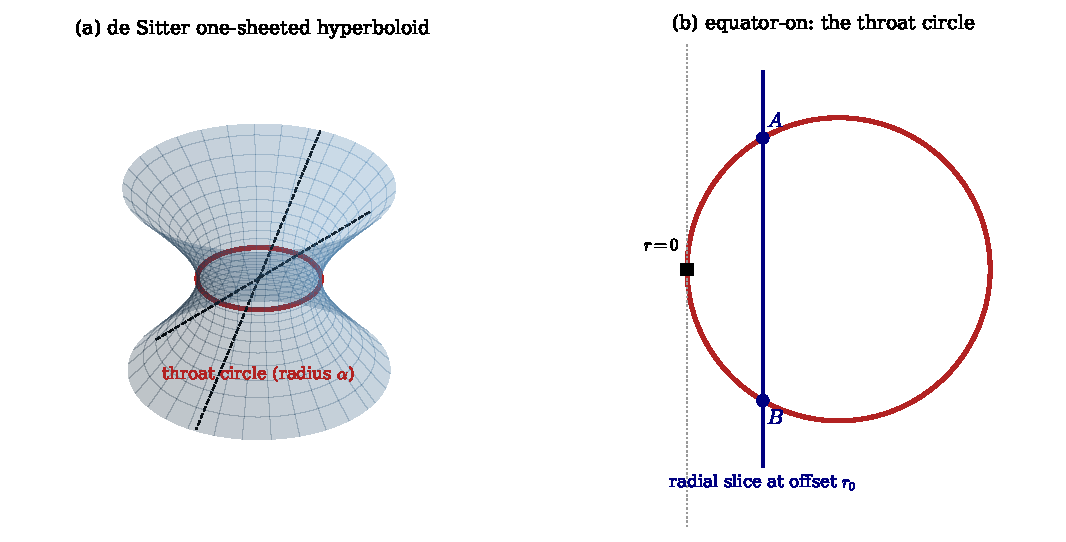
\includegraphics[width=\textwidth]{figs/fig2_throat_circle.pdf}
  \caption{(a) De Sitter space as the one-sheeted hyperboloid: finite at the
  equatorial throat, opening toward the poles, with asymptotic null structure
  shown dashed. (b) The equator-on view. The throat is a circle; the chart
  origin sits inside the hole, where the manifold is absent. A radial slicing
  line at offset $r_{0}$ meets the circle at two points, $A$ and $B$; the
  point $r=0$ is fixed at the back of the circle, diametrically opposite the
  hinge: a point \emph{on} the throat circle, at $X_{1}=-\alpha$. The whole
  equator carries embedding magnitude $X=\alpha$, so with the hinge at
  $X_{1}=+2\alpha$ (Section~\ref{sec:hinge-geometry}) the two stand $3\alpha$
  apart in the $X_{0}=0$ plane. The hinge fixes $r=0$; $A$ and $B$ move with
  the swing. Reconstructing the chart
  centre from the manifold requires traversing the whole ring.}
  \label{fig:throat}
\end{figure}

The cut itself is a single radial curve.

\begin{definition}[The slicing curve]\label{def:slicing}
The \emph{slicing curve} is the radial curve $r(l)$ defined by
\begin{equation}\label{eq:slicing}
  \frac{dr}{dl}=\sqrt{\lvert f(r)\rvert},
  \qquad
  f(r)=1-\frac{2M}{r}-\frac{r^{2}}{\alpha^{2}},
\end{equation}
where $l$ is proper distance along a radial slice, $dl=dr/\sqrt{\lvert f\rvert}$.
\end{definition}

The curve is the graph of the radial coordinate against proper radial distance. Its defining feature is immediate from \eqref{eq:slicing}: $dr/dl$ vanishes exactly where $f(r)=0$, that is, exactly at the horizons. The horizons are the turning points of the slicing curve. Proper distance $l$ enters here only as the integration variable that traces the curve; it is a derived quantity, demoted from the spine of the construction to the closing remark of Section~\ref{sec:remark}, for reasons that become visible at the Nariai configuration. The primary radial variable is $r$, signed (Section~\ref{sec:seam}); the primary parametrisation of the family is the swing angle of Section~\ref{sec:family}.

\section{Three parameters, and what each one flattens}\label{sec:params}

Three distinct quantities run through the construction, and letting them blur is what breeds confusion about it. We declare them once, with the structure each one is blind to, and use all three deliberately.

The first is the \emph{throat angle} $u$: position around the throat circle in the manifold, measured from $r=0$. It is a genuine geometric angle on a real circle of the geometry; a point of the unit throat circle at angle $u$ has chart coordinates $(\sin u,-\cos u)$. The second is the \emph{sky angle} $w$: the angular coordinate, on the charting observer's celestial sphere, of the line of sight relative to the centre of the hole's image (Section~\ref{sec:family}). It too is a genuine angle, but on a different surface---the sphere of directions at the observer's eye---and the gnomonic projection relates the two nonlinearly, $\sin u=\tfrac{2}{\sqrt3}\sin w$. The third is the \emph{signed areal radius} $r_{0}$: the areal value the slicing plane reads off at the designated seam, $r_{0}=\tfrac{2}{\sqrt3}\sin w$ along the real swing.

Each parameter flattens a different structure, and that is exactly why all three are needed. The throat angle $u$ is tied to one circle, so it is blind to which member of the family is in play and carries both harmonics of the horizon relation. The sky angle $w$ collapses the family's three-fold structure into the single $\sin 3w$ of the triple-angle relation, but in doing so folds the root-exchange involution $\sigma$ (the reflection $w\leftrightarrow\pi/3-w$) from view as a mere reflection. The signed radius $r_{0}$ is one number per seam, so it is blind to where on the conjugate lap one stands. Read together---the angle on the circle, the angle on the sky, the signed radius on the cut---they recover what each alone hides.

\section{The horizon structure, read in $r_{0}$}\label{sec:cubic}

A horizon is a zero of the metric function $f$. Clearing the denominator, in the gauge $\alpha=1$, gives the horizon cubic, and the turning-point structure of the slicing curve is read directly from it.

\begin{proposition}[Turning-point structure]\label{prop:turning}
The turning points of the slicing curve are the roots of the SdS horizon cubic. In the gauge $\alpha=1$,
\begin{equation}\label{eq:cubic}
  r\,f(r)=0
  \quad\Longleftrightarrow\quad
  r^{3}-r+2M=0 .
\end{equation}
At a simple root $r_{h}$ the turning point is non-degenerate, with
\begin{equation}
  \frac{d^{2}r}{dl^{2}}\Big|_{r_{h}}=\pm\tfrac12 f'(r_{h})\neq0;
\end{equation}
at a double root (Nariai~\cite{Nariai1951}) it is degenerate, $f'(r_{h})=0$.
\end{proposition}

\begin{proof}
Horizons are the zeros of $f$; multiplying $f(r)=1-2M/r-r^{2}$ by $r$ gives the cubic \eqref{eq:cubic}. Differentiating \eqref{eq:slicing}, $d^{2}r/dl^{2}=\tfrac{d}{dl}\sqrt{|f|}=(dr/dl)\,\tfrac{d}{dr}\sqrt{|f|}=\sqrt{|f|}\cdot\tfrac{f'}{2\sqrt{|f|}}\cdot\operatorname{sgn} f=\tfrac12 f'\operatorname{sgn} f$. At a simple root $f'(r_{h})\neq0$, so the second derivative is nonzero and the turning point is a genuine, non-degenerate extremum; at a double root $f'(r_{h})=0$ and it is degenerate.
\end{proof}

\emph{The proposition's own formula says what kind of system this is, and the potential it names was written down in the original derivation}~\cite[Eqs.~(4.24), Fig.~4.3]{JanzenThesis}: there $f$ is the scale-invariant \emph{effective potential} $V_{\mathrm{eff}}$ for a test particle, with $(\dd r/\dd\tau)^{2}=\gamma^{2}-V_{\mathrm{eff}}$ at vanishing angular momentum. Writing $V(r)=-\lvert f(r)\rvert/2$, the slicing law $(\dd r/\dd l)^{2}=\lvert f\rvert$ is $\tfrac12(\dd r/\dd l)^{2}+V(r)=0$ and the second derivative above is $-\dd V/\dd r$ exactly. \emph{So the slicing curve is the zero-energy orbit of a one-dimensional conservative system}, the horizon cubic is its turning-point condition $V=E$, and \emph{Nariai is the case where a turning point coincides with an equilibrium}: there $f$ has a double root, so $V$ and $V'$ vanish together and $V$ has a maximum at the orbit's own energy. \emph{That is why the degeneracy costs infinite affine parameter}---near an unstable equilibrium $\lvert f\rvert\simeq3(r-r_{N})^{2}$, so $\int\dd r/\sqrt{\lvert f\rvert}$ diverges logarithmically and the merged horizon is approached and never reached\ldg{integrable_systems}. \emph{And the vanishing surface gravity is the same statement}: $\kappa=f'(r_h)/2$ is $-V'(r_h)$, so $\kappa=0$ at Nariai \emph{is} the equilibrium condition, not a separate coincidence.

This is the precise sense in which the horizons \emph{are} turning points: the companion paper found the Schwarzschild horizon and singularity to be two non-degenerate critical points of the cycloid; Proposition~\ref{prop:turning} generalises that statement to the SdS family, with the cubic \eqref{eq:cubic} their defining equation.

\subsection{Factorisation with a root as parameter}

The construction becomes transparent the moment the slicing parameter is taken to be one of those roots. Write $2M=r_{0}-r_{0}^{3}$, which says exactly that $r_{0}$ is a root of \eqref{eq:cubic}.

\begin{proposition}[Factorisation]\label{prop:factor}
With $2M=r_{0}-r_{0}^{3}$, the horizon cubic factors as
\begin{equation}\label{eq:factored}
  r^{3}-r+2M=(r-r_{0})\bigl(r^{2}+r\,r_{0}+r_{0}^{2}-1\bigr)=0 .
\end{equation}
The three roots are $r_{0}$ and
\begin{equation}\label{eq:roots}
  r_{\mathrm{B}},\,r_{\mathrm{A}'}
  =\frac{-r_{0}\pm\sqrt{4-3r_{0}^{2}}}{2},
\end{equation}
and they sum to zero.
\end{proposition}

\begin{proof}
Since $2M=r_{0}-r_{0}^{3}$, the cubic is $r^{3}-r+r_{0}-r_{0}^{3}=(r^{3}-r_{0}^{3})-(r-r_{0})$. The first term factors as $(r-r_{0})(r^{2}+r r_{0}+r_{0}^{2})$ and the second contributes $-(r-r_{0})$, so the whole is $(r-r_{0})(r^{2}+r r_{0}+r_{0}^{2}-1)$. The quadratic factor has roots \eqref{eq:roots} by the quadratic formula. The sum of all three roots is the negated coefficient of $r^{2}$ in \eqref{eq:cubic}, which is zero.
\end{proof}

\begin{remark}[What the quadratic factor is]\label{rem:killing}
The conic $r^{2}+r\,r_{0}+r_{0}^{2}=1$ on which the cubic factors is not merely \emph{of} $A_{2}$ type; it is
the $A_{2}$ root hexagon's own circle, and identifying it costs nothing beyond putting two facts this
proposition already states side by side.\rcpt{P03_the_adjoint_is_entailed}\ldg{quadric_geometry} The roots sum to zero, so the root
triple lies in the plane $V=\{x\in\mathbb{R}^{3}:x_{1}+x_{2}+x_{3}=0\}$---which is the Cartan subalgebra of
$\mathfrak{su}(3)$ in its standard realisation, the diagonal traceless matrices. Parametrising $V$ by its first
two entries, $x=(a,b,-a-b)$, the induced Euclidean norm is
\[
  |x|^{2}=a^{2}+b^{2}+(a+b)^{2}=2\bigl(a^{2}+ab+b^{2}\bigr),
\]
\emph{exactly twice the quadratic factor of \eqref{eq:factored}}. So \eqref{eq:factored}'s conic is the unit
circle of the Killing form restricted to that Cartan. On it sit the six vectors $e_{i}-e_{j}$---which are this
construction's own designation transitions, the step to a neighbouring hinge whose reflections are the
involution $\sigma$ of Section~\ref{sec:cubic}---each of norm exactly $1$ in the form above, hence each lying
\emph{on} the conic. Those six satisfy the axioms of a reduced crystallographic root system in that form,
integrality included (the Cartan integers are $-2,-1,1,2$), with pairwise angles $0/60/120/180^{\circ}$ and no
right angle, and reflection group of order six. Since the reduced rank-two systems are exhausted by
$A_{1}\times A_{1}$, $A_{2}$, $B_{2}$ and $G_{2}$, with $4,6,8,12$ roots, six leaves only $A_{2}$.

\emph{What follows from that is a matter of record rather than of this paper}, and it is recorded because it
bears on a debt the programme carries elsewhere: a reduced irreducible root system determines a complex simple
Lie algebra uniquely, here $\mathfrak{sl}(3,\mathbb{C})$, of dimension $|\Phi|+\mathrm{rank}=6+2=8$---the
hexagon together with the sum-to-zero plane, counted---and the same root system fixes $|Z(\mathrm{SU}(3))|=3$ as
the determinant of its Cartan matrix. \emph{The centre and the adjoint are therefore one datum and not two.}
\emph{What this does not do is equally definite and is stated here rather than left to be inferred}: an algebra
being present is not a gauge symmetry being present. Nothing above supplies a bundle for it to act on, a
connection making the action gauged, or a reason matter should sit in the fundamental; the walls the companion
papers erect stand untouched, $\mathfrak{su}(3)$ being no subalgebra of $\mathfrak{so}(5,1)$ and the
$\mathfrak{su}(3)$ they place on the conjugate real form $S^{5}$ being reached by the global Wick rotation,
which the slicing never performs (Section~\ref{sec:seam})~\cite{JanzenBoundary,JanzenGeometricCore}. The debt
changes shape rather than size: what is owed is the object such an algebra would act on.
\end{remark}

The discriminant of the quadratic factor, $4-3r_{0}^{2}$, is the whole regime structure, read off $r_{0}$ and nothing else. It is positive for $|r_{0}|<2/\sqrt{3}$ (three distinct real roots, the undercritical regime), zero at $|r_{0}|=2/\sqrt{3}$ (a double root, Nariai), and negative for $|r_{0}|>2/\sqrt{3}$ (one real root and a complex-conjugate pair, the overcritical regime, Section~\ref{sec:overcritical}); the special value $r_{0}=1/\sqrt{3}$ makes $r_{0}$ itself coincide with $r_{\mathrm{B}}$, the Nariai case where two horizons merge. \emph{That quantity is the quadratic factor's discriminant in $r_{0}$, and it is worth distinguishing from the cubic's own, which is the root system's}: substituting $2M=r_{0}-r_{0}^{3}$ gives $\operatorname{disc}(r^{3}-r+2M)=(4-3r_{0}^{2})(3r_{0}^{2}-1)^{2}$, so the two differ by an exact square and their zero sets are \emph{not} the same. \emph{The squared factor is where the distinction earns its keep}: $4-3r_{0}^{2}$ vanishes at $r_{0}=\pm2/\sqrt3$, where the quadratic factor's own two roots collide, while the cubic's discriminant vanishes there \emph{and} at $r_{0}=\pm1/\sqrt3$, where the designated root $r_{0}$ collides with $r_{\mathrm{B}}$ instead. All four are Nariai---each carries $|2M|=2/(3\sqrt3)$ exactly and each leaves the cubic with a repeated root---so they are the four $r_{0}$-designations of the two Nariai configurations, and $4-3r_{0}^{2}$ sees only two of them. \emph{Which discriminant is meant therefore has to be said}, not because one set of zeros is not Nariai but because the slicing parameter's own discriminant misses half the designations at which it is reached. Restoring $\alpha$, the cubic's elementary symmetric functions are $e_{1}=0$, $e_{2}=-\alpha^{2}$ and $e_{3}=-2M\alpha^{2}$: $e_{1}=0$ is the tracelessness that puts the roots in the Cartan at all, and the other two are the $A_{2}$ Weyl group's two basic invariants, of degrees two and three---the degrees of $\mathfrak{su}(3)$'s two Casimirs\ldg{representation_theory}. \emph{So the slicing's two parameters are not two numbers the construction happens to carry but the complete invariant content of the $A_{2}$ it already realises}; and since \emph{that} discriminant, $-4e_{2}^{3}-27e_{3}^{2}$, is the Weyl invariant vanishing where two roots collide, \emph{Nariai is the wall of the Weyl chamber and the undercritical dial its interior}. This is the point of reading in $r_{0}$: the three regimes are fixed by a single algebraic quantity, with no appeal to a proper distance diverging and no ``two limits of one object.'' Nariai is not a pathology reached by something blowing up; it is the value of $r_{0}$ at which the discriminant vanishes. The three roots sum to zero, so they cannot share a sign: in the undercritical regime they are two of one sign and one of the other. For $2M>0$ the cubic has two positive roots and one negative; for $2M<0$, one positive and two negative; the negative-root horizon of the first case is the backward-radial root carried by the major axis of the locus ellipse (Section~\ref{sec:ellipse}).

\subsection{The reading-swap as a symmetry of the line element}\label{sec:reading}

\begin{proposition}\label{prop:r0zero}
At $r_{0}=0$ the metric function is $f=1-r^{2}$, which is pure de Sitter; the cubic's roots there are $\{0,+1,-1\}$. This single parameter value carries two readings of one slicing---the de Sitter reading directly, and the Schwarzschild reading by the backward-radial vantage-swap---the full account of which is given at the throat in Section~\ref{sec:family}.
\end{proposition}

\begin{proof}
From \eqref{eq:sds} in the gauge $\alpha=1$, $f=1-2M/r-r^{2}=-(r-r_{0})(r^{2}+r r_{0}+r_{0}^{2}-1)/r$ by Proposition~\ref{prop:factor}. At $r_{0}=0$ this is $-(r)(r^{2}-1)/r=-(r^{2}-1)=1-r^{2}$, the de Sitter metric function. And $2M=r_{0}-r_{0}^{3}=0$ at $r_{0}=0$. The roots of $r^{3}-r=0$ are $0,\pm1$.
\end{proof}

The reading-swap is not confined to $r_{0}=0$. It is, for every slicing parameter, a symmetry of the line element itself.

\begin{proposition}[The reading-swap is a line-element symmetry]\label{prop:readingswap}
For every $r_{0}$, designating $r_{\mathrm{B}}$ rather than $r_{0}$ as the slicing parameter leaves the metric function $f$ unchanged. Equivalently, the mass parameter is invariant under the root-exchange involution,
\begin{equation}
  2M(r_{\mathrm{B}})=2M(r_{0}).
\end{equation}
\end{proposition}

\begin{proof}
By construction $2M=r_{0}-r_{0}^{3}$, the statement that $r_{0}$ is a root of $r^{3}-r+2M=0$. By Proposition~\ref{prop:factor}, $r_{\mathrm{B}}$ is also a root of that same cubic, so $r_{\mathrm{B}}^{3}-r_{\mathrm{B}}+2M=0$, i.e. $2M=r_{\mathrm{B}}-r_{\mathrm{B}}^{3}$. Hence $r_{0}-r_{0}^{3}=r_{\mathrm{B}}-r_{\mathrm{B}}^{3}$: the mass parameter is the same whichever of the two positive roots is taken as the slicing parameter. Since $f(r)=1-2M/r-r^{2}/\alpha^{2}$ depends on $r_{0}$ only through $2M$, the metric function is identical under the exchange.
\end{proof}

The reading-swap is therefore a genuine symmetry of the SdS line element, not a coincidence at one point: the involution exchanges which root is designated the mass-horizon while leaving the geometry strictly unchanged. The two readings are two designations within one line element---and they separate into the two \emph{named} geometries, de Sitter and Schwarzschild, only as the two causal vantages at the throat (Section~\ref{sec:family}), the throat radius $\alpha$ left fixed throughout. \emph{A second partition of the same triple runs alongside the designation, and the two are neither independent nor identical.}\rcpt{P03_the_two_splits} From the factorisation above the designated root is $r_{0}$ and the pair is $(-r_{0}\pm\sqrt{4-3r_{0}^{2}})/2$, whose product is $r_{0}^{2}-1$; so the pair members share a sign---and the designation split therefore coincides with the split by \emph{sign} of the roots---exactly when $|r_{0}|>1$, and differ otherwise. The discriminating quantity is the offset and not the mass, and the boundary $|r_{0}|=1$ is the $M=0$ member, the de~Sitter one. At Nariai the two do not merely differ: the designated root there merges with a pair member, so the designation split loses its content while the sign split stays sharp. \emph{Two structures that fail in different places are not two readings of one structure}, which is the reason for stating the relation rather than leaving the two partitions side by side. Reading this symmetry in $r_{0}$ is what exhibits it as a literal symmetry of the line element; reading it in the sky angle (Section~\ref{sec:family}) folds it from view as a mere reflection.

\subsection{The involution}

\begin{proposition}[The root-exchange involution]\label{prop:involution}
The map
\begin{equation}\label{eq:involution}
  \sigma(r_{0})=\frac{-r_{0}+\sqrt{4-3r_{0}^{2}}}{2}
\end{equation}
is an involution: $\sigma(\sigma(r_{0}))=r_{0}$ on $[0,2/\sqrt{3}]$. It carries the slicing parameter to the second positive root of its own cubic, fixes $r_{0}=1/\sqrt{3}$ (Nariai, the designated root sitting on the merged pair), and exchanges the endpoints, $\sigma(0)=1$ and $\sigma(1)=0$.
\end{proposition}

\begin{proof}
Equation \eqref{eq:involution} is $r_{\mathrm{B}}$ of \eqref{eq:roots} read as a function of the parameter $r_{0}$. Write $s=\sqrt{4-3r_{0}^{2}}$, so $\sigma(r_{0})=(-r_{0}+s)/2$. Then
\[
  4-3\sigma(r_{0})^{2}
  =4-\tfrac34(-r_{0}+s)^{2}
  =4-\tfrac34\bigl(r_{0}^{2}-2r_{0}s+s^{2}\bigr).
\]
Substituting $s^{2}=4-3r_{0}^{2}$ and simplifying gives the perfect square
\[
  4-3\sigma(r_{0})^{2}=\Bigl(\tfrac{3r_{0}+s}{2}\Bigr)^{2},
  \qquad\text{hence}\qquad
  \sqrt{4-3\sigma(r_{0})^{2}}=\frac{3r_{0}+s}{2}
\]
on the positive branch. Therefore
\[
  \sigma(\sigma(r_{0}))
  =\frac{-\sigma(r_{0})+\sqrt{4-3\sigma(r_{0})^{2}}}{2}
  =\frac{-\tfrac12(-r_{0}+s)+\tfrac12(3r_{0}+s)}{2}
  =\frac{\tfrac12(4r_{0})}{2}
  =r_{0}.
\]
The fixed point solves $\sigma(r_{0})=r_{0}$, i.e. $-r_{0}+\sqrt{4-3r_{0}^{2}}=2r_{0}$, so $\sqrt{4-3r_{0}^{2}}=3r_{0}$, $4-3r_{0}^{2}=9r_{0}^{2}$, $r_{0}=1/\sqrt3$. The endpoint values are $\sigma(0)=\sqrt4/2=1$ and $\sigma(1)=(-1+1)/2=0$.
\end{proof}

\begin{remark}
The three roots of the cubic are interchangeable labels, and \eqref{eq:involution} is the explicit map that swaps the two non-negative roots while leaving the third fixed. It acts \emph{within} the positive-root half ($r_{0}\in[0,2/\sqrt3]$, $2M\ge0$): the negative-root half ($2M<0$, two negative roots) is reached not by $\sigma$ but by the backward-radial reflection $(r_{0},r)\mapsto(-r_{0},-r)$ of Section~\ref{sec:ellipse}---the outer $\mathbb{Z}_{2}$ ($2M\mapsto-2M$) which with $\sigma$ and the sky-angle periodicity generates the full discrete symmetry $\mathrm{Aut}(A_{2})=S_{3}\times\mathbb{Z}_{2}\cong D_{6}$ (Proposition~\ref{prop:morphism-generation}). $\sigma$ is thus one generator restricted to a sign-half, not the general action; the reflection through the origin is its locked-in complement. The de Sitter configuration ($r_{0}=0$) and the chart-tangent configuration ($r_{0}=1$, where the slicing line meets the throat at a single point) are exchanged by the involution; its fixed point is Nariai, where the two positive roots coincide. The same Nariai geometry is met at $|r_{0}|=2/\sqrt3$ with the lone root designated and the other two merging: one geometry under two designations, which is the content of the involution. This is the general rule, not a feature of Nariai alone: $r_{0}$ is a value of the areal radius and the cubic is many-to-one, so each geometry is met at several $r_{0}$-values---one per root it may designate---while the swing angle $w$ places each geometry \emph{once} (Section~\ref{sec:family}). The several $r_{0}$-values are designations of the areal radius at one dial angle, not several angles; reading them as several positions on the dial mistakes the areal radius for the angle. Figure~\ref{fig:cubic} shows the cubic and the involution. Two partitions of the same three roots are in play here and they are not the same partition: the designated root stands against the pair on the conic, while the roots also divide by sign, and the conic pair generally carries one root of each sign, so the designated root is not in general the odd one by sign. The two differ in kind as well as in extension. Holding the geometry fixed and cycling the designation through all three roots leaves the sign division untouched, so that one is a property of the geometry while the designation is a property of the vantage---the same division the construction draws between what is on the throat circle and what is tangent to it, appearing here inside a single triple\rcpt{P03_two_two_plus_ones}. At the degenerate member they meet: with the lone root designated it is also the odd one by sign, which is a second reading of the one geometry met under two designations.
\end{remark}

\begin{figure}[t]
  \centering
  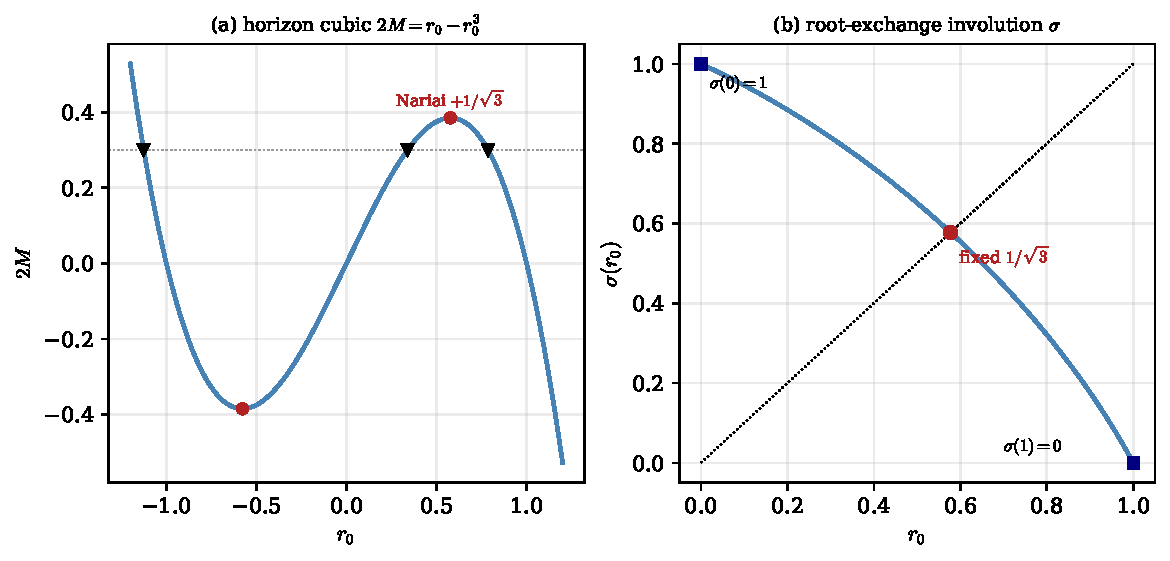
\includegraphics[width=\textwidth]{figs/fig3_cubic_involution.pdf}
  \caption{(a) The horizon cubic in the form $2M=r_{0}-r_{0}^{3}$. A given
  value of $2M$ is met by three roots (three horizons); the triplet is the
  content of the factorisation \eqref{eq:factored}. The marked extrema at
  $r_{0}=\pm1/\sqrt{3}$ are the Nariai double-root locus.
  (b) The root-exchange involution $\sigma(r_{0})=\tfrac12(-r_{0}+\sqrt{4-3r_{0}^{2}})$,
  with $\sigma(\sigma(r_{0}))=r_{0}$. It exchanges the endpoints $0\leftrightarrow1$ and
  fixes $r_{0}=1/\sqrt{3}$, the Nariai configuration.}
  \label{fig:cubic}
\end{figure}

\subsection{The horizon locus: a line and a tilted ellipse}\label{sec:ellipse}

Taken over all values of the slicing parameter at once, the horizon triplet traces a definite locus in the $(r_{0},r)$-plane.

\begin{proposition}[The horizon locus]\label{prop:locus}\ldg{algebraic_geometry}
In the $(r_{0},r)$-plane the horizon locus---the set of $(r_{0},r)$ for which $r$ is a horizon of the geometry with slicing parameter $r_{0}$---is
\begin{equation}
  g(r)=g(r_{0}),\qquad g(t)=t^{3}-t,
\end{equation}
and it factors into a straight line and a conic,
\begin{equation}\label{eq:locusfactor}
  (r-r_{0})\,\bigl(r^{2}+r\,r_{0}+r_{0}^{2}-1\bigr)=0 .
\end{equation}
The conic $r^{2}+r\,r_{0}+r_{0}^{2}=1$ is an ellipse whose major axis lies along the anti-diagonal $r=-r_{0}$; it is tilted at $45^{\circ}$---the \emph{fundamental ellipse} of~\cite[Fig.~4.2]{JanzenThesis}, where the $(r,r_{0})$-plane carrying it was first drawn. \emph{The conic itself is not new here}: it is Eq.~(SdS\_ellipse) of the 2012 dissertation, obtained there directly from the scale-invariant line element, together with the horizon equation $r^{3}-r_{0}^{3}-(r-r_{0})=0$ it factors and the explicit pair of further horizons $r=-\tfrac{r_{0}}2\pm\tfrac12\sqrt{4-3r_{0}^{2}}$~\cite[Eqs.~(4.10)--(4.12)]{JanzenThesis}. \emph{What is added here is the reading}: that the locus factors as a line and a conic, that the tilt is $45^{\circ}$, and that the two components meet at Nariai.\rcpt{P03_cubic_factor_ellipse_locus}
\end{proposition}

\begin{proof}
A horizon of the geometry with parameter $r_{0}$ is a root $r$ of $r^{3}-r+2M=0$ with $2M=r_{0}-r_{0}^{3}$; thus $r^{3}-r=r_{0}^{3}-r_{0}$, i.e. $g(r)=g(r_{0})$. The difference $g(r)-g(r_{0})=(r^{3}-r_{0}^{3})-(r-r_{0})$ factors as $(r-r_{0})(r^{2}+r r_{0}+r_{0}^{2}-1)$, which is \eqref{eq:locusfactor}. The quadratic form $r^{2}+r r_{0}+r_{0}^{2}$ has matrix $\bigl(\begin{smallmatrix}1&1/2\\1/2&1\end{smallmatrix}\bigr)$, with eigenvalues $1/2$ and $3/2$ and eigenvectors $(1,1)$ and $(1,-1)$. Both eigenvalues are positive, so the conic is an ellipse; the smaller eigenvalue $1/2$ belongs to the eigenvector $(1,-1)$, giving the longer semi-axis $\sqrt{2}$ along the anti-diagonal $r=-r_{0}$, and the larger eigenvalue $3/2$ the shorter semi-axis $\sqrt{2/3}$ along the diagonal $r=r_{0}$.
\end{proof}

\begin{corollary}[Nariai is where the locus's two components meet]\label{cor:nariai-locus}
The line and the conic of Proposition~\ref{prop:locus} meet exactly at the two Nariai
configurations. Substituting $r=r_{0}$ into the conic gives $3r_{0}^{2}=1$, so the
intersections are $r_{0}=\pm1/\sqrt3$, at which the cubic acquires its double root---the
merged horizon---and the third root sits at $\mp2/\sqrt3$. Equivalently, since the line
$r=r_{0}$ is the diagonal along which the conic's shorter semi-axis $\sqrt{2/3}$ lies, the two
Nariai configurations are the endpoints of the fundamental ellipse's minor
axis, $\sqrt{2/3}\,(1,1)/\sqrt2=(1/\sqrt3,1/\sqrt3)$.\rcpt{Q5_nariai_on_the_locus}
\end{corollary}

\begin{remark}
The corollary adds no new value; it locates one already fixed three ways. Nariai is
\emph{algebraically} the cubic's double root and the fixed point of the root-exchange
$\sigma$ (Proposition~\ref{prop:involution}); it is \emph{incidence-geometrically} the singular
point of the reducible cubic $g(r)=g(r_{0})$, where its line component meets its conic; and it
is \emph{metrically} the end of that conic's minor axis. That the degenerate configuration of
the family is the singular point of the family's own locus is the geometric content the
algebraic statement carries without displaying.
\end{remark}

The line $r=r_{0}$ is the trivial root---the slicing parameter is always itself a horizon---and the ellipse carries the other two (Figure~\ref{fig:ellipse}). The anti-diagonal is the geometrically meaningful axis: the ellipse is symmetric under $(r_{0},r)\mapsto(-r_{0},-r)$, the reflection through the origin which is the exchange $r\to-r$, the \emph{backward radial direction}---the radial coordinate run in the negative sense, the long way from $r=0$. The negative root of the horizon cubic, which appears whenever the other two roots are positive, is not a bookkeeping artefact and not unphysical: it is the horizon reached in the backward radial direction. The companion paper already carried this, the continuation $z\mapsto\pi+i\rho'$ at the conjugate critical point of the cycloid producing the back-seam continuation onto $r<0$; the major axis of the tilted ellipse is the locus of that backward direction. The reflection $(r_{0},r)\mapsto(r,r_{0})$ across the diagonal, by contrast, is the relabelling of which root is called the parameter---the root-exchange involution of Proposition~\ref{prop:involution} seen in the plane.

\begin{figure}[t]
  \centering
  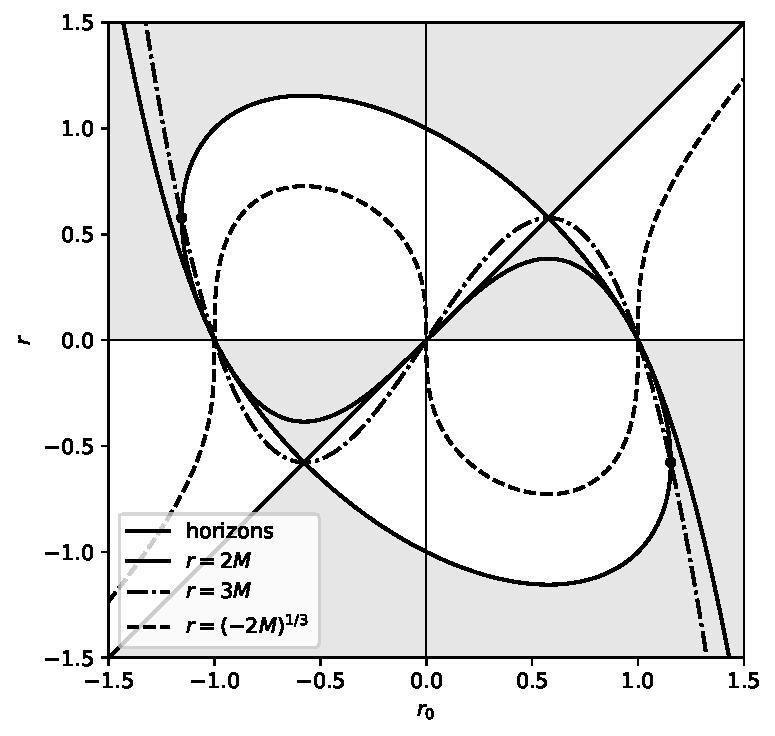
\includegraphics[width=0.62\textwidth]{figs/fig6_tilted_ellipse.pdf}
  \caption{The horizon locus $g(r)=g(r_{0})$: the diagonal line $r=r_{0}$ (the
  trivial root) and the $45^{\circ}$ tilted ellipse $r^{2}+r r_{0}+r_{0}^{2}=1$
  (the other two roots), drawn dotted. A vertical line at fixed $r_{0}$ meets the
  locus in three horizons. The ellipse's major axis is the anti-diagonal
  $r=-r_{0}$, the backward radial direction; its minor axis is the diagonal
  $r=r_{0}$. The marked vertical-tangent points are the Nariai configurations,
  where two horizons merge; the same Nariai geometry is met on the diagonal at
  $r_{0}=r=1/\sqrt{3}$, with the lone root designated instead.
  The figure is a map of the whole family at once---every point $(r_{0},r)$ is a
  radius in the geometry that $r_{0}$ slices---and the shading is the sign of
  $f$: grey where $f<0$, inside a horizon, where the radial direction is
  timelike and the cut reads as an expanding cosmology (Section~\ref{sec:family}).
  Carried with it are the Schwarzschild radius $r=2M$ and the photon sphere
  $r=3M$ across the family---and the photon sphere meets the horizon locus exactly at Nariai, which is worth stating rather than leaving to the eye. The photon sphere solves $\dd(f/r^{2})/\dd r=0$, giving $r=3M$ independently of $\alpha$; at the Nariai value $M=\alpha/3\sqrt3$ that is $r=\alpha/\sqrt3$, the merged double root, where $f=f'=0$\rcpt{O1_photon_sphere_nariai}. The framework paper forces the same member by a trichotomy on how the reassigned null congruence meets the horizon---transverse, tangent at the merged root, or no horizon~\cite{JanzenCRframework}---and a null direction tangent to a sphere of constant $r$ is a circular null orbit, so the two conditions are one condition reached twice. What the optical reading adds is that the forced member's photon sphere is null-degenerate: sitting on the horizon, its impact parameter $b^{2}=r^{2}/f$ diverges, and the comoving turnaround $r=(-2M)^{1/3}$---the
  root of the \emph{other} cubic $r^{3}=-2M\alpha^{2}$, where the $E{=}1$
  congruence turns, as against the horizons $f=0$ where the slicing turns. The
  two loci appear together here and are affinely inequivalent; that no affine
  change of variable identifies their two threefold symmetries---the two cubics
  being the $E{=}1$ and $E{=}0$ ends of one family of turning points---is the
  companion framework paper's \emph{lem:twoturnings} and its remark. Read off the Nariai ordinate,
  however, the merged horizon $r_{N}=\alpha/\sqrt{3}$ and the turnaround
  $A_r=(2M\alpha^{2})^{1/3}$ stand in the ratio $A_r=\sqrt[3]{2}\,r_{N}$, both falling
  out of the one double-root factorisation
  $(r-r_{N})^{2}(r+2r_{N})=r^{3}-3r_{N}^{2}r+2r_{N}^{3}$---a ratio between two radii,
  which the lemma does not touch. (Janzen 2012, Fig.~4.3.)}
  \label{fig:ellipse}
\end{figure}

The Nariai configurations are the vertical-tangent points of the ellipse, at $r_{0}=\pm2/\sqrt{3}$ with $r=\mp1/\sqrt{3}$: there two horizons of the triplet merge. For $|r_{0}|<2/\sqrt{3}$ the vertical line at $r_{0}$ meets the ellipse in two real points and the locus in three real horizons; for $|r_{0}|>2/\sqrt{3}$ it misses the ellipse and only the diagonal root is real. The single threshold $|r_{0}|=2/\sqrt{3}$, equivalently $|2M|=2/(3\sqrt{3})$, is the undercritical/overcritical boundary, treated in Section~\ref{sec:overcritical}.

The ellipse carries, beyond its three roots, two distinguished points of its own: its foci\rcpt{P03_ellipse_foci}\ldg{spectral_theory}. With semi-axes $\sqrt2$ and $\sqrt{2/3}$ the focal distance is $c=\sqrt{a^{2}-b^{2}}=\sqrt{2-2/3}=2/\sqrt3$, so the foci lie on the backward-radial major axis at the value $2/\sqrt3$---the Nariai offset, the extreme $r_{0}$ of the ellipse, which is the lone backward-radial root the closed slicing runs out onto and closes on (Section~\ref{sec:lap}). This is not a coincidence of the number. The axis ratio is $a/b=\sqrt3$---the equilateral signature carried by the unit cross-term---and for that ratio alone the focal distance $\sqrt{a^{2}-b^{2}}$ equals the $r_{0}$-half-width $\sqrt{(a^{2}+b^{2})/2}$, which is the Nariai offset; so the metric foci of the horizon locus and the root the curve closes on stand at one scale, the forced $2/\sqrt3=2\alpha/\sqrt3=2/\sqrt\Lambda$, twice the merged-pair radius $\alpha/\sqrt3$. In the sky angle (Section~\ref{sec:throat-angle}) the foci fall at $w=\pi/4$, the exact bisector of the Nariai crest $w=\pi/6$ and the throat-tangent extreme $w=\pi/3$ at which the rulings touch---all three carried on the one gnomonic sweep $r_{0}=\tfrac2{\sqrt3}\sin w$. \emph{One qualification belongs with the word ``metric'', and it protects the reading rather than weakening it.}\rcpt{P03_the_foci_are_chart_objects} A focus is not a projective invariant of a conic: it is defined against a metric, and the metric used here is the $(r,r_{0})$ chart's Euclidean one, the two axes at equal scale and at right angles. Read instead with the $A_{2}$ form \emph{itself} as the metric, the locus $Q=1$ is by definition that form's unit sphere---a circle, of eccentricity zero, whose foci coincide at the centre. That the two readings genuinely differ is visible in the Weyl action: the three-cycle $(r_{1},r_{2})\mapsto(r_{2},-r_{1}-r_{2})$ preserves the form and is \emph{not} orthogonal in the chart, so the locus is Weyl-invariant as a set while the Weyl action is not by chart-rotations. \emph{What is chart-dependent is that the consequence presents itself as a pair of points; the number is not.} The focal distance is $\sqrt{a^{2}-b^{2}}$ with the axis ratio fixed at $\sqrt3$ by the unit cross-term, so $2/\sqrt3$ is a consequence of the form and stands however the locus is drawn---which is why the statement made here is a statement about one \emph{scale} carrying several structures, and not an identification of the foci with any object of the embedding.

\section{The family in $w$, and the two readings at the throat}\label{sec:family}

The slicing plane swings about the hinge (Section~\ref{sec:slicing}), and the swing angle $w$ is the family parameter---the same angle the gnomonic projection below reads as the observer's sky angle. At each $w>0$ the cut takes three horizons: the cosmological horizon, the black-hole horizon standing above $r=0$, and $r=0$ itself fixed at the back of the circle. The mass is nonzero and is the slicing-dependent factor, $2M=\alpha[(r_{0}/\alpha)-(r_{0}/\alpha)^{3}]$, with $\alpha=\sqrt{3/\Lambda}$ the one fixed invariant---never a free parameter, never reached by a limit (Section~\ref{sec:mass}).

\subsection{The projection is the observer's celestial sphere}\label{sec:projection}

It remains to say where the offset $r_{0}$ comes from. It is not a free parameter dialled by hand; it is fixed by what an observer in the manifold can actually see, and the act of fixing it is the symmetry breaking itself.

Consider an observer in the exterior, at finite distance from the hole. The hole has exact rotational symmetry about its own centre; the observer, sitting at one point of the exterior, does not share that symmetry---they are at a definite radius from the centre, along a definite direction. There are then two distinct radial lines in play, and they must not be conflated. One is the \emph{hole-radial}: the line from the centre of the hole to the observer, the line the hole's own symmetry would single out. The other is the observer's \emph{line of sight}: the direction the observer takes to be straight ahead.

The observer cannot see the hole's centre. What an observer in the manifold has is the image of the hole on their \emph{celestial sphere}---the unit sphere of directions at their eye. The hole's outline is a small circle of some angular radius on that sphere; the observer cannot see around it or locate its true centre by inspection; the sky image is all they have. The observer fixes their frame on what they can see: they place the centre of their field of view---their reticle---on the sky image. If they place it on the image's apparent centre, the line of sight coincides with the hole-radial and there is no offset. But there is no reason the reticle should land there: the apparent centre of a projected image is not a marked point, and any other choice places the reticle off-centre. The moment the reticle sits off the image's centre, the line of sight and the hole-radial part company.

This is the symmetry breaking, located precisely. The manifold's one broken symmetry is the hole. An observer who takes the hole as reference is then forced to break a further symmetry---not by choice, but because their reference is a sky image and the reticle on it is off-centre. Two roles are in play here and will be separated sharply in Section~\ref{sec:groupoid}: the \emph{manifold observer}, whose physical position in the exterior fixes the offset $r_{0}$ as an intrinsic feature of the slicing curve, and the \emph{charting observer}, whose celestial-sphere image merely displays that offset. Moving the charting observer changes the image, never $r_{0}$.

The chart is not a flat Cartesian plane: the hole's image lives on the curved celestial sphere, and to obtain a planar chart the sphere must be projected. The projection is forced---not chosen---by the construction, and it is the \emph{gnomonic} projection~\cite{Snyder1987}.

\begin{proposition}[The projection is gnomonic]\label{prop:gnomonic}
The planar chart of the throat is the gnomonic projection of the observer's celestial sphere from its centre. The orthographic projection is excluded.
\end{proposition}

\begin{proof}
The observer's line of sight is a straight radial line, and a faithful planar chart must carry it to a straight line. The gnomonic projection---from the sphere's centre---is the unique projection that sends every great circle to a straight line, so the straight line of sight remains a straight slicing line in the chart. It is forced by this straight-line geometry alone, independently of the observer or the slicing scale; the orthographic projection, lacking this property, is thereby excluded. The same criterion excludes the stereographic projection, and it is worth naming which criterion that is: the stereographic is the \emph{conformal} projection of the sphere, preserving angles, and it carries great circles to circles rather than to lines\rcpt{C4_gnomonic_not_conformal}\ldg{conformal_geometry}. The chart this construction requires is therefore the one that preserves straightness at the cost of angles, not the one that preserves angles at the cost of straightness---a projective demand rather than a conformal one, which is the character of the construction throughout---and the standing consequence is worth saying once rather than leaving to be inferred: \emph{this construction is not conformally invariant, and does not want to be}. A conformally invariant reading would keep the angles and lose the straight line of sight, which is the one thing the slicing is built on. The causal structure it inherits is conformal, as any causal structure is; the construction erected over that structure is projective, and the scale $\alpha$ is precisely what the conformal reading does not fix and the projective one does\ldg{conformal_geometry}. The distinguished scale confirms the same exclusion. For the horizon relation to linearise to a single triple-angle in the sky angle (Proposition~\ref{prop:triple}) the throat's planar image must have radius $R=2/\sqrt3$; a small circle of angular radius $\theta$ on the unit sphere has planar radius $\sin\theta$ under orthographic projection and $\tan\theta$ under gnomonic, so the orthographic image---bounded by $\sin\theta\le1$---can never reach $2/\sqrt3>1$, whereas the gnomonic radius $\tan\theta=2/\sqrt3$ has the real solution $\theta=\arctan(2/\sqrt3)$.
\end{proof}

Place the observer in the equatorial plane at distance $r_{\mathrm{obs}}$ from the hole's centre, with the throat circle of unit radius (gauge $\alpha=1$). The throat subtends true angular radius $\theta=\arcsin(1/r_{\mathrm{obs}})$ on the observer's celestial sphere---the tangent half-angle of the unit throat at distance $r_{\mathrm{obs}}$---with gnomonic image radius $\tan\theta=1/\sqrt{r_{\mathrm{obs}}^{2}-1}$. A line of sight at sky-angle $w$ from the image-centre meets the throat's image at offset
\begin{equation}\label{eq:x0proj}
  r_{0}=\frac{2}{\sqrt3}\,\sin w ,
\end{equation}
the image radius $2/\sqrt3$ times the sine of the genuine sky angle. This image radius is not an observer's free choice: it is \emph{forced} to $2/\sqrt3$ by the requirement that the horizon relation linearise to the pure triple-angle (Proposition~\ref{prop:triple}), the unique scale that removes the residual harmonic. The charting distance realising it is $r_{\mathrm{obs}}=\sqrt7/2$ (where $1/\sqrt{r_{\mathrm{obs}}^{2}-1}=2/\sqrt3$); but the scale is set by the triple-angle, not by placing an observer, and any other charting distance only rescales $w$ without touching the geometry---though not without cost to the form: the residual $\sin w$ harmonic that Proposition~\ref{prop:triple} removes returns at every other value\rcpt{O3_charting_distance}, so $r_{\mathrm{obs}}=\sqrt7/2$ is the distance at which the family's own harmonic structure is legible rather than a place an observer happens to stand.

\subsection{The sky angle, the triple-angle, and the conjugacy}\label{sec:throat-angle}

Let $w$ be the sky angle of \eqref{eq:x0proj}. By \eqref{eq:x0proj} the slicing line meets the throat's gnomonic image at offset
\begin{equation}\label{eq:x0sinw}
  r_{0}=\frac{2}{\sqrt3}\,\sin w ,
\end{equation}
an exact geometric identification: $w$ is a genuine angle on the celestial sphere, and $r_{0}$ is the throat-image radius $2/\sqrt3$ times its sine. The chart range $r_{0}\in[0,1]$ is $w\in[0,\pi/3]$, the throat-tangent extreme $r_{0}=1$ being $w=\pi/3$.

\begin{proposition}[The horizon relation in the sky angle]\label{prop:triple}
With $r_{0}=\tfrac{2}{\sqrt3}\sin w$, the horizon relation $2M=r_{0}-r_{0}^{3}$ is the pure triple-angle relation
\begin{equation}\label{eq:tripleM}
  2M=\frac{2}{3\sqrt3}\,\sin(3w),
\end{equation}
and the image radius $2/\sqrt3$ is the unique value of the slicing scale for which this holds.\rcpt{P03_triple_angle_gnomonic}
\end{proposition}

\begin{proof}
With $r_{0}=\varrho\sin w$, expand $r_{0}-r_{0}^{3}=\varrho\sin w-\varrho^{3}\sin^{3}w$. Using $\sin^{3}w=\tfrac14(3\sin w-\sin 3w)$,
\[
  r_{0}-r_{0}^{3}=\Bigl(\varrho-\tfrac34 \varrho^{3}\Bigr)\sin w+\tfrac14 \varrho^{3}\sin 3w .
\]
The relation is a pure multiple of $\sin 3w$---with no residual $\sin w$ harmonic---if and only if $\varrho-\tfrac34 \varrho^{3}=0$, whose unique positive root is $\varrho=2/\sqrt3$\ldg{harmonic_analysis}. At that value $\tfrac14 \varrho^{3}=2/(3\sqrt3)$, giving \eqref{eq:tripleM}.
\end{proof}

This is why a cubic appears, and why the sky angle is its natural coordinate: the cubic $r_{0}-r_{0}^{3}$ is the cubic in $\sin w$ that the triple-angle identity collapses to $\sin 3w$, and the slicing scale $2/\sqrt3$ is the one scale removing the residual harmonic. The three roots of the horizon cubic are the three preimages $w,\ \tfrac{\pi}{3}-w,\ -\tfrac{\pi}{3}-w$ of $3w$ under the sine. The involution \eqref{eq:involution} is, in the sky angle, the reflection $w\leftrightarrow\tfrac{\pi}{3}-w$, a symmetry of $\sin 3w$ because $\sin\!\bigl(3(\tfrac{\pi}{3}-w)\bigr)=\sin(\pi-3w)=\sin 3w$; its fixed point $w=\pi/6$ is the crest of $\sin 3w$, which is why Nariai is a double root. A further shift makes the cyclic structure explicit: since $\sin 3w$ is unchanged under $w\mapsto w+2\pi/3$, three sky angles $120^\circ$ apart carry the \emph{same} mass while cycling which root is the designated offset through all three---the cyclic $\mathbb{Z}_3$ within $S_3$, $\sigma$ (the $\pi/3$-reflection) supplying the transposition. These are three $120^\circ$-separated hinged vantages of the one sliced substrate, each designating one root: the monodromy three-fold read as three readings of the one geometry (its group-theoretic form in~\cite{JanzenGroupoid}). Read on a fermion sector this three-fold is the generation multiplicity---forced to three by the single triple-angle at the gnomonic-fixed scale, not fitted, the three hinged vantages an $S_3$---a \emph{within-state} index rather than a family symmetry, the generations' own threeness being the turnaround's deck $\mathbb{Z}_3$ since the revision the matter sector made and this paper follows---and the wall structure fixing the \emph{number} of chiral generations at either seat on the matter sector~\cite{JanzenMatter}, forced within CR; the continuous $\mathrm{SU}(3)$ that shares the root system, not an isometry of the Lorentzian substrate, is placed on its conjugate real form ($S^{5}=\mathrm{SO}(6)/\mathrm{SO}(5)$) in the boundary and geometric-core papers, with only its identification as the physical colour left
open~\cite{JanzenBoundary,JanzenGeometricCore}.

\begin{remark}[The triple angle is available in four spacetime dimensions and, with a caveat, in five; in no other]\label{rem:dimension}
Proposition~\ref{prop:triple} is a statement about a cubic, and it is worth asking what the same demand returns
in other dimensions, because the answer is narrow. In $D$-dimensional Schwarzschild--de~Sitter the metric
function is $f=1-2M/r^{D-3}-r^{2}/\alpha^{2}$, so in the gauge $\alpha=1$ the mass is the slicing-dependent
factor $2M=r_{0}^{D-3}-r_{0}^{D-1}$. Substituting $r_{0}=\varrho\sin w$ as above and expanding in the
multiple-angle basis, the harmonics present are $\sin$ or $\cos$ of $(D-1)w,\,(D-3)w,\ldots$, so the number
standing \emph{below} the top one is exactly one at $D=4$ and $D=5$ and two or more from $D=6$ upward---while
the construction has exactly one scale $\varrho$ to spend. Hence no slicing scale removes the residual
harmonics from six dimensions up: there is no pure multiple-angle, the $D-1$ dial positions spaced
$2\pi/(D-1)$ apart no longer carry a common mass, and the family has no forced fold to read. At $D=5$ the
collapse does occur, at $\varrho=1$, returning $2M=\tfrac18(1-\cos 4w)$---a four-fold, with the dial positions
and the quartic's roots agreeing to machine precision. Two independent checks confirm the reading rather than
assume it: the hinge placement of Section~\ref{sec:tour} generalises to a regular $(D-1)$-gon with the throat
as incircle, whose vertex distance $\alpha/\cos\bigl(\pi/(D-1)\bigr)$ returns the forced $2\alpha$ at $D=4$,
and in both surviving dimensions the tangent from a hinge lands on the Nariai radius computed independently
from the double root of $f$\rcpt{P03_dimension_collapse}. The same generalisation, applied to the results other fields have drawn off this construction, returns a mixed verdict worth recording: the identity of the photon sphere with the merged horizon at the degenerate member survives in every dimension, while several constants read as structural are specific to four\rcpt{P03_reach_probe_deepening}. Carried across the whole of that material, the separation is sharper than a list of exceptions: of the five equivalent statements at the hinge, the two that are the substrate's---the tangent length equalling the hinge's height, and the sides touching the throat at their midpoints---hold at every dimension, while the three that are the equilateral triangle's do not, the last of them because Euler's nine-point circle is a theorem about triangles and has no analogue at a square\rcpt{P03_step3_sweep}. \emph{The construction's load-bearing Euclidean identity is on the dimension-independent side; what is dimension-specific is the decoration.} And the same separation settles two standing questions in the negative: the antipodal involution the projective reading would quotient by is not the offset parity---they differ in determinant and in their action on the time coordinate---and the sign split among the horizon roots tracks the parity of the dimension exactly, being the mass-parity read in the signs of the roots rather than a second fact about them\rcpt{P03_step3_refused}. The metric function itself was for a time the one input not derived here---the $D$-dimensional $f$ taken as the standard Tangherlini--de~Sitter form, a natural extension rather than a rederivation---and that gap is now closed. The slicing operator of the companion paper~\cite{JanzenOperator} defines the vacuum sector not as a metric function but as the \emph{kernel of the matter functional} on a cut in the construction gauge, and that condition generalises without adjustment: in $D$ dimensions the Einstein tensor of the locked cut gives $G^{t}{}_{t}=\tfrac{D-2}{2r^{2}}\bigl[rf'+(D-3)(f-1)\bigr]$, so $T^{t}{}_{t}=0$ is the first-order linear equation
\[
  r f' + (D-3)(f-1) + \frac{2\Lambda r^{2}}{D-2}=0,
\]
whose \emph{entire} solution space is $f=1-2M/r^{D-3}-2\Lambda r^{2}/\bigl((D-1)(D-2)\bigr)$ with $M$ the single constant of integration---the Tangherlini--de~Sitter family, obtained rather than assumed, and at $D=4$ the operator paper's own $rf'+f-1+\Lambda r^{2}=0$.\rcpt{P03_operator_at_general_D} Writing $\alpha(D)=\sqrt{(D-1)(D-2)/2\Lambda}$, which returns $\sqrt{3/\Lambda}$ at four, the function is $f=1-2M/r^{D-3}-r^{2}/\alpha^{2}$ at every dimension and the relation $2M=r_{0}^{D-3}-r_{0}^{D-1}$ used above is that function evaluated at a root. \emph{What the extension assumed, the construction supplies.} Two inputs do remain: that the construction gauge's lock $g_{tt}g_{rr}=-1$ is enforced at general $D$ as the single curve enforces it at four, and that the transverse space is the round $S^{D-2}$. What
separates the two survivors is not this paper's business but the fermion sector's, and it is settled
there~\cite{JanzenMatter}: $2M$ is odd in the signed offset only when $D$ is even, so at $D=5$ the offset
parity of Section~\ref{sec:ellipse} fixes each geometry instead of exchanging it with its conjugate, and the
$\mathbb{Z}_{2}$ that the matter sector reads as $\gamma^{5}$ is absent.
\end{remark}

The throat also carries a second, distinct geometric angle. Let $u$ be the angle around the throat circle \emph{in the manifold}, measured from $r=0$; a point of the unit throat circle at angle $u$ has chart coordinates $(\sin u,-\cos u)$, and the slicing line meets the circle where $\sin u=r_{0}$. Thus
\begin{equation}\label{eq:wdef}
  \sin u=\frac{2}{\sqrt3}\,\sin w :
\end{equation}
$u$ and $w$ are two genuine geometric angles---$u$ on the throat circle in the manifold, $w$ on the observer's celestial sphere---related by the gnomonic projection \eqref{eq:wdef}, a nonlinear, not a proportional, map. The horizon relation is the clean triple-angle \eqref{eq:tripleM} in $w$; in the throat angle $u$ the same relation reads $2M=\sin u\cos^{2}u=\tfrac14(\sin u+\sin 3u)$, carrying both harmonics.

\begin{figure}[t]
  \centering
  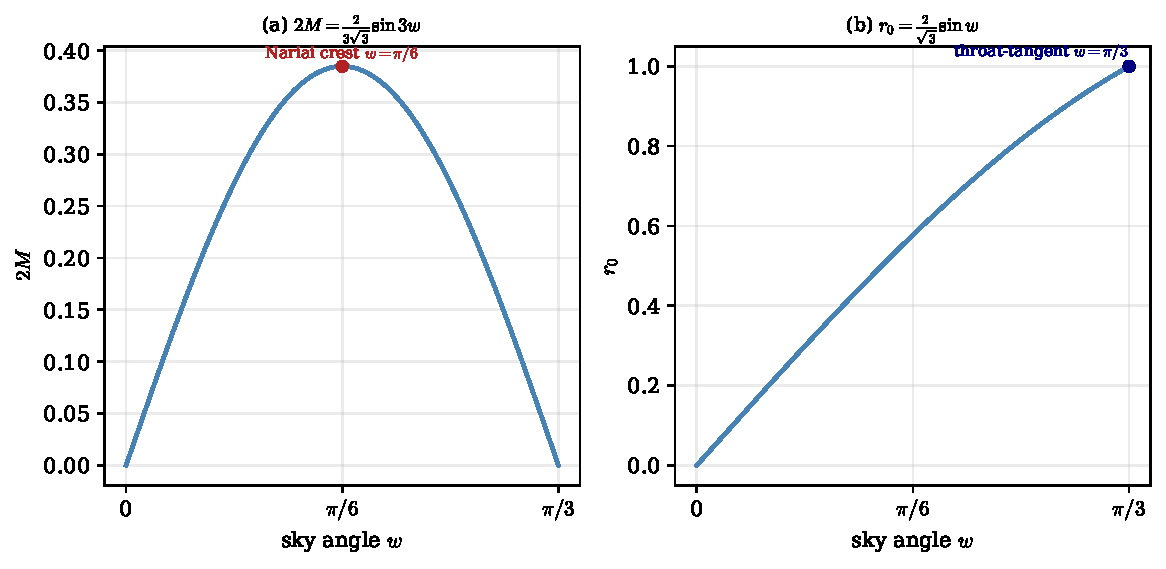
\includegraphics[width=\textwidth]{figs/fig5_triple_angle.pdf}
  \caption{(a) The horizon relation in the sky angle $w$: $2M=\tfrac{2}{3\sqrt3}\sin 3w$,
  a pure triple-angle. A given mass level is met by three sky angles---the three
  horizons; the crest at $w=\pi/6$ is Nariai, where two merge. (b) The slicing
  parameter $r_{0}=\tfrac{2}{\sqrt3}\sin w$, the throat-image radius $2/\sqrt3$
  times the sine of the genuine sky angle: $w\in[0,\pi/3]$ as $r_{0}$ runs
  $[0,1]$, with $w=\pi/3$ the throat-tangent slice.}
  \label{fig:triple}
\end{figure}

The throat circle carries a natural involution of its own: the reflection $g_{1}(x)=\sqrt{1-x^{2}}$ exchanging the two parities of a chart point, which in the throat angle is $u\leftrightarrow\tfrac{\pi}{2}-u$. The cubic involution $\sigma$ is the reflection $w\leftrightarrow\tfrac{\pi}{3}-w$ of the sky angle. Each is a genuine reflection of a genuine geometric angle, and the two are one involution in two coordinates.

\begin{proposition}[Conjugacy]\label{prop:conjugacy}
The chart involution $g_{1}$ and the cubic involution $\sigma$ are conjugate\rcpt{P03_conjugacy},
\begin{equation}\label{eq:chi}
  \chi\circ g_{1}=\sigma\circ\chi,
  \qquad
  \chi(x)=\frac{2}{\sqrt3}\,\sin\!\Bigl(\tfrac{2}{3}\arcsin x\Bigr),
\end{equation}
and the identity holds in closed form.
\end{proposition}

\begin{proof}
Write $x=\sin a$ with $a\in[0,\pi/2]$. Then $g_{1}(x)=\cos a=\sin(\tfrac\pi2-a)$, so
\[
  \chi\bigl(g_{1}(x)\bigr)=\frac{2}{\sqrt3}\sin\!\Bigl(\tfrac23\arcsin\sin(\tfrac\pi2-a)\Bigr)
  =\frac{2}{\sqrt3}\sin\!\Bigl(\tfrac\pi3-\tfrac{2a}{3}\Bigr),
\]
using $\arcsin\sin(\tfrac\pi2-a)=\tfrac\pi2-a$ for $\tfrac\pi2-a\in[0,\tfrac\pi2]$. For the other side, $\chi(x)=\tfrac{2}{\sqrt3}\sin(\tfrac{2a}{3})$, and $\sigma(\xi)=\tfrac12\bigl(-\xi+\sqrt{4-3\xi^{2}}\bigr)$ with $\xi=\chi(x)$ gives, since $4-3\xi^{2}=4\cos^{2}(\tfrac{2a}{3})$ and $\cos(\tfrac{2a}{3})\ge0$ on the range,
\[
  \sigma\bigl(\chi(x)\bigr)=\cos\tfrac{2a}{3}-\tfrac{1}{\sqrt3}\sin\tfrac{2a}{3}
  =\frac{2}{\sqrt3}\sin\!\Bigl(\tfrac\pi3-\tfrac{2a}{3}\Bigr),
\]
the last step by $\tfrac{2}{\sqrt3}\sin(\tfrac\pi3-\vartheta)=\cos\vartheta-\tfrac{1}{\sqrt3}\sin\vartheta$. Both sides equal $\tfrac{2}{\sqrt3}\sin(\tfrac\pi3-\tfrac{2a}{3})$, so $\chi\circ g_{1}=\sigma\circ\chi$ identically.
\end{proof}

The conjugacy is an exact trigonometric identity, not a numerical coincidence: the collapse $4-3\chi^{2}=4\cos^{2}(\tfrac{2a}{3})$ that makes it closed is itself a consequence of the forced slicing scale $2/\sqrt3$. The construction carries a single involution presented two ways---the throat-circle reflection $g_{1}$ and the cubic root-exchange $\sigma$---and $\chi$ is the exact map between them, the natural entry point for the group-theoretic treatment of the companion groupoid paper~\cite{JanzenGroupoid}.

\subsection{The two readings at the throat}\label{sec:two-readings}

Now swing the plane down toward $w=0$. The black-hole horizon shrinks until it merges into $r=0$ at the back; the cosmological horizon swings to the polar-opposite point and becomes the horizon, with $0<r<2M$ wrapping the half-equator and the exterior opening out beyond it. The slicing mass has gone to zero---the black hole has shrunk away---and the cut is now one curve: the equator taken diametrically, which is exactly the companion paper's Schwarzschild curve, the meridian-hyperbola\,$\to$\,equatorial-circle\,$\to$\,meridian-hyperbola of the maximal analytic extension, $r=M(1+\cos z)$ continued through both critical points.

This single $w=0$ curve carries two readings, and the map between them is the backward-radial vantage-swap---this is the de Sitter\,$\leftrightarrow$\,Schwarzschild correspondence, exact, at fixed $\alpha$, and it is neither a limit nor a mass relabelled to zero. Read from the pivot's perspective---the natural reading as the hinge settles to $w=0$, the curve seen from the swing-pivot looking down---it is Schwarzschild: the $2M/r$ term carried perspectivally (the companion paper's reading), the horizon and $r=0$ the two metric singularities of one genus, the curvature at $r=0$ belonging to the perspectival metric over $r$ and not to the underlying manifold. Rotate the vantage through $180^{\circ}$---look from the uphill side, the worldline staring straight up the $r=0$ axis---and the same curve is de Sitter: $f=1-r^{2}/\alpha^{2}$, the cosmological geometry, $r=0$ now the axis rather than a mass-laden centre. One curve, one fixed $\alpha$, two vantages the involution swaps. The underlying invariant geometry is de Sitter; the Schwarzschild mass is the perspectival reading's, carried by the vantage, not a second invariant. This vantage-swap is the mass-reflection $R$, the backward-radial reflection through the $r=0$ branch point; the groupoid paper~\cite{JanzenGroupoid} identifies it as the $A_{2}$ diagram automorphism---the outer $\mathbb{Z}_{2}$ of the solution space's discrete symmetry $\mathrm{Aut}(A_{2})=D_{6}$---with the de~Sitter geometry $1-r^{2}/\alpha^{2}$ and the Schwarzschild mass $-2M/r$ its even and odd parts under the reflection.

We state plainly two routes the construction does \emph{not} take, because each reaches this same throat in a way that breaks the construction. First, Schwarzschild is \emph{not} the $\alpha\to\infty$ limit: $\alpha$ is the fixed invariant the whole construction lives inside, and sending it to infinity dismantles the throat, the circle, and the family in one stroke; the correspondence is reached by swinging the hinge to $w=0$ at fixed $\alpha$ and reading the curve from the pivot, not by deforming the geometry. Second, $r_{0}=0$ is \emph{not} a ``massless Schwarzschild.'' A massless Schwarzschild is a contradiction in terms: Schwarzschild is the geometry with a mass and the cosmological term off, and $M=0$ with the cosmological term on is de Sitter, by definition. Proposition~\ref{prop:r0zero} is right that $r_{0}=0$ carries two readings of one slicing---that is precisely the involution---but the Schwarzschild side is not a massless limit. The slicing mass is zero there because the underlying geometry is de Sitter; the Schwarzschild reading is the pivot-vantage of that same curve, its mass perspectival, $\alpha$ untouched.

Past the Nariai crest the same curve continues overcritically, by the same analytic continuation that joins the seam: $\sin\theta\to\cosh\psi$, equivalently $\theta\to\pi/2+i\psi$ on the horizon angle, $3w=\pi/2+i\beta$. This is not a separate relation and not a redefinition of $w$; its geometry is Section~\ref{sec:seam}.

\subsection{Adding charge: mass is $R$-odd, charge $R$-even}\label{sec:charge}

Reading the eigenspace split of Section~\ref{sec:two-readings} on the charged cut settles, at the geometric level, where charge sits\rcpt{P03_charge_parity} in the construction's one discrete symmetry. The Reissner--Nordstr\"om--de~Sitter slicing function is
\begin{equation}\label{eq:RNdS}
  f(r)=1-\frac{2M}{r}+\frac{Q^{2}}{r^{2}}-\frac{r^{2}}{\alpha^{2}},
\end{equation}
the charge entering, like the mass, on the matter side---a bend of the cut, $m(r)=M-Q^{2}/2r$, sourced by the Maxwell field $A_r=-(Q/r)\,dt$ and not a substrate datum~\cite{JanzenRange}. Under the mass-reflection $R$ ($2M\mapsto-2M$, flipping the geometry to the conjugate branch; Section~\ref{sec:ellipse}) it splits as
\begin{equation}\label{eq:RNsplit}
  f=\underbrace{\Bigl(1-\frac{r^{2}}{\alpha^{2}}+\frac{Q^{2}}{r^{2}}\Bigr)}_{R\text{-even}}\;+\;\underbrace{\Bigl(-\frac{2M}{r}\Bigr)}_{R\text{-odd}},
\end{equation}
so the charge term joins the de~Sitter geometry on the \emph{even} side while the mass remains the odd part the swap reverses. This is a sharp statement about charge, not a formal one. The reading-swap is precisely what exposes the Schwarzschild mass as \emph{perspectival}---the $R$-odd content the vantage carries, a turning point and not a coefficient (Section~\ref{sec:mass})---and it leaves the charge fixed: $Q^{2}/r^{2}$ is reading-swap-neutral, the swap that reverses the mass touching it not at all. Charge is therefore the $R$-\emph{even} matter datum and mass the $R$-\emph{odd} one---both bends of the cut, but of opposite parity under the discrete symmetry the slicing owns, the charge sharing the parity of the \emph{invariant} geometry while the mass shares that of the perspectival vantage. That the mass parameter itself is the odd one, $2M=\alpha\bigl((r_{0}/\alpha)-(r_{0}/\alpha)^{3}\bigr)$ flipping under $r_{0}\mapsto-r_{0}$ (Section~\ref{sec:mass}), is the sky-angle face of the same fact; the charge, an independent parameter the reticle offset does not carry, is untouched by the swap.

Charge conjugation is then geometrically transparent. The slicing function depends on the charge only through $Q^{2}$, so $Q\mapsto-Q$ leaves $f$---and with it the whole slicing curve and every one of its turning points---\emph{identical}: the two signs of charge trace the one curve, the sign living entirely in the Maxwell potential $A$ (linear in $Q$), off the curve. Charge conjugation is thus present on the slicing geometry only as this even $Q\mapsto-Q$ degeneracy---the geometric face of its being field-level---while the full charge conjugation $C$ is antilinear, no geometric reflection at all, and closes from the matter field. And because it is a symmetry of the charge and not of the mass roots the $A_{2}$ system realises---$Q$ absent from the horizon cubic, so $Q\mapsto-Q$ fixes every root---it adjoins an \emph{independent} $\mathbb{Z}_{2}$ to the solution space's $\mathrm{Aut}(A_{2})=D_{6}$ rather than sitting within it: the outer $\mathbb{Z}_{2}$ of $D_{6}$ is the mass-reflection $R$, not charge conjugation. This is the geometric ledger of the boundary paper's second boundary~\cite{JanzenBoundary}. The boundary paper carries it one step further: composed with the antilinear reality involution $\tilde\tau\mapsto\bar{\tilde\tau}$ of the vacuum cosmogenetic bead, the mass-reflection $R$ supplies charge conjugation's geometric \emph{kinematic} (Feynman--St\"uckelberg) face, so that $C$ factorises with only the charge sign closing from the field---and the eigenspace split above is the linear ($R$) root of that positive closure~\cite{JanzenBoundary,JanzenMatter}.

The scope is exact, and worth marking as elsewhere in the construction. The parity result holds on $f$ and its turning-point structure without remainder: the charged horizon relation $-r^{4}/\alpha^{2}+r^{2}-2Mr+Q^{2}=0$ carries $Q$ only as $+Q^{2}$, so the charge shifts the turning points $R$-evenly and $Q\mapsto-Q$ fixes each. What the charge does \emph{not} leave intact is the $r=0$ lap on which the vacuum slicing closes (Section~\ref{sec:lap}): with $Q\neq0$ the term $Q^{2}/r^{2}$ dominates as $r\to0$, so $f\to+\infty$ rather than $-\infty$, an inner (Cauchy) turning point appears, and $r=0$ becomes a timelike Reissner--Nordstr\"om singularity rather than the branch point through which the signed radius passes onto the conjugate branch. The charged closed loop is therefore a genuine extension---the electromagnetic case this paper's closing section names and does not build---whereas the discrete-symmetry reading of charge, mass $R$-odd and charge $R$-even with $C$ its field-level closure, is established here at the level of the slicing function, where it is exact.

\section{The angular tour: the family's discrete skeleton and the hinge geometry}\label{sec:tour}

Read across the full swing $w\in[0,2\pi)$, the family visits three geometries under twelve designations, one every $30^{\circ}$. With $2M=\tfrac{2}{3\sqrt3}\sin 3w$ and $r_{0}=\tfrac{2}{\sqrt3}\sin w$, the mass vanishes ($2M=0$, de~Sitter) at $w=0,60,120,180,240,300^{\circ}$, and reaches its Nariai extremes $2M=\pm\tfrac{2}{3\sqrt3}$ (the double roots, $\kappa=0$) at the intervening $w=30,90,\dots,330^{\circ}$; between the marks the cut is undercritical, three distinct real horizons. Because $|2M|\le\tfrac{2}{3\sqrt3}$ on the real dial, the swing never leaves the undercritical interior except to touch its Nariai boundary. \emph{Read as rangefinding, the $30^{\circ}$ is not a coincidence of the trigonometry but the hole's own angular size}: the hinge stands at $2\alpha$ and the throat has radius $\alpha$, so the hole subtends $\arcsin(\alpha/2\alpha)=30^{\circ}$ there. A sightline within $30^{\circ}$ of the axis cuts the throat, one at $30^{\circ}$ grazes it, and one beyond misses. \emph{So the dial's endpoint is the grazing sightline, and Nariai is the hole's limb}---the extreme of the swing and the edge of the aperture being one angle read two ways\ldg{figure_theorem}. \emph{And the trichotomy the dial runs through is the conic trichotomy of that same sightline.} Take the slicing plane at transverse distance $d$ from the axis and cut the substrate $-x_{0}^{2}+\lvert X\rvert^{2}=\alpha^{2}$ with it. For $d>\alpha$ the section is a two-sheeted hyperbola whose vertex stands at height $\sqrt{d^{2}-\alpha^{2}}$---and at the dial's end, $d=2\alpha$, that vertex is $\sqrt3\,\alpha$, \emph{which is the hinge}: the hinge is the vertex of the extreme sightline. For $d<\alpha$ the plane cuts the throat and the corresponding point is the secant's midpoint instead. \emph{And at $d=\alpha$ the section degenerates into two straight lines, and those lines are null}---$x_{0}=\pm y$, so $\dd s^{2}=-\dd x_{0}^{2}+\dd y^{2}=0$---so the cut at Nariai \emph{is} the substrate's two rulings. Miss, touch and cut are therefore two-sheeted hyperbola, two null rulings, and two horizons: \emph{one locus, one turning plane, and the same three outcomes the horizon cubic gives}\ldg{figure_theorem}. What follows: the strict overcritical regime is reached by no real swing, but only by the imaginary continuation past a crest (Section~\ref{sec:seam}).

The six Nariai marks are the $A_{2}$ hexad. The three at $2M=+\tfrac{2}{3\sqrt3}$ ($w=30,150,270^{\circ}$) carry the root triple $(-2,1,1)/\sqrt3$, whose directions are those of a fundamental $\mathbf 3$'s weights taken at root normalisation---the triple has $|v|^{2}=2$, the root length, against the weights' own $2/3$, the two hexagons differing by a rotation of $30^{\circ}$ and a factor of $\sqrt3$\ldg{representation_theory}; the three at $2M=-\tfrac{2}{3\sqrt3}$ ($w=90,210,330^{\circ}$) carry its negation $(2,-1,-1)/\sqrt3$, the antifundamental $\bar{\mathbf 3}$; and the parity $R:2M\mapsto-2M$ (equivalently $r_{0}\mapsto-r_{0}$) exchanges them.\footnote{Corpus convention: $R$ denotes this orientation/mass-reflection parity---the $A_{2}$ diagram automorphism, the orientation-reversing element $\mathrm{O}(5,1)\setminus\mathrm{SO}_{0}(5,1)$, realised on a cut spinor as $\gamma^{5}$ in the matter-sector papers~\cite{JanzenGroupoid,JanzenBoundary}. It is \emph{not} the areal spatial parity $r\mapsto-r$ (Clifford generator $\gamma^{1}\gamma^{2}\gamma^{3}$, which anticommutes with $\gamma^{5}$), for which the corpus reserves ``$P$''; that spatial parity does not appear in this paper. The time reflection $X_{0}\mapsto-X_{0}$ is $T$ throughout.} The full automorphism group $\mathrm{Aut}(A_{2})=S_{3}\times\mathbb{Z}_{2}\cong D_{6}$ acts on the dial as the symmetry of a regular hexagon---the rotation $w\mapsto w+60^{\circ}$ (order six, $2M\mapsto-2M$) and the reflection $w\mapsto-w$---with the six Nariai its vertices and fundamental domain $[0,30^{\circ}]$; its group-theoretic form is obtained in the groupoid paper~\cite{JanzenGroupoid}. \emph{Read as $A_{2}$'s own chamber structure the three counts on the dial are one fact rather than three}: the discriminant vanishes exactly at the six marks, so those are the \emph{wall-crossings}; the six arcs between them are the six Weyl chambers, $|W(A_{2})|=|S_{3}|=6$; and the twelve designations are $|\mathrm{Aut}(A_{2})|=12$, two to an arc. \emph{The sign of $2M$ is then the chamber's own $\mathbb{Z}_{2}$ label}, which is why $R$ \emph{is} the diagram automorphism exchanging $\mathbf3$ and $\bar{\mathbf3}$ rather than merely analogous to one.

\subsection{The hinge geometry}\label{sec:hinge-geometry}

The swing-pivot of Section~\ref{sec:slicing}---the hinge---sits at transverse distance $2\alpha$ from the hole's axis, the vantage from which the throat subtends exactly $60^{\circ}$ (angular radius $\arcsin\tfrac12=30^{\circ}$). The three hinges of the three $120^{\circ}$-separated vantages form an equilateral triangle of circumradius $2\alpha$ whose incircle, of radius $\alpha$, is the throat itself: the hole is the incircle of the hinge triangle (Figure~\ref{fig:keplerian}). Its three sides are not imposed but \emph{found}---each is a null generator of the doubly-ruled substrate (Section~\ref{sec:slicing}), tangent to the throat at its midpoint.

\paragraph{The distance $2\alpha$ is not chosen.} Stated as above the hinge's placement reads as a stipulation, and it is not one: it is the only distance the hole itself names, and every other number in the figure follows from it.\rcpt{alpha_alone} Ask where a hinge \emph{could} go. The construction has one input, the hole---a circle of radius $\alpha$ about the axis---and $\alpha$ is not a number but the gauge. The one circle the hole determines without further choice is the circle on its own edge through its own centre: centre $(\alpha,0)$, radius $\alpha$, the hole translated onto its edge. That circle \emph{ends} at $2\alpha$, and the hinge is its far end. So $2\alpha$ is an output. The one input is the whole of it: what this paper reads off that circle---the hinge's placement, the $60^{\circ}$ subtense, the incircle and nine-point relations, the tangency that returns Nariai, and the walls the signed radius sets on its rim---the geometric-core paper collects with the circle's other faces (its radius \emph{is} the curvature; its tangents \emph{are} the null rulings; the power of a point with respect to it is that point's height) as the seventh face of the substrate's maximal symmetry~\cite{JanzenGeometricCore}.

\begin{proposition}[The hinge's placement, and what follows from it]\label{prop:twoalpha}
Let the hinge sit at transverse distance $R$ from the axis. The following are equivalent:
\begin{enumerate}\itemsep0pt
\item $R=2\alpha$;
\item the throat subtends $60^{\circ}$ at the hinge, i.e.\ $\arcsin(\alpha/R)=30^{\circ}$;
\item the hinge triangle's sides are tangent to the throat \emph{at their midpoints}---an equilateral triangle's inradius is half its circumradius, so midpoint-tangency holds iff $R=2\alpha$;
\item the nine-point circle of the hinge triangle \emph{is} the throat\rcpt{euclid7_nine_point}---by Euler's theorem the nine-point radius is $R/2$ and its centre is the equilateral's own centre;
\item the tangent length from the hinge to the throat equals the hinge's height in the embedding, both $\sqrt3\,\alpha$;
\item writing $s^{2}$ for the squared separation of two opposite-horn ends of a $120^{\circ}$-separated triple of lines at transverse radius $R$, one has $s^{2}=4\alpha^{2}-R^{2}$, so $R=2\alpha$ is the unique transverse radius at which those pairs are \emph{null}\rcpt{P03_the_sixth_equivalence}.
\end{enumerate}
\end{proposition}

\noindent Each equivalence is a line, and the point is not any one of them but their number: the incircle relation this section already states, the $60^{\circ}$ it already computes, and the height $\sqrt3\,\alpha$ that Figure~\ref{fig:keplerian} already carries are not several facts about the hinge but one fact wearing several faces. Item~(iv) is worth marking because it reaches the placement by a route mentioning neither tangency nor the subtended angle nor the substrate---Euler's $R/2$, and nothing else. Item~(vi) differs from the other five in \emph{kind} rather than in content, and is worth marking for that reason: the first five are statements about a Euclidean figure, while the sixth reads the same placement in the substrate's own causal language---$2\alpha$ is where the opposite-horn pairs go null---so the count above is not five Euclidean faces but five and one causal. Item~(v) is the substrate's own in a different sense: the tangent runs $\sqrt3\,\alpha$ across while the hinge stands $\sqrt3\,\alpha$ high, so the sightline is null and $\tan 60^{\circ}=\sqrt3$ is that one length against the throat radius (the tangent's null character is the geometric-core paper's, \cite{JanzenGeometricCore}). The equivalences are verified in the programme's figure-theorem ledger and its receipts (\texttt{FIGURE\_THEOREM\_LEDGER.md}; \texttt{alpha\_alone.py}, \texttt{one\_thirty.py}, \texttt{euclid7\_nine\_point.py}), where the wider catalogue of classical theorems read on this figure is collected.

The placement then \emph{forces the Nariai configuration}, by the triple angle and nothing else.\rcpt{one_thirty} The subtended half-angle $30^{\circ}$ is the sky angle $w$ of Section~\ref{sec:projection}, so $\sin w=\tfrac12$, and the horizon relation $2M=\tfrac{2}{3\sqrt3}\sin 3w$ of Section~\ref{sec:throat-angle} gives
\begin{equation}\label{eq:tripleathinge}
\sin 3w \;=\; 3\sin w-4\sin^{3}w \;=\; 3(\tfrac12)-4(\tfrac12)^{3} \;=\; 1,
\end{equation}
its maximum. The tangent from the hinge is therefore the Nariai cut---not because two angles of $30^{\circ}$ coincide, but because the identity peaks there of its own accord once the hole has placed the hinge. The chain from the single input runs
\[
\text{the hole } \alpha \;\longrightarrow\; \text{hinge at } 2\alpha \;\longrightarrow\; \sin w=\tfrac12 \;\longrightarrow\; \sin 3w=1 \;\longrightarrow\; 3w=90^{\circ} \;\longrightarrow\; w=\tfrac{360^{\circ}}{3\times4}=30^{\circ},
\]
whose last step is the $30^{\circ}$ spacing of the twelve designations of Section~\ref{sec:tour}: a sine peaks a quarter-turn from its zero, so the $4$ is the sine's own and the $3$ is the triple angle's, and $12=3\times4$ has both factors forced by one route.

\begin{figure}[htbp]
\centering

\includegraphics[width=0.54\textwidth]{figures/CR_keplerian_hinge_structure.png}
\caption{The Keplerian hinge structure. The hole (throat circle, radius $\alpha$) is the incircle of the equilateral of three hinges (circumradius $2\alpha$, polar angles $0/120/240^{\circ}$); the three sides are the Nariai double null rulings, tangent to the throat at their midpoints. The dual rulings cross above and below the equatorial plane at $X_{0}=\pm\sqrt3\,\alpha$ on the hyperboloid $-X_{0}^{2}+X_{1}^{2}+X_{2}^{2}=\alpha^{2}$. Six hinge vertices (three up, three down); one swings the door in the vacuum construction, while the matter sector places a plane on each of the three~\cite{JanzenMatter}; the hole subtends $60^{\circ}$ from each hinge.}
\label{fig:keplerian}
\end{figure}

A word on what is being counted, since the construction's habitual phrase ``the six hinges'' names the piercings after the thing that makes them. \emph{The hinge is the line the door swings on} (Section~\ref{sec:slicing}): a line parallel to the hole's axis at transverse radius $2\alpha$, which does not translate. There are \emph{three}. Such a line is not contained in the substrate---its direction is timelike, so it is none of the substrate's null rulings---and it therefore \emph{pierces} the hyperboloid rather than lying in it, once on each horn, at $X_{0}=\pm\sqrt3\,\alpha$. The six points below are accordingly \emph{three hinges with two ends apiece}, $3\times2$ and not $6$ (Figure~\ref{fig:U3}a), and the distinction is load-bearing twice over: it is why the construction has exactly \emph{one} dial---the ambient planes containing a fixed \emph{line} form a pencil, which is one-parameter, where a pivot that were a \emph{point} would leave a two-parameter family---and it is what Remark~\ref{rem:hingetriple} turns on.

Followed in the embedding rather than the equatorial projection, each such null ruling runs from a hinge's end on one horn, tangent to the equatorial throat, to the end of a \emph{different} hinge on the \emph{opposite} horn: the ruling through a throat point places the two ends it joins at transverse radius $2\alpha$ and heights $X_{0}=\pm\sqrt3\,\alpha$ on the hyperboloid $-X_{0}^{2}+X_{1}^{2}+X_{2}^{2}=\alpha^{2}$. The six hinge-ends---three upper ($X_{0}=+\sqrt3\,\alpha$), three lower ($X_{0}=-\sqrt3\,\alpha$)---close into a single skew hexagon of null rulings,
\[
  U_{0}\to D_{120}\to U_{240}\to D_{0}\to U_{120}\to D_{240}\to U_{0},
\]
each edge tangent to the throat at its midpoint (Figure~\ref{fig:skewhex}). The upper and lower triangles are exchanged by the time reflection $X_{0}\mapsto-X_{0}$, which swaps the two null generators; and since each of the three hinge-lines designates one horizon root (below), the upper triangle reads as the three roots, the fundamental $\mathbf 3$. Whether the lower triangle is properly the antifundamental $\bar{\mathbf 3}$, and whether this six-fold is the \emph{same} hexad as the $A_{2}$ hexad of the six Nariai---which the mass-reflection parity $R:r_{0}\mapsto-r_{0}$ exchanges as $\mathbf 3\oplus\bar{\mathbf 3}$---is a genuine \emph{resonance} and not an identity. $R$ (the transverse-offset reflection, the $A_{2}$ diagram automorphism) reflects a \emph{spacelike} leg, while the time reflection $T:X_{0}\mapsto-X_{0}$ reflects the \emph{timelike} ambient one; on the six vertices $T$ flips the horn ($X_{0}=+\sqrt3\,\alpha\mapsto-\sqrt3\,\alpha$) while $R$ preserves it, so $R\neq T$ pointwise---$R$ fixes $U_{0}$ where $T$ sends it to $D_{0}$ (a spacelike and a timelike reflection cannot coincide). The upper triangle is the shared fundamental $\mathbf 3$; its two completions to the hexad---the lower triangle by $T$, and the proper $\bar{\mathbf 3}$ by $R$---are therefore distinct, so the lower triangle is the $T$-image, not the proper $\bar{\mathbf 3}$. The two hexads share the fundamental triple but complete by distinct reflections, related by their product $R\circ T$ (itself a hexad symmetry): a resonance, not an identity.

The hexagon's own incidence structure is worth reading off, since it says why a hexagon is the only closed
figure these rulings can make. Under the Klein correspondence a line of $\mathbb{P}^{3}$ becomes a point of a
quadric and two lines meet exactly when their points are conjugate; carrying the six edges over, each meets
three of the others---its two neighbours \emph{and its opposite}---and the six split into two triples within
which no two meet\rcpt{D2_hexagon_klein}. That is the signature of the two ruling families: same family skew,
opposite families meeting. So the alternation is forced, and with it the length: a closed circuit alternating
between the families must have even length, and six is the least that visits all six hinge-ends. The three
opposite-edge crossings then land at $X_{0}=0$, on the throat itself, at the three points where the projected
hinge triangle touches it---the midpoints of Proposition~\ref{prop:twoalpha}(iii), which the geometric-core
paper independently identifies as the vertices of the figure's projective dual~\cite{JanzenGeometricCore}. One
triple, and the faces it carries are worth listing in full rather than in part, since each was reached by a
different route and no one of them mentions the others: the tangency points of the projection; the
\emph{midpoints} of the hinge triangle's sides (Proposition~\ref{prop:twoalpha}(iii)); the vertices of the dual
figure~\cite{JanzenGeometricCore}; the crossings of the skew hexagon's opposite edges; the points at which the
substrate's null generators through the punctures graze the throat; the loci at which the matter sector places
its throat walls~\cite{JanzenMatter}; and the $r=0$ branch points through which the signed radius laps
(\S\ref{sec:lap}).\rcpt{P03_locus_sweep} \emph{Seven descriptions and one place.} The last two are the ones that
carry weight elsewhere in the programme, and neither had been drawn against the first five.

\begin{remark}[The causal trichotomy of the hinge-ends, and a $2{+}1$ whose assignment is relative]\label{rem:hingetriple}
The paragraph above reads the hexagon's incidence on its \emph{edges}. Read instead on its \emph{vertices}---the six hinge-ends---the same figure classifies completely, and the classification is causal. Two points of the substrate are null-separated exactly when $X\cdot Y=\alpha^{2}$; for two ends at stations $a,b$ on horns $\varepsilon,\varepsilon'=\pm1$,
\[
  X\cdot Y=\alpha^{2}\bigl(-3\varepsilon\varepsilon'+4\cos(\theta_{a}-\theta_{b})\bigr),
\]
and the fifteen pairs fall into exactly three classes, each of which encodes exactly one shared label\rcpt{P03_hexagon_null_triple}:
\[
  \text{timelike}\iff\text{same hinge}\ (3),\qquad
  \text{spacelike}\iff\text{same horn}\ (6),\qquad
  \text{null}\iff\text{neither}\ (6).
\]
So every hinge-end is null-joined to exactly two others, both on the opposite horn and both belonging to \emph{other} hinges---six vertices of degree two, bipartite between the horns, which is why the closed figure is a hexagon and why it alternates. The alternation was inferred above from the two ruling families; here it is a property of the vertices, and the two readings agree. The two pairs the null relation omits are not omissions of the same kind: two ends of one hinge \emph{cannot} be null-separated, the hinge being timelike, so the pair a null binding appears to exclude is the hinge itself seen at its two piercings; and two ends on one horn are spacelike. The substrate's causal structure is thus the whole bookkeeping of the hinge and horn labels, and nothing further is needed to read them.

There is a second count on the same figure, and it is the one that sees the tangencies. Through each puncture run \emph{both} of the substrate's rulings, so the configuration carries $6\times2=12$ null \emph{legs}, each running from a puncture to the equatorial point at which it grazes the throat; two legs meeting at a graze point make one chord, and the twelve legs graze at only \emph{three} points---$60^{\circ}$, $180^{\circ}$, $300^{\circ}$, each lying directly between two hinges, four legs apiece---so that $6\times2=3\times4=12$ and the count closes both ways (Figure~\ref{fig:U3}).\rcpt{P03_twelve_null_legs} That both rulings through a puncture run on through a \emph{further} puncture is not automatic: the substrate carries a two-parameter family of rulings, and this is a property of the $2\alpha$ placement, which Proposition~\ref{prop:twoalpha} obtains as an output rather than assuming. The three graze points are the side midpoints of Proposition~\ref{prop:twoalpha}(iii), which the geometric-core paper independently reaches as the vertices of the figure's projective dual~\cite{JanzenGeometricCore}. They are also, and this is not a further coincidence but the same three points a third time, the loci at which the matter sector places its throat walls: that construction fixes them as the signed radius's $r=0$ point on the throat circle---the back of the hole, taken relative to the hinge whose plane swings---and so obtains a $\mathbb{Z}_3$ orbit each of whose members is antipodal to a hinge~\cite{JanzenMatter}. The two derivations share nothing: one runs on the signed radius, the other on null tangency.\rcpt{P03_wall_is_the_graze_point} Read together they say that a hinge's wall is the point at which the \emph{other two} hinges' null tangents meet the throat, so that the hinge-to-wall assignment is the antipodal map and carries no handedness; and that a hinge's own two legs graze at the other two hinges' walls and never at its own, which is the $1+2$ of this section appearing once more and now on the walls (Figure~\ref{fig:U3}b).

Counted this way the triple comes with a \emph{pair} of graze points, and they are not arbitrarily placed: they sit at exactly $-60^{\circ}$ and $+60^{\circ}$ from the triple's own hinge azimuth---mirror images in that azimuth, being the left and right tangents from the hinge to the throat, with no third option available. Each such tangent is a Nariai cut, by the chain already run above: the subtended half-angle is the sky angle, $\sin w=\tfrac12$, whence $\sin3w=1$ and $r_{0}=\tfrac{2}{\sqrt3}\sin w=\pm1/\sqrt3$. \emph{So a triple's two legs are the Nariai member at positive and at negative gnomonic angle}, and the handedness distinguishing them is graded by $r_{0}\mapsto-r_{0}$---the offset parity $R$, which is the same involution the fermion sector reads as the chirality operator~\cite{JanzenMatter} and under which mass is odd and charge even (Section~\ref{sec:charge}). That three separately established facts meet on one pair of legs is recorded here as structure; what it is worth is not this paper's to say.

Two further consequences. First, the projection to the equatorial plane is \emph{two-to-one}: the six null chords project onto the three sides of the hinge triangle, two apiece---$U_{i}\to D_{j}$ and $U_{j}\to D_{i}$---so each side carries both of the substrate's rulings through it, the two told apart by which horn they run from. The triangle is a shadow in which the two rulings coincide, and Proposition~\ref{prop:twoalpha}(iii)'s midpoint tangency is accordingly a statement about the shadow of a pair. That projection is a regular two-fold covering and its deck transformation is $T$: the six ends cover the three hinge lines two-to-one and the six chords cover the three sides two-to-one, with the horn label distinguishing the sheets, so the order-twelve symmetry $D_{6}=S_{3}\times\mathbb{Z}_{2}$ is the symmetry \emph{of the cover}---$S_{3}$ the triangle's own symmetry below, $\mathbb{Z}_{2}$ the deck group, and the direct product exactly the statement that the deck commutes with the triangle's symmetries. So ``doubly ruled'' below and ``two-sheeted'' above are one fact, and this construction's $\mathbb{Z}_{2}$ carries three descriptions---horn swap, second ruling, deck of the covering---which are here identified.\rcpt{P03_colour_spacelike_isospin_timelike} Second, the causal reach from any end splits the three \emph{hinges} as $\{$one's own, reached timelike$\}$ against $\{$the other two, reached null$\}$: a $2{+}1$ on three objects, carried by a relation of the substrate rather than by a labelling of it, and so distinct in kind from the two the family's algebra supplies---the designation split of Section~\ref{sec:cubic}, graded by $\sigma$, and the sign split, graded by the offset parity $R$. It is a third such split, and the paragraph below decides it: the configuration's symmetry acts transitively on the six ends with a single orbit on each causal class, so the causal $2{+}1$'s assignment is relative and no invariant of the configuration fixes it---whereas $r_{0}$ is the cut's own parameter and no element of that symmetry moves it. A split the symmetry randomises is not a split the symmetry determines. The sign split is excluded on the same ground and on a second one, that it changes across $|r_{0}|=1$ while the causal split is the same $2{+}1$ at every member of the family.

What must be said about that $2{+}1$, because it is easily mistaken for an incompleteness, is that \emph{its assignment is relative and no invariant of the configuration can fix it}. The configuration's symmetry group---the dihedral symmetry of the three stations together with the horn swap $T$, of order twelve---acts transitively on the six ends, and with a single orbit on each of the three causal classes.\rcpt{P03_hexagon_null_triple} Causal character is therefore a \emph{complete} invariant of a pair: there is no finer one to be found, because no orbit remains to distinguish. The $2{+}1$ is a real feature of the figure and is well-posed only once a vantage is chosen, every vantage being equivalent to every other. A construction that singled one reading out absolutely would be asserting a distinction its own symmetry forbids---and the corpus reads its discrete species labels the same way, the mass-reflection $R$ relating $\mathbf3$ and $\bar{\mathbf3}$ without privileging either. Where a distinction between two such complementary readings could come from, if it comes from anywhere, is not this figure: Section~\ref{sec:charge} establishes that the slicing function carries charge only as $Q^{2}$, so $Q\mapsto-Q$ fixes every horizon root and adjoins a $\mathbb{Z}_{2}$ \emph{independent} of $\mathrm{Aut}(A_{2})=D_{6}$ rather than sitting within it. That this is the right shape for such a distinction is noted and not claimed; testing it is not this paper's work.
\end{remark}

\begin{figure}[htbp]
\centering
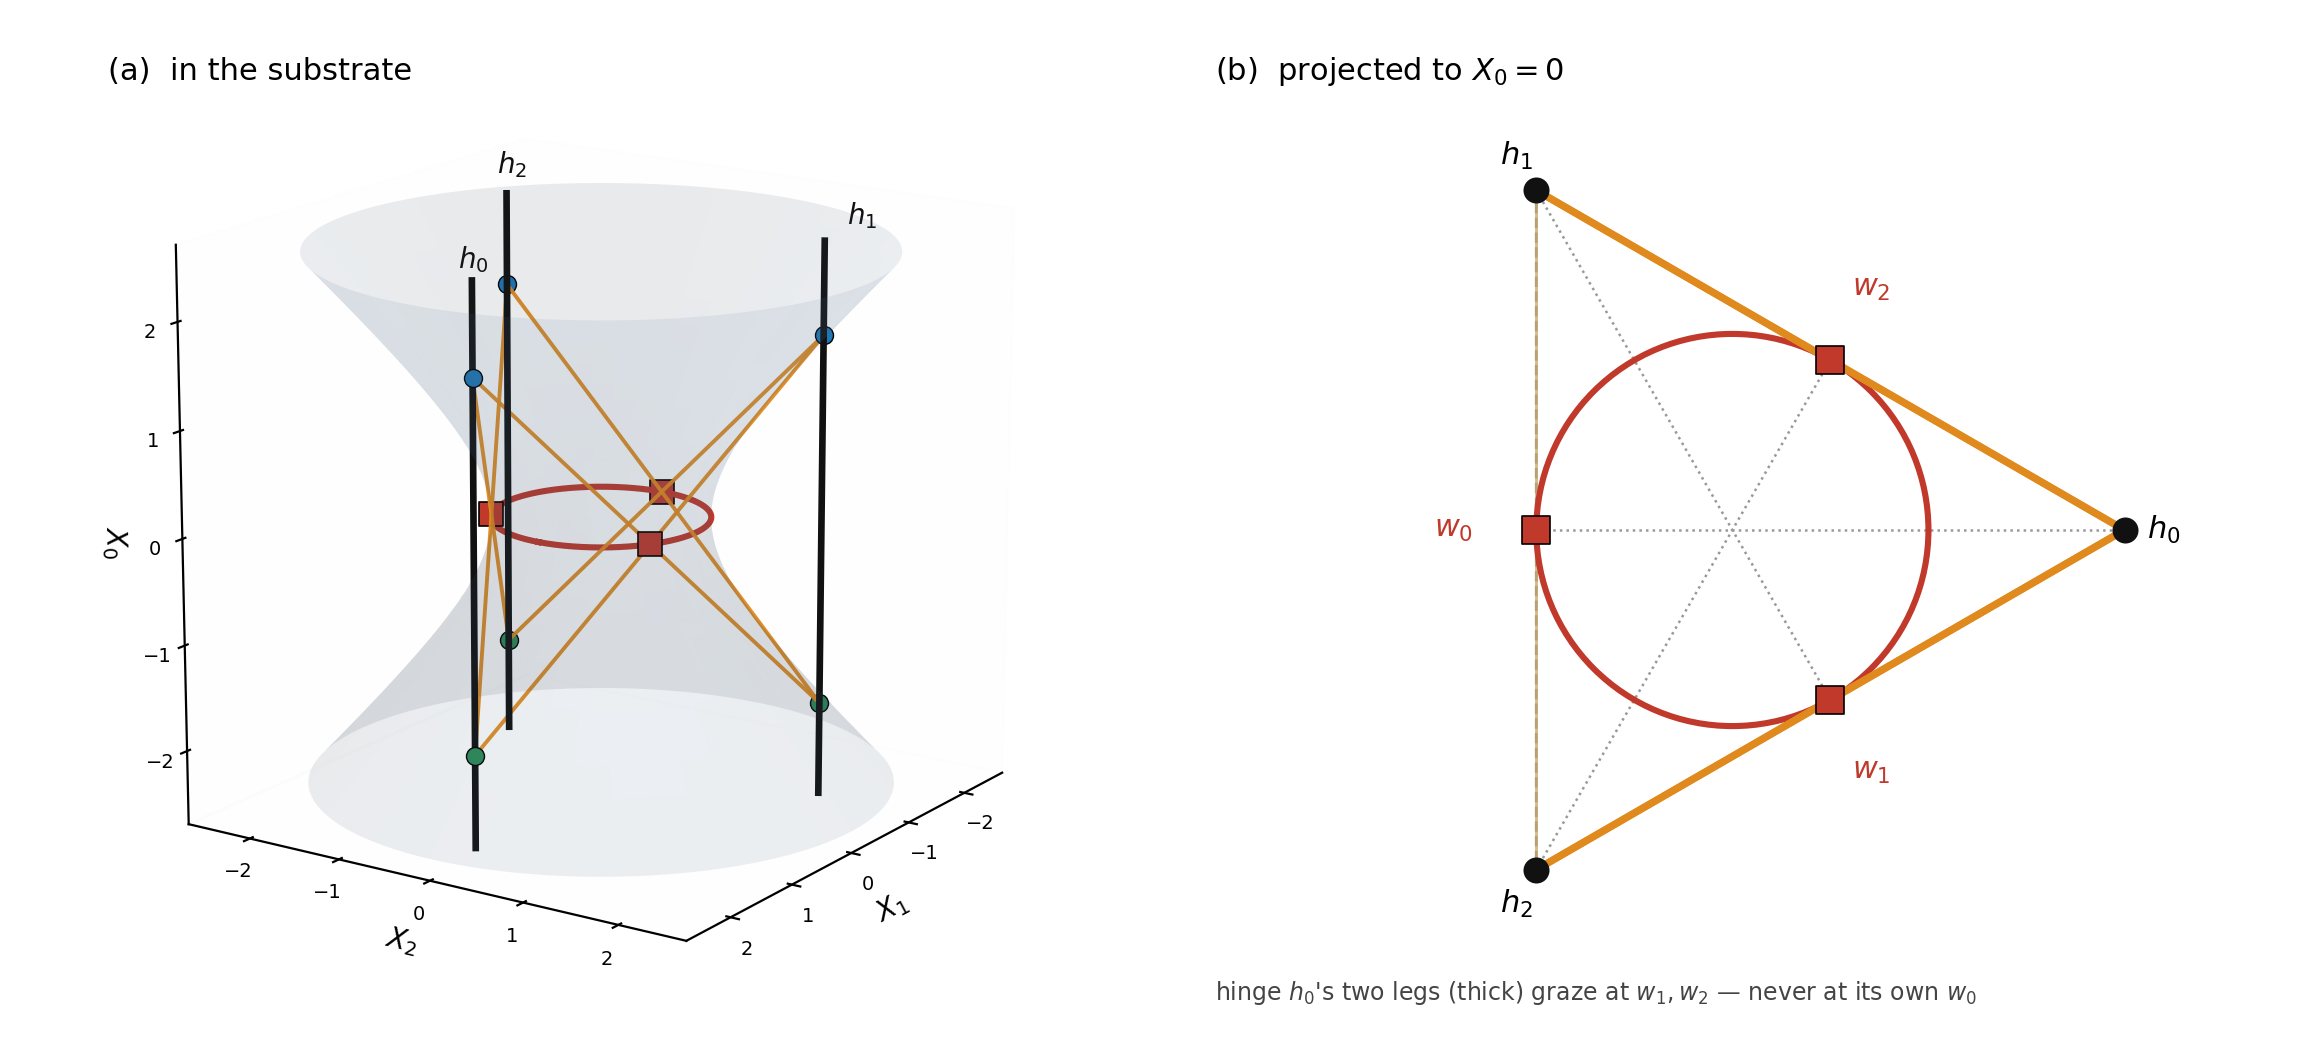
\includegraphics[width=\textwidth]{figures/CR_hinge_substrate_U3.png}
\caption{The hinge structure entire, drawn once.\rcpt{P03_the_U3_figure} \emph{(a)} In the substrate $-X_{0}^{2}+X_{1}^{2}+X_{2}^{2}=\alpha^{2}$: \emph{three} hinges $h_{0},h_{1},h_{2}$ (black), each a \emph{line} parallel to the hole's axis at transverse radius $2\alpha$ and at azimuth $0/120/240^{\circ}$, whose timelike direction is none of the substrate's rulings, so that each \emph{pierces} the hyperboloid once per horn, at $X_{0}=\pm\sqrt3\,\alpha$---six punctures, upper (blue) and lower (green), $3\times2$ and not $6$. Both rulings run through each puncture, giving $6\times2=12$ null legs, which pair into the six chords drawn (orange), each running from a puncture on one horn to a puncture of a \emph{different} hinge on the other, and each tangent to the equatorial throat (red, radius $\alpha$) at its own midpoint. The twelve legs graze at only \emph{three} points (red squares), so that $6\times2=3\times4=12$ and the count closes both ways. \emph{(b)} The same configuration projected orthogonally to $X_{0}=0$, where the projection is two-to-one---the six chords fall onto the three sides of the hinge triangle, two apiece, the pair told apart by which horn it runs from---and the throat is the triangle's incircle (Proposition~\ref{prop:twoalpha}). The three graze points are the side midpoints, and are the loci at which the matter sector places its throat walls~\cite{JanzenMatter}: $w_{k}$ is \emph{antipodal} to $h_{k}$ (dotted), so the hinge-to-wall assignment carries no handedness. Picked out in bold is what that assignment forces---a hinge's own two legs graze at the \emph{other two} hinges' walls and never at its own, this section's $1+2$ appearing once more and now on the walls. The two legs of a given hinge leave it at $\pm60^{\circ}$ from its azimuth, mirror images in it, and each is a Nariai cut at gnomonic angle $r_{0}=\pm1/\sqrt3$, the pair graded by the offset parity $R$.}
\label{fig:U3}
\end{figure}

\begin{figure}[htbp]
\centering
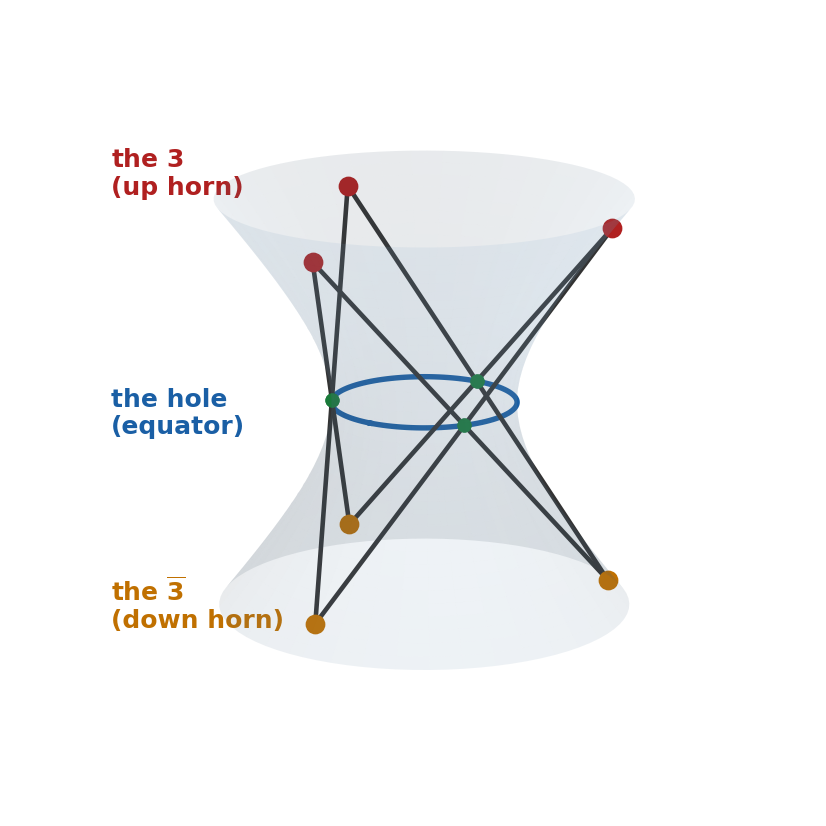
\includegraphics[width=0.54\textwidth]{figures/CR_skew_hexagon_A2.png}
\caption{The $A_{2}$ hexad in the substrate. \emph{Three} hinges---each a line at transverse radius $2\alpha$, piercing the hyperboloid once per horn---give six ends, three upper ($X_{0}=+\sqrt3\,\alpha$, the $\mathbf 3$) and three lower ($X_{0}=-\sqrt3\,\alpha$, the $\bar{\mathbf 3}$), which close into one skew hexagon of null rulings, $U_{0}\to D_{120}\to U_{240}\to D_{0}\to U_{120}\to D_{240}\to U_{0}$, each edge tangent to the equatorial throat at its midpoint. The upper and lower triangles are exchanged by the time reflection $X_{0}\mapsto-X_{0}$, which swaps the two null generators. Whether this six-fold is the same hexad as the $A_{2}$ hexad of the six Nariai (exchanged as $\mathbf 3\oplus\bar{\mathbf 3}$ by the distinct offset parity $R:r_{0}\mapsto-r_{0}$) is a resonance, established here as \emph{not} an identity: $T$ (timelike, horn-flipping) and $R$ (spacelike, horn-preserving) are distinct reflections, so $U\oplus D$ (completed by $T$) and $\mathbf 3\oplus\bar{\mathbf 3}$ (completed by $R$) share the fundamental triple but complete distinctly.}
\label{fig:skewhex}
\end{figure}

These three hinges make the root-exchange involution $\sigma$ (Section~\ref{sec:cubic}) physical. Each hinge designates one of the three horizon roots its swing produces as \emph{its own} black-hole horizon; $\sigma$, which swaps which root is so designated, is the step to a neighbouring hinge---the vantage for which a point one hinge reads as cosmological is read as the black-hole horizon instead. A transposition of roots is a hop to a neighbour, the full three-cycle the tour around all three, and the Weyl group $S_{3}$ that permutes the roots is thus not an abstract relabelling but the relation among the three vantages: reading the one geometry from the next hinge over. This is what the fermion sector reads: a spinor on the slicing structure binds one chiral zero-mode at each hinge's wall, one per vantage---identical in content, since every root returns the same $2M$, and distinguished by which root each takes as its own hole, which is the same distinction as which wall each binds at~\cite{JanzenMatter}. \emph{What that three then indexes is revised in the sector that owns it, and this paper follows the revision}: the matter paper withdraws the reading of these three vantages as the three \emph{generations} and reads them as a \emph{within-state} index instead, the generations' own threeness being carried by the turnaround's deck $\mathbb{Z}_{3}$---a three that paper proves affinely inequivalent to this one---while what the wall structure fixes is the \emph{number}~\cite{JanzenMatter}. And both structures the substrate's discrete residue acts on are relations to the throat circle: the three roots are three special points \emph{on} it---the offset line meets it at two, the third being $r=0$ fixed at the back (\S\ref{sec:hinge-geometry})---while the two null rulings are the lines \emph{tangent} to it, tangency and nullity being one condition here~\cite{JanzenGeometricCore}. Since \emph{on} and \emph{tangent} are independent relations, the residue's two factors act on independent structures, which is why $\mathrm{Aut}(A_{2})$ is a direct product~\cite{JanzenAlgebroid}; and since a tangent is a line of the substrate while a root labels a different cut, they differ in kind, the reading stated on the sector where they become matter~\cite{JanzenMatter}. The mass-reflection parity $R:r_{0}\mapsto-r_{0}$ (the $A_{2}$ diagram automorphism), which carries $\mathbf 3$ to $\bar{\mathbf 3}$, is geometrically a swap of the two null generators---distinct from the time reflection $X_{0}\mapsto-X_{0}$ that exchanges the two horns, though both swap the rulings. The discrete symmetry of Section~\ref{sec:cubic} and the observer-groupoid of Section~\ref{sec:groupoid} are the shadow this hinge relation throws.

That the maximally symmetric substrate carries this discrete $A_{2}$ skeleton---the hexad, the $\mathbf 3\oplus\bar{\mathbf 3}$, and its parity---is a structural fact of the construction. The bridge to matter this poses is built~\cite{JanzenMatter}: a propagating spinor on the slicing structure carries the parity $R=\gamma^5$ as its chirality operator and realises the $\mathbf 3\oplus\bar{\mathbf 3}$ as the fermion sector's content~\cite{JanzenMatter}, so within CR the fundamental $\mathbf 3$ the hinges designate is matter and the antifundamental $\bar{\mathbf 3}=R(\mathbf 3)$ its antimatter, the two the substrate's one $R$-parity relates---at the same weight, forced within CR, the world-correspondence of the identification remaining the data's to judge as it does for the matter it pairs. What the geometry does \emph{not} supply---on either side of that pair equally---is the charge structure, which is field-level~\cite{JanzenBoundary} (its reading-swap parity---charge $R$-even, joining the invariant geometry, $C$ the field-level closure---worked out in Section~\ref{sec:charge}); the parity supplies the discrete matter/antimatter skeleton, not the charge that closes $C$. Whether the continuous $\mathrm{SU}(3)$ whose fundamental and antifundamental share this abstract root system is the physical colour is the residual question: the geometric-isometry route to it is excluded ($\mathfrak{su}(3)\not\subset\mathfrak{so}(5,1)$), but the boundary and geometric-core papers place that $\mathfrak{su}(3)$ on the substrate's conjugate real form---the $S^{5}=\mathrm{SO}(6)/\mathrm{SO}(5)$ the global Wick reaches---so what is left open is whether it is the physical colour, not its geometric home~\cite{JanzenBoundary,JanzenGeometricCore}; the discrete $\mathbf 3\oplus\bar{\mathbf 3}$ matter/antimatter skeleton is not that question and does not wait on it.

\begin{figure}[htbp]
\centering
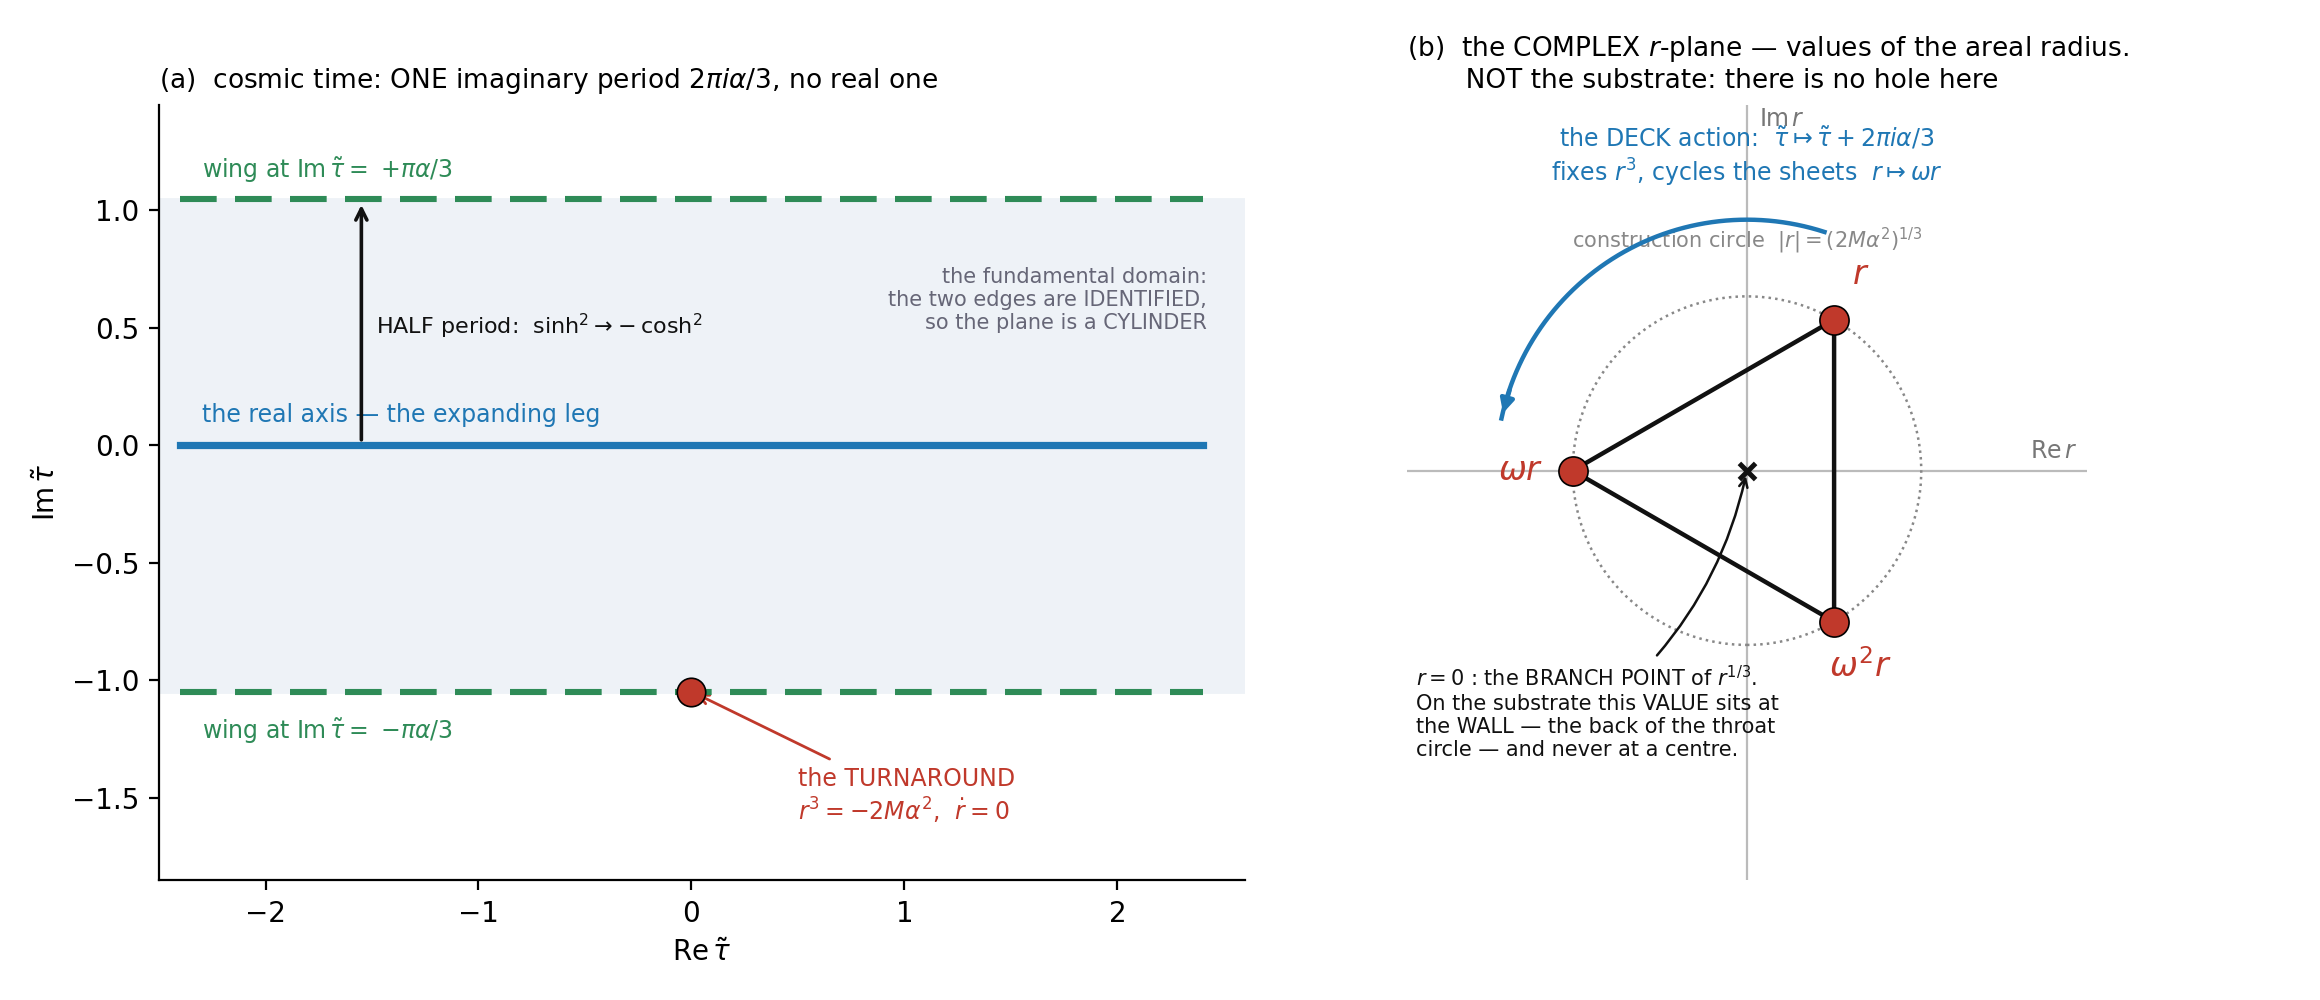
\includegraphics[width=\textwidth]{figures/CR_turnaround_threeness.png}
\caption{The construction's \emph{other} three-ness, and the contrast with Figure~\ref{fig:U3} is the point of drawing it.\rcpt{P03_the_turnaround_figure} \emph{(a)} The complexified cosmic-time plane of the bead's outward law $r^{3}=2M\alpha^{2}\sinh^{2}(3\tilde\tau/2\alpha)$. That law has \emph{one} imaginary period, $2\pi i\alpha/3$, and no real one, so the shaded band is a fundamental domain whose two edges are identified and the plane quotients to a cylinder---which is why everything here closes in elementary rather than elliptic terms. The half-period wings sit at $\mathrm{Im}\,\tilde\tau=\pm\pi\alpha/3$ and carry $\sinh^{2}\mapsto-\cosh^{2}$, the real expanding leg to the conjugate collapse law; the turnaround is the point $\tilde\tau=-i\pi\alpha/3$, where $r^{3}=-2M\alpha^{2}$ and the velocity vanishes together, so it is a turnaround in fact and not by label. \emph{(b)} The \emph{complex $r$-plane}---a plane of \emph{values} of the areal radius, and emphatically \emph{not} a picture of the substrate, so that nothing in it is a hole and its centre is not a place. The three cube-root sheets the deck action $\tilde\tau\mapsto\tilde\tau+2\pi i\alpha/3$ permutes: it leaves $r^{3}$ invariant and sends $r\mapsto\omega r$, and the three roots have one modulus with arguments spaced by exactly $120^{\circ}$---equilateral, the dotted circle being a construction circle of radius $(2M\alpha^{2})^{1/3}$ recording that equality and nothing more. \emph{The origin deserves its own sentence, since it is the one point of this figure that is easily mislocated on the other.} There $r=0$ is the branch point of the cube root, a \emph{value}; on the substrate that value sits at the \emph{wall}---the back of the throat circle, at $X_{1}=-\alpha$, a point \emph{on} the circle (\S\ref{sec:hinge-geometry})---and never at any centre, the interior of the throat carrying no manifold at all. \emph{The contrast with the hinge triple is total.} That three indexes the within-state label, carries the full Weyl $S_{3}$, lives in the equatorial section, and consists of \emph{roots} of the horizon cubic at radius $2\alpha$; this one indexes the family~\cite{JanzenMatter}, carries only the cyclic $\mathbb{Z}_{3}$ of the deck group, lives in complex cosmic time, and consists of \emph{sheets}. The companion framework paper's \emph{lem:twoturnings} establishes that no affine change of variable identifies the two root sets, so the two three-nesses are genuinely two, and reading a single figure as though it carried both is the error this pair of figures exists to prevent.}
\label{fig:turnaround}
\end{figure}

\subsection{The other three-ness, and where it differs on the inside}\label{sec:temporal-threeness}
The hinges above are a \emph{spatial} three-ness: three colinear-real horizon roots, permuted by $S_{3}$, designated by the offset. The family's other cubic carries a three-ness too---the comoving turnaround of Figure~\ref{fig:ellipse}, whose roots form an equilateral triangle---and the companion framework paper's \emph{lem:twoturnings} establishes that no affine change of variable identifies the two root sets. That is a separating statement. What the turnaround's three-ness positively \emph{is} can be said here, because it is read off the bead's outward law $r^{3}=2M\alpha^{2}\sinh^{2}(3\tilde\tau/2\alpha)$ and this paper owns the geometry it lives in.

It is the deck action of cosmic time's own imaginary period (Figure~\ref{fig:turnaround}). The shift $\tilde\tau\mapsto\tilde\tau+2\pi i\alpha/3$ leaves $r^{3}$ \emph{invariant} and permutes the three cube-root sheets cyclically, $r\mapsto e^{2\pi i/3}r$: the turnaround cubic's $\mathbb{Z}_{3}$ and that period are one object.\rcpt{P03_turnaround_temporal_threeness} The word \emph{period} is exact and is worth holding to its exact sense, and holding it
so answers a question the construction raises everywhere: why everything here closes in elementary terms. The
period is a \emph{single} one---$\sinh^{2}$ has the one period $i\pi$ in its argument, no real period, and none
with both parts nonzero---so the quotient of the $\tilde\tau$-plane by it is the cylinder
$\mathbb{C}/\langle 2\pi i\alpha/3\rangle\cong\mathbb{C}^{\times}$ and the law is a rational function of
$e^{3\tilde\tau/2\alpha}$\rcpt{X2r_single_periodicity}. That is the whole of it: a singly periodic meromorphic
function is elementary, a doubly periodic one is elliptic, and no elementary closed form exists for the second.
The same holds of the horizon side in its own variable, where $\sin 3w$ carries the single real period $2\pi/3$
(\S\ref{sec:tour})~\cite{JanzenGroupoid} and no imaginary one. \emph{Each of the construction's two three-nesses
is one singly periodic elementary function composed with a three-fold}---$\sinh^{2}$ with the cube root on the
turnaround side, $\sin$ with the triple angle on the horizon side---and that, not any convenience of
presentation, is why $\sinh^{2/3}$, $\sin 3w$ and the involution $\sigma$ all admit closed forms where a
doubly periodic structure would return elliptic functions in their place. The two periods moreover differ in kind
as the two three-nesses do: $2\pi i\alpha/3$ is purely imaginary, along the clock; $2\pi/3$ purely real, along the
dial. So where the horizon triple is the slicing's spatial three-ness, this is the \emph{temporal} one---not by analogy, but because its generator is a period of $\tilde\tau$.

Two consequences follow, and the second is the sharper. First, the half of that period does definite work: $\tilde\tau\mapsto\tilde\tau+i\pi\alpha/3$ carries $\sinh^{2}\mapsto-\cosh^{2}$ exactly, turning the real expanding leg into the conjugate collapse law $r=-(2M\alpha^{2})^{1/3}\cosh^{2/3}(3\operatorname{Re}\tilde\tau/2\alpha)$ on the negative branch. The two collapse wings at $\operatorname{Im}\tilde\tau=\pm\pi\alpha/3$ are therefore not placed by choice; they are the half-period images of the real leg. \emph{And that placement is what the companion papers then read, in two registers this paper does not enter.} The interval it fixes---the stretch at fixed $\operatorname{Re}\tilde\tau$ along which the areal radius climbs from the comoving turnaround to the branch point---is the \emph{lift}, and on it the conformal time is purely imaginary, so the areal rate is carried from zero at the turnaround to divergent at the branch point over no cosmic time at all: that is what supplies the initial expansion rate rather than postulating it~\cite{JanzenCRframework}. The same interval carries a marked locus this paper's geometry admits but does not name---the unit-speed point interior to the wing, at which the null condition $|\dd r/\dd s|=1$ is met for the third time on one lap, the two seam passes being the other two---so that the causal character of the whole excursion is well defined throughout. \emph{And the discrete skeleton classified here is the same object the description groupoid classifies algebraically}: the involution $\sigma$'s fixed point, proved there to be Nariai, is the seam the excursion crosses at unit speed \emph{without} a change of causal character, which is why the family's five spans carry only four distinct characters~\cite{JanzenGroupoid, JanzenCRframework}. \emph{This paper builds the geometry in which all three statements live; it makes none of them.} And the turnaround is not a point somewhere along a wing: at $\tilde\tau=-i\pi\alpha/3$ one has $\sinh^{2}=-1$ exactly, so $r^{3}=-2M\alpha^{2}$ and $r=-(2M\alpha^{2})^{1/3}$ with vanishing $\tilde\tau$-velocity. \emph{The kinematic turning is the half-period.}

Second, this is an asymmetry between the two three-nesses that runs deeper than their affine inequivalence. The temporal $\mathbb{Z}_{3}$ \emph{factors through} a half-period that exchanges the branches---matter leg to conjugate leg, $r>0$ to $r<0$. The spatial $S_{3}$ carries no exchange inside itself: $f=0$ is a condition on $r$ alone, carries no shift of $\tilde\tau$, and nothing within the permutation of its roots exchanges the branches. \emph{The asymmetry is one of where the exchange sits, not of whether one exists}---the spatial side has its branch exchange in $R$, which carries $r_{0}\mapsto-r_{0}$ and so maps the triple $(r_{N},r_{N},-2r_{N})$ to its $P$-conjugate twin $(-r_{N},-r_{N},2r_{N})$: an exchange \emph{between} the two Nariai members rather than inside one member's $S_{3}$. The temporal case differs precisely there, its exchange being internal to the $\mathbb{Z}_{3}$'s own generator. \emph{The two order-threes differ not only in how their roots sit but in what lives inside them.} What is \emph{not} claimed, here or anywhere in this paper: any identification of the two cubics' root sets, which the framework paper's order-three bridge holds open, and any reading of the turnaround triangle as a weight diagram---withdrawn as over-reach and not revived. The statement above concerns the interior of one three-ness, not a bridge between two.

One more thing the two seams do, and it is the $2{:}1$ again in a different variable. Read along the closed slicing in the phase $w=3c\tilde\tau/2\alpha$ of the bead's outward law, the front seam sits where $\sinh w=1/\sqrt2$ and the backward-radial root where $\cosh w=2$; since $\cosh 2w=1+2\sinh^{2}w$, the first of those is $\cosh 2w=2$, and therefore
\begin{equation}
  w_{\text{back}}=2\,w_{\text{front}}=\operatorname{arccosh}2=\ln(2+\sqrt3).
  \label{eq:seamphases}
\end{equation}
\emph{The $2{:}1$ the two roots carry in areal radius appears as a $1{:}2$ in phase, inverted}, and by an identity rather than a coincidence: the ratio enters the radii as $2^{-1/3}$ against $2^{2/3}$ and leaves the phases as a factor two, because one leg is read on $\sinh^{2/3}$ and the other on $\cosh^{2/3}$.\rcpt{P07_lap_timeline} \emph{What the phases are and are not:} $w$ is set by the proper time of the fundamental observers, so these are intervals of that clock and not of the exterior static one, in which no horizon completes at finite time~\cite{JanzenBHcausality,JanzenCRframework}.

One further thing follows once both cubics are on the table. That they meet at $r=0$ and nowhere else---$H-T=-\alpha^{2}r$, writing $H=r^{3}-\alpha^{2}r+2M\alpha^{2}$ and $T=r^{3}+2M\alpha^{2}$---is the framework paper's, where it does its work separating the two turnings as events~\cite{JanzenCRframework}. What can be added from this side is why their \emph{characters} separate, and it is a reason that is read off the discriminants and nothing else. $\operatorname{disc}H=-4\alpha^{4}(27M^{2}-\alpha^{2})$ \emph{can} vanish---it does, at the Nariai mass $M=\alpha/3\sqrt3$---and that is the double root, giving the ordered triple $(r_{N},r_{N},-2r_{N})$ with $r_{N}=\alpha/\sqrt3$: the merged front seam and the backward-radial root at twice its magnitude, the $2{:}1$ this paper reads off the ellipse's Nariai ordinate. $\operatorname{disc}T=-108M^{2}\alpha^{4}$, by contrast, is \emph{strictly negative for every} $M\neq0$ and so never vanishes: the turnaround's triple is equilateral always, its roots can never merge, and it contributes a single lone real point rather than a coincidence. \emph{The seam's ability to merge and the turnaround's inability to are the same fact seen twice}---the $-\alpha^{2}r$ that separates the cubics is exactly what gives $H$ a discriminant that can vanish, and its absence from $T$ is why $T$'s cannot.\rcpt{P03_cubic_spacing} So the flat term does double duty: it fixes where the two cubics meet, and it decides which of them can degenerate.

\section{The equatorial seam, the overcritical continuation, and the conjugate branch}\label{sec:seam}

The turning points of the slicing curve are the horizons---the zeros of $f$, where $\mathrm{d}r/\mathrm{d}l$ vanishes (Proposition~\ref{prop:turning}), read geometrically as the points at which the secant meets the throat circle. We call such a turning point a \emph{seam}, and we now show that the seam's explicit, invertible analytic continuation secures the de Sitter $\leftrightarrow$ Schwarzschild correspondence---witnessing the slicing's reversible membership in de Sitter---and that the continuation past the seam onto the backward-radial branch is what closes the slicing into a single object.

\subsection{The two pieces}

Near a turning point the slicing curve has a definite local form. Take the de Sitter slicing for concreteness, $r=\alpha\sin\theta$ with $\theta=l/\alpha$, and set $\alpha=1$. For $\theta\in[0,\pi/2]$ the curve rises from $r=0$ to the seam at $r=1$; the relevant two-dimensional line element is the round spherical one,
\begin{equation}\label{eq:sph}
  ds^{2}=d\theta^{2}+\sin^{2}\!\theta\;d\Omega^{2},
\end{equation}
of Riemannian signature $(+,+)$. At the seam $\theta=\pi/2$, $\sin\theta$ reaches its maximum and $d r/d\theta=\cos\theta$ vanishes: the curve is tangent to the throat circle.

\subsection{Continuation through the equatorial seam}

\begin{proposition}[Automatic signature flip]\label{prop:flip}
Under the analytic continuation $\theta\mapsto\pi/2+i\psi$, the spherical line element \eqref{eq:sph} becomes the de Sitter line element
\begin{equation}\label{eq:dscont}
  ds^{2}=-d\psi^{2}+\cosh^{2}\!\psi\;d\Omega^{2},
\end{equation}
of Lorentzian signature $(-,+)$.\rcpt{P03_seam_continuation} The signature flip is not imposed; it follows from $d\theta=i\,d\psi$.
\end{proposition}

\begin{proof}
Write $\theta=\pi/2+i\psi$. Then $d\theta=i\,d\psi$, so $d\theta^{2}=-d\psi^{2}$. And $\sin\theta=\sin(\pi/2+i\psi)=\cos(i\psi)=\cosh\psi$. Substituting both into \eqref{eq:sph} gives $ds^{2}=-d\psi^{2}+\cosh^{2}\psi\,d\Omega^{2}$, which is \eqref{eq:dscont}. The sign of the first term has changed because the continuation factor $i$ in $d\theta=i\,d\psi$ squares to $-1$; no signature change was inserted by hand.
\end{proof}

\begin{remark}[The seam is where two reality-lines of $\sin$ cross, at a critical point]\label{rem:reality-lines}
Proposition~\ref{prop:flip} and the tangency that defines a seam are one fact about $\sin$, and stating it
that way gives both, together with the $C^{1}$ join and the signature flip. Since
$\operatorname{Im}\sin(x+iy)=\cos x\,\sinh y$, the locus on which $\sin$ is real is a grid: the real axis
$y=0$, along which $r=\sin\theta$ is the spherical piece, together with the vertical lines
$x=\pi/2+k\pi$, along which $r=\cosh\psi$ is the Lorentzian one. \emph{The seam is where two of those lines
cross}, and the crossings are exactly the critical points of $\sin$, where $\cos$ vanishes\rcpt{X3r_reality_lines}.
Four properties follow from that single fact at once: $r$ is maximal there, because a critical point is where it
is; $\mathrm{d}r/\mathrm{d}\theta=0$, which is the tangency to the throat circle by which
\S\ref{sec:seam} \emph{defines} a seam; both pieces are real, because both crossing lines are reality-lines;
and the join is $C^{1}$, because the derivative vanishes along each. The signature flip is the same fact once
more: the two lines cross at right angles, so the increment turning from one onto the other is $i\,\mathrm{d}\psi$,
and a metric is of degree two, so $\mathrm{d}\theta^{2}=-\mathrm{d}\psi^{2}$ where a scalar would have carried
across unchanged. This is also where the substrate's everywhere-real character is met locally: the imaginary
variable is an instrument that lands the construction on a line where the same entire function takes real
values~\cite{JanzenGeometricCore}, and no continuation across a boundary is performed, $\sin$ being entire. The grid also sorts the de~Sitter member's own horizon triple by type. With $M=0$ the cubic is $r^{3}-\alpha^{2}r=0$, roots $\{+\alpha,0,-\alpha\}$; the crossings of the reality lines sit at $r=\pm\alpha$, alternately, while $r=0$ lies on the real axis away from any crossing\rcpt{C5_sct_already_linear}. So the two $R$-conjugate horizons are the points where two reality-lines meet and the branch point is the one lying on a single line---the alternation $+\alpha,-\alpha$ along the grid being the mass-reflection read on it.
\end{remark}

The two pieces---spherical \eqref{eq:sph} and de Sitter \eqref{eq:dscont}---are one analytic object. Since $\sin(\pi/2+i\psi)=\cosh\psi$, the function $r=\sin\theta$ continued from the real segment $\theta\in[0,\pi/2]$ onto the line $\theta=\pi/2+i\psi$ \emph{is} $r=\cosh\psi$. The seam $\theta=\pi/2$ is the \emph{join}: the point at which the parameter turns off the real axis into the imaginary direction, at $r=1$. Both pieces meet there at $r=1$ with vanishing first derivative: the join is $C^{1}$, the slicing curve tangent to the throat circle from both sides. Figure~\ref{fig:seam} shows the join.

\begin{figure}[t]
  \centering
  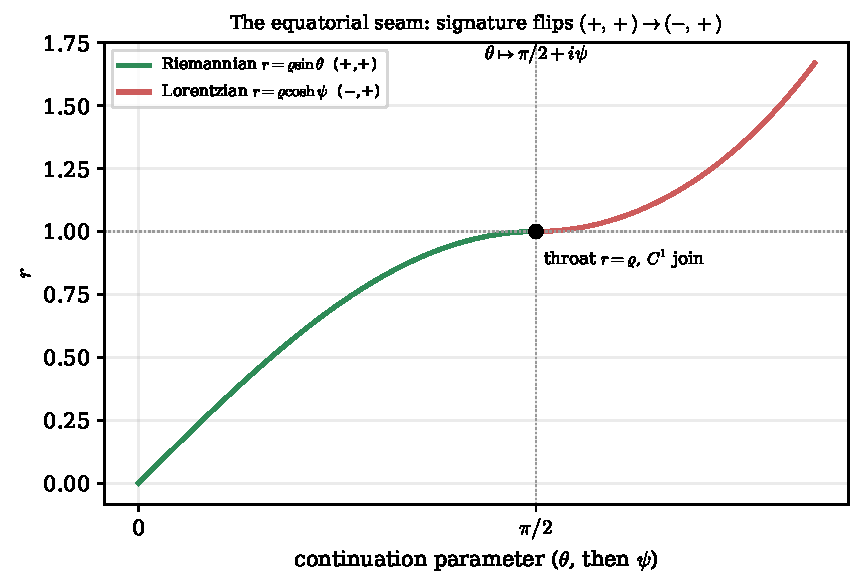
\includegraphics[width=0.78\textwidth]{figs/fig4_seam.pdf}
  \caption{The equatorial seam. The Riemannian spherical piece $r=\varrho\sin\theta$
  meets the Lorentzian dual piece $r=\varrho\cosh\psi$ at the throat radius $r=\varrho$.
  The two are one analytic function continued through $\theta\mapsto\pi/2+i\psi$;
  the join is $C^{1}$, and the metric signature flips from $(+,+)$ to $(-,+)$
  automatically, because $d\theta=i\,d\psi$ squares the continuation factor
  to $-1$.}
  \label{fig:seam}
\end{figure}

\subsection{The correspondence as a continuation}

The companion paper carried out exactly this continuation at the two critical points of the Schwarzschild cycloid: $z\mapsto i\rho$ at $z=0$ produced an exterior at $r>2M$ (a front-seam continuation), and $z\mapsto\pi+i\rho'$ at $z=\pi$ produced the back-seam continuation onto $r<0$, with the trigonometric functions of the interior becoming the hyperbolic functions of the exterior. Proposition~\ref{prop:flip} is the same operation, identified now as the join between a Riemannian and a Lorentzian piece of one slicing curve. The signature that flips here is that of this two-dimensional slicing-surface metric: the radial direction the curve runs along reads spacelike on the spherical (hole-side) piece $r<\alpha$ and timelike on the de~Sitter (cosmological) piece $r>\alpha$, flipping as the curve crosses the throat. It is not the signature of the spacetime, which is Lorentzian throughout---the substrate is one Lorentzian manifold, and the continuation relates two real regions of it, never carrying the geometry off the real Lorentzian substrate onto a Euclidean one. This is worth marking against the distinct continuation the substrate also admits, and with which it must not be run together: the \emph{global} Wick rotation $x_{0}\mapsto ix_{0}$ does carry the whole Lorentzian substrate onto its conjugate real form---the compact $S^{5}=\mathrm{SO}(6)/\mathrm{SO}(5)$, the two of them the real forms of the one complex group $\mathrm{SO}(6,\mathbb{C})$---on which a continuous $\mathfrak{su}(3)$, colour's, lives~\cite{JanzenBoundary,JanzenGeometricCore}. The seam continuation is not that operation: it is real-analytic, joining two real regions of one Lorentzian geometry (the slicing surface's Riemannian$\leftrightarrow$Lorentzian seam), where the global Wick carries the substrate to its \emph{other real form} entirely (a Lorentzian$\leftrightarrow$Euclidean move). Colour therefore sits on the substrate's own conjugate face, reached by a continuation the slicing never performs---the two continuations distinct in kind, and conflating them the characteristic error the coupling guards against.

This secures the de Sitter $\leftrightarrow$ Schwarzschild correspondence in concrete form. A slicing built by running $\sin\theta$ out to the equatorial seam and continuing onto $\cosh\psi$ can be run backwards, because $\sin$ and $\cosh$ are one analytic function and the continuation $\theta\mapsto\pi/2+i\psi$ is invertible. The inverse is not a separate construction to be discovered: it is guaranteed by the analyticity of the continuation. A geometry obtained as a slicing of de Sitter retains, in the invertibility of that slicing, its membership in de Sitter. The cosmological-side continuation here---the Lorentzian de~Sitter piece $r>\alpha$ onto which the slicing opens---is the geometric substrate of the cosmogenesis developed in the cosmological completion~\cite{JanzenCRframework}, where the reading of the branch-point crossing as the reassignment of the radial direction to cosmic time is taken up; it is not asserted here.

\subsection{Overcritical SdS: the same continuation past the Nariai crest}\label{sec:overcritical}

The undercritical/overcritical boundary of Section~\ref{sec:ellipse}, $|2M|=2/(3\sqrt{3})$, is in the sky angle of Section~\ref{sec:throat-angle} the crest of $\sin(3w)$. Overcritical SdS is reached by the same analytic continuation as the seam, applied now to the horizon angle itself.\rcpt{P03_overcritical}

By Proposition~\ref{prop:triple}, $2M=\tfrac{2}{3\sqrt3}\sin(3w)$. The overcritical range $|2M|>2/(3\sqrt3)$ requires $|\sin(3w)|>1$, impossible for real $w$. Writing $3w=\pi/2+i\beta$ gives $\sin(3w)=\cos(i\beta)=\cosh\beta>1$: the horizon angle is continued off the real axis into the imaginary direction, exactly as $\theta\mapsto\pi/2+i\psi$ at the seam. The Nariai crest $3w=\pi/2$ is the Nariai point. Overcritical SdS is thus not a separate construction; it is the slicing of Sections~\ref{sec:slicing}--\ref{sec:ellipse} with the horizon angle continued past the Nariai crest, and the same $\sin\to\cosh$ mechanism that joins the Riemannian and Lorentzian pieces of the seam carries the geometry from the under- to the over-critical regime.

\paragraph{The root structure, read off the locus.} The overcritical regime is read directly off the horizon locus of Section~\ref{sec:ellipse} with no separate algebra. That locus is the diagonal $r=r_{0}$ together with the tilted ellipse $r^{2}+r r_{0}+r_{0}^{2}=1$, and the three horizons at a given slicing are the intersections of the vertical line at fixed $r_{0}$ with this locus. For $|r_{0}|<2/\sqrt{3}$ the line meets the ellipse in two real points and the diagonal in one: three real roots. At $|r_{0}|=2/\sqrt{3}$ the line is tangent to the ellipse: the double root, Nariai. For $|r_{0}|>2/\sqrt{3}$ the line misses the ellipse in the real plane and meets only the diagonal: one real root, together with the complex-conjugate pair arising as the intersection with the \emph{analytic continuation} of the same fixed ellipse into the complex $(r,r_{0})$ plane. The ellipse does not disappear in the overcritical regime; the real slicing line simply ceases to meet it, and the two horizons continue, as a conjugate pair, on the ellipse's complex extension. This is the same continuation as the seam, now seen in the $(r,r_{0})$ plane: $\sin\to\cosh$ at the seam, loss of real intersection here, one analytic fact in two guises.

The sign of the surviving real root follows from the diagonal. By Proposition~\ref{prop:factor} the diagonal root is $r_{0}$ itself, and $2M=r_{0}-r_{0}^{3}$; for $2M>2/(3\sqrt3)$ the real root lies at $r_{0}<0$, and for $2M<-2/(3\sqrt3)$ at $r_{0}>0$---the overcritical real horizon is the backward-radial root, the one carried by the major axis of the ellipse (Section~\ref{sec:ellipse}).

\paragraph{The symmetry action, continued.} The root-exchange continues with the geometry, stating the overcritical symmetries the locus above leaves implicit. In the sky angle $\sigma$ is the reflection $w\leftrightarrow\pi/3-w$ (Section~\ref{sec:throat-angle}); at the overcritical angle $w=\pi/6+i\beta/3$ it acts as $\sigma(w)=\pi/6-i\beta/3=\bar w$---\emph{complex conjugation}---so it exchanges the conjugate pair of horizons and fixes the surviving real backward-radial root, exactly as it exchanges the two real roots and fixes the third undercritically. The one involution thus acts across the Nariai crest at its fixed point $w=\pi/6$, swapping a real pair below and the conjugate pair above; and the backward-radial reflection $r_{0}\mapsto-r_{0}$ (the outer $\mathbb{Z}_{2}$) carries between the two sign-halves overcritically as under. The full $\mathrm{Aut}(A_{2})=S_{3}\times\mathbb{Z}_{2}\cong D_{6}$ is therefore the symmetry of the overcritical regime no less than the undercritical, realised there on the complex-conjugate root structure. This regime-dependent realisation---all of $S_{3}$ on the three real roots undercritically, only the order-two complex conjugation of the pair overcritically---is read off the slicing here; the companion groupoid paper carries it onto the description foliation and casts it group-theoretically, as the monodromy group of the branched cover~\cite{JanzenGroupoid}.

\paragraph{The slicing curve in the overcritical regime.} It remains to carry the slicing curve itself, $dr/dl=\sqrt{|f(r)|}$, through the continuation. The defining equation does not refer to the number of real roots of the cubic; it is well defined wherever $f$ is, and $f(r)=1-2M/r-r^{2}/\alpha^{2}$ is real for real $r$ whatever the value of $2M$. The analytic continuation parametrises $r_{0}$ through a complex sky angle---from $r_{0}=\tfrac{2}{\sqrt3}\sin w$ with $w=\pi/6+i\beta/3$, $r_{0}=\tfrac{2}{\sqrt3}\bigl(\tfrac12\cosh\tfrac{\beta}{3}+i\tfrac{\sqrt3}{2}\sinh\tfrac{\beta}{3}\bigr)$---but the curve $r(l)$ it labels remains real: $r_{0}$ is an algebraic label of the slicing, while the physical curve runs through real radial values.

On the forward branch $r>0$ the overcritical $f$ has no zero at all: with $2M$ past the Nariai value, $f(r)<0$ for every $r>0$, so $dr/dl=\sqrt{|f|}$ never vanishes there. The forward slicing curve therefore has \emph{no} turning point---it is unbounded, with a single real turning point present only on the backward branch, at the negative root identified above. This is the precise overcritical statement of the turning-point correspondence: of the three horizons, one survives as a real turning point of the curve (on the backward branch) and two have left the real slice as the conjugate pair on the continued ellipse.

The asymptotic form of the unbounded forward curve follows at once. For large $r$, $f(r)\to-r^{2}/\alpha^{2}$, so $dr/dl\to r/\alpha$ and
\begin{equation}\label{eq:overcrit-asymp}
  r(l)\sim e^{\,l/\alpha},
\end{equation}
an exponentially growing branch---the global continuation of the same hyperbolic ($\cosh$) piece that the seam construction initiates locally.

\subsection{The lap and the conjugate branch}\label{sec:lap}

The negative-root horizon of Section~\ref{sec:ellipse} and the backward-radial real root of the overcritical regime are the same structure, and naming it correctly closes the slicing into a single object. The areal radius $r$ is a \emph{signed} coordinate: the angular part of \eqref{eq:sds} is $r^{2}\,d\Omega^{2}$, so $g_{\theta\theta}=r^{2}$ is insensitive to the sign of $r$, and the curve may be run in the negative sense---the backward radial direction, the long way round from $r=0$---without leaving the geometry. The major axis of the locus ellipse (Section~\ref{sec:ellipse}) is precisely this backward-radial direction $r=-r_{0}$, and the third root the factorisation \eqref{eq:factored} always supplies lives on it.

This is what lets the slicing close. Ride the curve inward along a ruling to the equatorial seam; continue, by Proposition~\ref{prop:flip}, around the throat through $r=0$ and out onto the negative branch; and the curve closes on the backward-radial root carried by the major axis. The point $r=0$ on this lap is the branch point at which the real radial value passes between the forward ($r>0$) branch and the backward ($r<0$) branch---the same branch point the companion paper reached by $z\mapsto\pi+i\rho'$ at the conjugate critical point of the cycloid~\cite{JanzenCircle}. It is not a barrier. The substrate is the one smooth de Sitter manifold, which is $C^{\infty}$ across the locus the chart labels $r=0$; the divergence of the curvature \emph{reading} there (Section~\ref{sec:curvature}) is a property of the perspectival areal coordinate, the same chain-rule artefact the companion paper identified~\cite{JanzenCircle}, not of the manifold.

The region reached on the backward branch is therefore the \emph{conjugate} region: the real $r<0$ branch of the one Lorentzian substrate, continued through the $r=0$ branch point. It is not a Euclidean excursion---the signature flip of Section~\ref{sec:seam} is that of the two-dimensional slicing surface, and the spacetime is Lorentzian throughout---and the conjugate horizons of the overcritical regime are its complex shadow on the fixed ellipse, the genuine backward-radial root its real representative. The slicing curve, run forward through the seam and backward through $r=0$, is one closed object on one manifold; the horizon, the curvature-singularity reading, and the cosmological horizon are its turning points, forward and backward.

Read against the linearly-marching areal radius, the lap is oscillatory where the real legs are monotone. On the real ruling legs the embedding coordinate $X_{1}=\alpha\cos\theta$ is linear in $r$; around the conjugate lap, where $r$ marches as arc length through the three roots $+\alpha/\sqrt3,\,0,\,-2\alpha/\sqrt3$, it traces a single cosine arch, troughing at $r=0$ (the back of the throat circle, $X_{1}=-\alpha$) and closing the lap at the backward-radial root (Fig.~\ref{fig:conjwave}). This is a property of the embedding coordinate read against the signed areal radius, not of the metric, which is regular across the lap as established above.

Read forward as physics rather than geometry, the lap is the \emph{cosmogenesis}: the conjugate branch is a previous universe's collapsed matter continued through the seam, its completion read by the framework as our own expanding cosmology---the two the framework proves one closed \emph{cosmogenetic bead}, the curve established here its geometric skeleton~\cite{JanzenCRframework}---so that the primordial light-element abundances become a fossil of that collapse's thermal history---the quantity the companion cosmogenesis paper computes, and the loop this slicing opens by carrying the curve through $r=0$ is the loop it closes~\cite{JanzenCosmogenesis}. This single curve is the geometric skeleton of the cosmology's layered reading: read \emph{inward} it is the collapsing leaf's own self-gravitating dynamics---the local rate, its content gravitating, where the light elements freeze out---and read \emph{outward} it is the observable foliation's geometry-set stacking rate, the two being one congruence crossing the one seam rather than two regimes, exactly as the marginally-bound cosmological geodesic is dust collapse read inward and dust cosmology read outward~\cite{JanzenCRframework, JanzenCosmogenesis}. And the member the framework's reassignment installs is fixed here, geometrically and not by fitting: it is Nariai, the one fixed point of the root-exchange involution~\eqref{eq:involution}, at which the two horizons the curve turns on merge.

\begin{figure}[t]
    \centering
    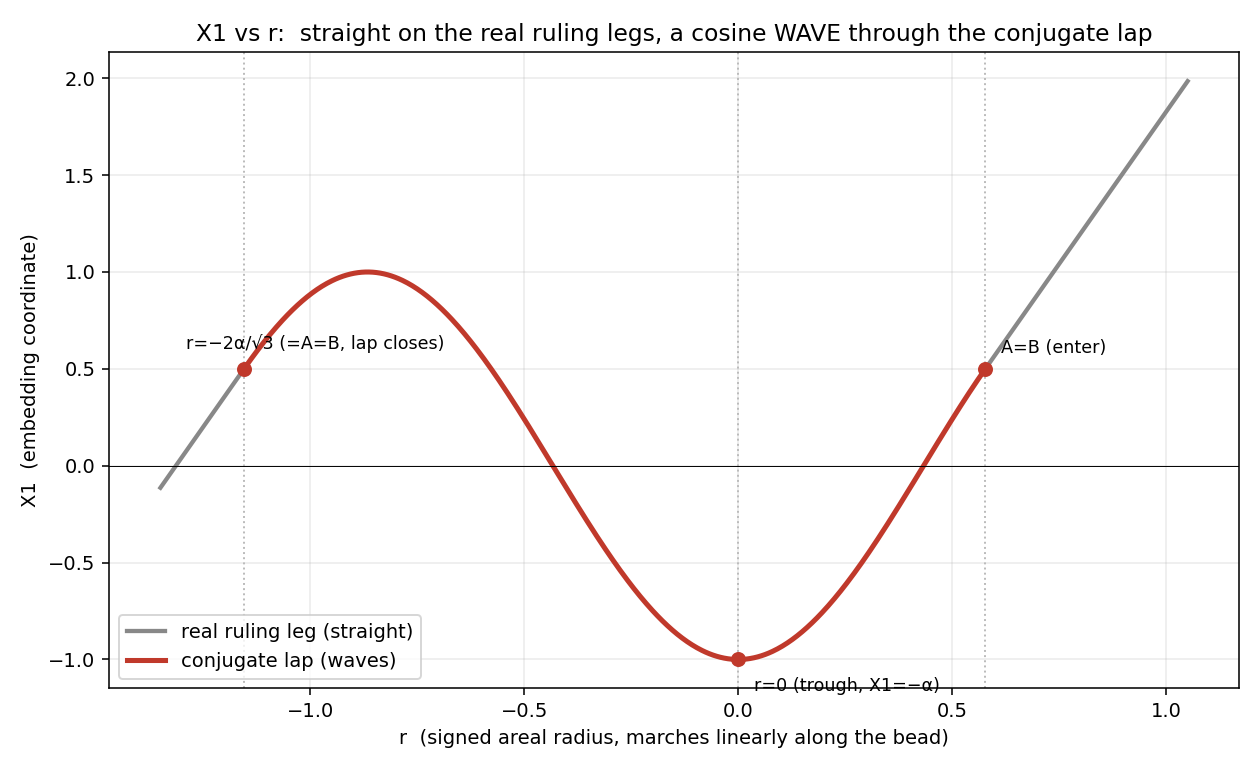
\includegraphics[width=0.62\textwidth]{X1_vs_r_conjugate_wave.png}
    \caption{The lap of this section, plotted as the embedding coordinate $X_{1}=\alpha\cos\theta$ against the signed areal radius $r$ (read as arc length along the bead). On the real ruling legs (grey) $X_{1}$ is linear in $r$; around the conjugate lap (red) it traces a single cosine arch, troughing at $r=0$ (the back of the throat circle, $X_{1}=-\alpha$) and closing at the backward-radial root $-2\alpha/\sqrt3$, the merged-horizon value re-entered. The oscillatory character belongs to the conjugate lap; the real legs are monotone.}
    \label{fig:conjwave}
\end{figure}

\subsection{Winding on the equator, and the thirds that closure forces}\label{sec:winding}

The lap of Section~\ref{sec:lap} is a closed circuit, and a closed circuit admits a count. Section~\ref{sec:tour} placed three graze points on the throat at polar $60^{\circ}$, $180^{\circ}$ and $300^{\circ}$, one directly between each pair of hinges, cutting the throat circle into three equal arcs; those are the only marked points the throat carries, and there are exactly three of them because there are three hinges. \emph{Define a constituent's winding as the signed number of graze points its equatorial route crosses, in units of one third of a lap.}\rcpt{P03_thirds_from_closure} Nothing further is stipulated.

One fact about routes then does all the work. Between two punctures at different hinges there are exactly two equatorial routes, and they cross one and two graze points in opposite senses; since $1+2=3$, \emph{the two routes differ by exactly one lap}. So a triple built on the three hinges has a head carrying some winding $x$ and two partners carrying $y$, with $x-y=1$ forced by that difference and nothing else.

Impose now only that the configuration \emph{close}---that a bound triple return to the branch it started on---for each of the two horn-headed arrangements. The upper-headed total is $x+2y$ and the lower-headed total is $y+2x$, and substituting $y=x-1$ these are $3x-2$ and $3x-1$. Both are integers precisely when $3x$ is, so
\begin{equation}\label{eq:thirds}
x=\tfrac{k}{3},\qquad k\in\mathbb{Z},
\end{equation}
and \emph{the thirds are forced rather than matched}---the $3$ being the number of constituents, of hinges and of graze points, which is one three entering three ways. Modulo a lap there are exactly three classes, and they are not assigned:
\[
k=2:\ \left(+\tfrac23,\,-\tfrac13\right),\qquad
k=1:\ \left(+\tfrac13,\,-\tfrac23\right),\qquad
k=0:\ \left(0,\,-1\right),
\]
the second being the first under overall sign---which is the charge conjugation of Section~\ref{sec:charge}---and the third the triality-zero class, carrying no fractional part at all. \emph{No Standard Model input enters the derivation}; what enters is the hinge count, the two-route fact and closure.

The horn swap is then a lap. The upper-headed triple of the $k=2$ class totals $\tfrac23-\tfrac13-\tfrac13=0$ and the lower-headed one totals $-\tfrac13+\tfrac23+\tfrac23=+1$, so \emph{exchanging the horns costs exactly one lap}, and the two closed arrangements form a doublet---with three of each, because there are three hinges.\rcpt{P03_winding_and_closure} Reading the fractional part and the integer part separately: the fractional part distinguishes the two conjugate classes, being $\tfrac23$ one way round the equator against $\tfrac13$ the other, and the integer part distinguishes the two members of a closed doublet, being one lap.

\emph{Closure is not an added rule, because the winding's transformation law is already the corpus's.}\rcpt{P03_sheet_index_and_factors} The areal radius on the lap is a cube root of an invariant---$r^{3}=2M\alpha^{2}\sinh^{2}(3\tilde\tau/2\alpha)$, the bead's law---and Section~\ref{sec:temporal-threeness} derives from cosmic time's single imaginary period that the deck action $\tilde\tau\mapsto\tilde\tau+2\pi i\alpha/3$ sends $r\mapsto e^{2\pi i/3}r$. So $r$ carries a sheet index in $\mathbb{Z}_{3}$ which advances by one at each passage through the $r=0$ branch point and returns after three: exactly the transformation law of a crossing count, obtained for reasons that have nothing to do with charge and before any of this was asked. \emph{To close is therefore to return to the same branch}, and admitting a composite exactly when its total fractional part vanishes is a statement about the covering rather than a selection rule imposed on it.

Read against the observed hadrons the rule agrees on every content tested: meson, baryon, antibaryon, tetraquark, pentaquark and dibaryon close and exist; a free quark, a diquark, $q\bar q q$, $qqqq$ and $qqq\bar q$ do not close and do not.\rcpt{P03_winding_and_closure} \emph{Confinement on this reading is a failure to close the lap}, and the closed lap is the object the construction admits as a slicing at all.

\emph{The scope is exact and is the same one Section~\ref{sec:charge} already draws.} What the geometry fixes is the \emph{quantisation}---that charge comes in thirds, and which classes exist---together with the sign, through $R$. It fixes no \emph{strength}: a topological label quantises and cannot scale, and the coupling is not in this construction. And the classes are read here as a combinatorial structure of the lap; that the $k=2$ class \emph{is} the quark doublet is a correspondence stated at the weight the companion matter paper states it, not a derivation of the Standard Model's content from this figure~\cite{JanzenMatter}.

\section{The curvature, the two sweeps, and the mass}\label{sec:geometry}

\subsection{The intrinsic curvature of the slicing surface}\label{sec:curvature}

The slicing curve, swept through one angular direction, generates a surface of revolution with line element $ds^{2}=dl^{2}+r(l)^{2}d\phi^{2}$, $l$ the proper radial distance. Its intrinsic curvature is a direct computation, and it is regular throughout the interior.

\begin{proposition}[Intrinsic curvature]\label{prop:curvature}
The slicing surface $ds^{2}=dl^{2}+r(l)^{2}d\phi^{2}$ has Gaussian curvature
\begin{equation}\label{eq:KG}
  K_{G}=-\frac{f'(r)}{2r}=\frac{1}{\alpha^{2}}-\frac{M}{r^{3}} .
\end{equation}
\end{proposition}

\begin{proof}
For a surface of revolution $ds^{2}=dl^{2}+r(l)^{2}d\phi^{2}$ the Gaussian curvature is $K_{G}=-r''(l)/r$. From $dr/dl=\sqrt{|f|}$, differentiating once more gives $r''(l)=\tfrac12 f'(r)\operatorname{sgn}f$ (as in the proof of Proposition~\ref{prop:turning}); on the static region $f>0$ this is $r''=\tfrac12 f'$, so $K_{G}=-f'/(2r)$. With $f'(r)=2M/r^{2}-2r/\alpha^{2}$ this is $K_{G}=1/\alpha^{2}-M/r^{3}$.
\end{proof}

Three consequences follow, and together they close the question of the interior. First, $K_{G}=1/\alpha^{2}-M/r^{3}$ is finite and smooth for every $r>0$: the slicing surface is regular throughout the static region between the horizons. The sole divergence is the $M/r^{3}$ pole as $r\to0$---the Schwarzschild curvature singularity of the companion paper~\cite{JanzenCircle}---and it is absent when $M=0$, where \eqref{eq:KG} reduces to the constant $K_{G}=1/\alpha^{2}$ of de Sitter.

Second, the curvature does not detect the horizons. At a horizon $r_{h}$, where $f(r_{h})=0$, the curvature $K_{G}(r_{h})=1/\alpha^{2}-M/r_{h}^{3}$ is simply a finite number; it neither diverges nor vanishes nor spikes there. The horizon is invisible to the intrinsic curvature---the precise statement, for SdS, that the horizon is a metric and chart feature and not a curvature feature, exactly as the companion paper found for Schwarzschild~\cite{JanzenBHcausality}.

Third, the curvature changes sign once, at
\begin{equation}\label{eq:rflat}
  r_{\mathrm{HE}}=(M\alpha^{2})^{1/3},
\end{equation}
being negative for $r<r_{\mathrm{HE}}$ and positive for $r>r_{\mathrm{HE}}$.\rcpt{P03_curvature_signflip} The slicing surface is therefore Schwarzschild-like (negatively curved, mass-dominated) in an inner region and de Sitter-like (positively curved, $\Lambda$-dominated) in an outer region, with the crossover at $r_{\mathrm{HE}}$. This crossover radius is a distinct locus from the horizons---the horizons are the zeros of $f$, the crossover is the zero of $f'$---and the zero of $f'$ carries a standard physical meaning: it is the \emph{static radius} of Schwarzschild--de~Sitter, the radius $r_{\mathrm{HE}}=(M\alpha^{2})^{1/3}$ at which the inward gravitational attraction $M/r^{2}$ and the outward cosmological repulsion $r/\alpha^{2}$ exactly balance, so that a static observer there feels no radial acceleration. The intrinsic curvature of the slicing surface therefore changes sign precisely at the classical gravitational--cosmological balance point---mass-dominated (Schwarzschild-like, negatively curved) within it, $\Lambda$-dominated (de~Sitter-like, positively curved) without. This locus lies between the two positive horizons, inside the static region (Figure~\ref{fig:curvature}). The curvature structure and the horizon structure are independent features of the same surface.

This crossover carries a physical reading the wider construction turns to account, worth drawing out here and developed on the theory in the companions. The two terms of $K_{G}$ are not on the same footing: $1/\alpha^{2}$ is the substrate's own de~Sitter curvature---the global, cosmological term set by $\Lambda$---while $-M/r^{3}$ is the local bend the mass adds, so $K_{G}$ is \emph{cosmological curvature minus local bend}, and the flat locus $K_{G}=0$ at $r_{\mathrm{HE}}$ is exactly where the local bend cancels the substrate's cosmological curvature. That locus has a standard name and use: the static radius $r_{\mathrm{HE}}=(M\alpha^{2})^{1/3}$ is the \emph{Hubble--Eddington radius}~\cite{Eddington1933}, $R_{\mathrm{TA,max}}=(3GM/\Lambda c^{2})^{1/3}$, the largest shell around a mass $M$ that can stay gravitationally bound against the cosmological expansion---within it a test particle falls inward, beyond it joins the Hubble flow---proposed as a \emph{local}, per-structure test of $\Lambda$ from the largest bound structures, robust to cosmic epoch, dark-matter details, and baryonic effects~\cite{PavlidouTomaras2014}. In the layered reading this boundary between a structure's gravitational hold and the cosmological flow is not a force cancellation computed after the fact but the \emph{intrinsic geometry of the existent slice}: mass-dominated and negatively curved (Schwarzschild-like, bound) within $r_{\mathrm{HE}}$, $\Lambda$-dominated and positively curved (de~Sitter-like, expanding) beyond it, the boundary appearing per structure and locally as the vanishing of the slicing surface's own Gaussian curvature---the local bend of the cut exactly cancelling the substrate's cosmological curvature. Its standing is a derivation and an explanation, not a re-description. The Hubble--Eddington radius, \emph{proposed} from the equation of motion of a test shell, is reached here independently as the flat locus of the existent slice, and under the layered ontology explained one level deeper: the boundary is where the real evolving space is intrinsically flat, its curvature-sign \emph{is} the boundedness/expansion dichotomy, and the test-particle balance is a consequence of that geometry rather than its definition. The value is general relativity's with $\Lambda$---necessarily, the framework leaving Einstein's equations untouched---so it discriminates no cosmology; the advance is the account, as sound as the layered ontology the programme holds to its tests. Gathered with the framework's other dissolutions, this boundary is one of the standing problems that paper's first synthesis resolves by the single distinction between the evolving existent and its maximally extended representation~\cite{JanzenCRframework}, and the epistemic discipline weighs the convergence of its several descriptions on one existent fact as one of its own assessments---the discipline returning a novel consequence, not merely certifying one~\cite{JanzenShadowExistence}. One scope stays honest: $K_{G}$ is the curvature of the two-dimensional slicing surface: carrying the reading to the full existent leaf and the actual bound dynamics---where matter is the bend of the cut~\cite{JanzenOperator} across the sector the substrate reaches~\cite{JanzenRange}, and the cosmological term is the substrate's own $\Lambda$-set expansion rate~\cite{JanzenCRcosmology}---is developed on the theory in those companions rather than on the surface alone; the static radius itself is the idealized spherical vacuum-exterior maximum, an upper bound to which virialization and the dark sector add the rest.
There is a second reading of the same locus, and it is an identity rather than a coincidence. Writing $f=1-2M/r-r^{2}/\alpha^{2}$ for the metric function, $f'=2M/r^{2}-2r/\alpha^{2}$ and $K_{G}=1/\alpha^{2}-M/r^{3}$ satisfy $K_{G}=-f'/2r$ identically; the factor never vanishes for $r>0$, so \emph{the flat locus of the slice and the stationary locus of the metric function are one locus, not two that agree}.\rcpt{P03_kg_is_fprime} The framework paper reads that same radius on the lap, where it is where the re-expansion is slowest~\cite{JanzenCRframework}---so the Hubble--Eddington radius \emph{is} the rate minimum, for every member, and the two characterisations were never independent. And the identity says more than that the loci agree. On any comoving worldline of the energy family $(\mathrm{d}r/\mathrm{d}\tilde\tau)^{2}=E^{2}-f$, so differentiating gives $\mathrm{d}^{2}r/\mathrm{d}\tilde\tau^{2}=-f'/2=rK_{G}$ exactly: \emph{the comoving acceleration is the slice's own Gaussian curvature, up to the positive factor $r$}. The sign of the intrinsic curvature of the existent slice \emph{is} the sign of the cosmic acceleration---negatively curved while the expansion decelerates, flat at the turnover, positively curved while it accelerates---so the flat locus this section identifies is not merely where a structure's hold balances the expansion but the epoch at which the expansion changes sign of acceleration.\rcpt{P03_acceleration_is_slice_curvature} On the Nariai member that locus is the seam, and in the standard reckoning it is where $\rho_{m}=2\rho_{\Lambda}$: the same condition, since $\rho_{m}/\rho_{\Lambda}=\operatorname{csch}^{2}(3c\tilde\tau/2\alpha)$ equals $2$ exactly at $\sinh=1/\sqrt2$, the seam's phase. \emph{It is therefore a recent, cosmological epoch rather than an early one}---and it precedes matter--$\Lambda$ equality, which sits later at $\sinh=1$.

One member of the family reads that boundary differently, and the difference is forced rather than coincidental. The condition $K_{G}=0$ is $M/r^{3}=1/\alpha^{2}$, and substituting it into the potential gives $f=1-3r^{2}/\alpha^{2}$: \emph{on the flat locus the mass term is absorbed and $f$ takes the pure de~Sitter form at scale $\alpha/\sqrt3$}. So $f(r_{\mathrm{HE}})=0$ holds precisely when $r_{\mathrm{HE}}=\alpha/\sqrt3$, which is $27M^{2}=\alpha^{2}$---the vanishing of the horizon cubic's discriminant. \emph{The Hubble--Eddington radius lies on a horizon for exactly one member of the family, and it is the double-root member}: below it $f(r_{\mathrm{HE}})>0$ and the crossover sits strictly inside the static region, as Figure~\ref{fig:curvature} shows for the undercritical case; above it $f(r_{\mathrm{HE}})<0$.\rcpt{P03_rstar_merged_horizon} At the degenerate member itself $r_{\mathrm{HE}}=r_{N}=\alpha/\sqrt3$, the merged horizon of Figure~\ref{fig:ellipse}'s Nariai ordinate---so there the boundary between a structure's gravitational hold and the cosmological flow \emph{is} the geometry's own horizon, and the amplitude $2^{1/3}r_{N}$ of that caption is $2^{1/3}r_{\mathrm{HE}}$, which is the ratio the abstract records. The same radius carries a third reading on the closed slicing: it is the lap's unique inflection, where the signed radius advances at unit rate against arc length~\cite{JanzenCRframework}. \emph{What is not claimed: nothing here bears on \emph{why} the cosmological reassignment selects the degenerate member---that selection is the framework paper's trichotomy and stands on its own. The statement is that the member so selected is the one whose structure-formation boundary coincides with its own merged horizon.}

\begin{figure}[t]
  \centering
  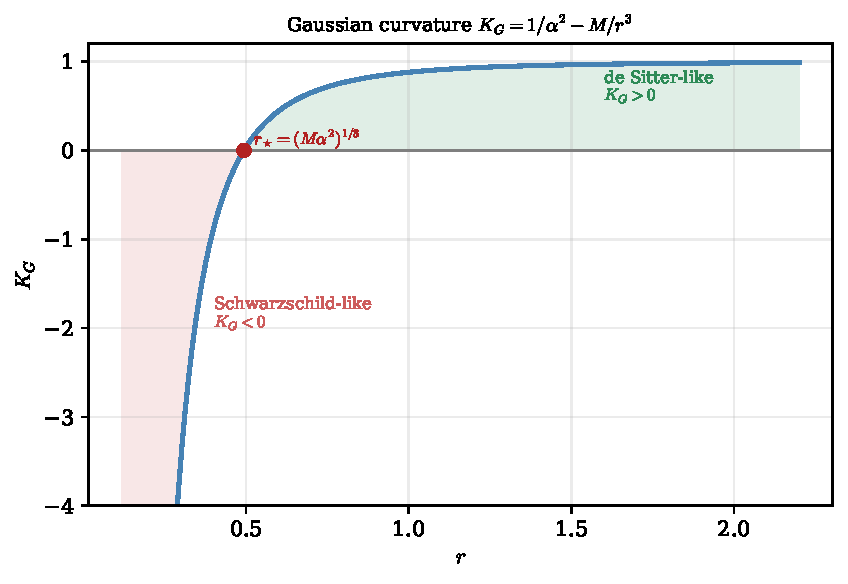
\includegraphics[width=0.74\textwidth]{figs/fig7_curvature.pdf}
  \caption{The intrinsic Gaussian curvature of the slicing surface,
  $K_{G}=1/\alpha^{2}-M/r^{3}$, across the static region (undercritical SdS,
  gauge $\alpha=1$). The curvature is finite and smooth throughout; it neither
  diverges nor vanishes at the two horizons. It changes sign once, at
  $r_{\mathrm{HE}}=(M\alpha^{2})^{1/3}$, between a Schwarzschild-like negatively
  curved inner region and a de Sitter-like positively curved outer region.
  The crossover radius $r_{\mathrm{HE}}$ is distinct from the horizons and lies
  between them.}
  \label{fig:curvature}
\end{figure}

\subsection{Schwarzschild and de Sitter as two sweeps}\label{sec:two-descriptions}

The de Sitter $\leftrightarrow$ Schwarzschild correspondence of Section~\ref{sec:seam} is \emph{one slicing curve swept from two vantages}. It must be held apart from a different operation, taken up in Section~\ref{sec:groupoid}: changing the observer who \emph{charts} a fixed swept geometry, under which the geometry is rigid (Proposition~\ref{prop:rigidity}) and only its image moves. The correspondence here is the other thing entirely---the same curve generating two geometries, because it is swept from two vantages. Swept from the interior vantage---about the manifold's own axis of symmetry, the hyperbolic section that is the worldline of the observer at $r=0$, the equatorial ring wrapping the radial direction in stationary coordinates---the curve generates the dynamical de Sitter geometry. Swept from the exterior vantage, viewing the hole from outside (Section~\ref{sec:sweep}), the causal roles of $r$ are flipped---$r$ is timelike along the equatorial interval between the horizon and $r=0$---and the same curve generates the static Schwarzschild geometry. It is the seam's automatic signature flip (Proposition~\ref{prop:flip}) that carries the one sweep into the other, turning the Riemannian spherical piece into the Lorentzian de Sitter piece without altering the curve itself. The two geometries are genuinely different geometries; the curve they are swept from is one. The whole Schwarzschild--de Sitter family is the exterior sweep taken across the slicing curves of Section~\ref{sec:projection}; de Sitter is the interior sweep.

This is the loop of the paper closed. Section~\ref{sec:seam} established the correspondence as an analytic continuation, structurally invertible; the present section identifies what that invertibility \emph{is}---the one slicing curve swept from two vantages, the interior and the exterior sweep carried into one another by the seam's signature flip, invertible because $\sin$ and $\cosh$ are one analytic function (Section~\ref{sec:seam}) and the curve itself is untouched by the flip. This is a different move from the charting-observer morphisms of the rigidity groupoid (Section~\ref{sec:intrinsic-slice}): there the charting vantage changes while a swept geometry is fixed; here it is the sweep itself that changes, the one curve generating the static geometry from outside and the dynamic geometry from within. Schwarzschild and de Sitter are not two unrelated spacetimes, nor two independent solutions of a field equation; they are two geometries swept from one curve, at the two vantages its seam joins.

This identification has a consequence sharper than its formal statement. The standard ontological practice treats the Schwarzschild spacetime and the de Sitter spacetime as distinct geometric objects, each with its own catalogue of horizons, singularities, and physical features. Under the perspectival reading this paper adopts (Section~\ref{sec:ontology}), that practice is a vantage error---grounded not in Proposition~\ref{prop:rigidity}, whose invariance fixes one geometry under change of \emph{charting} observer, but in the structurally invertible de~Sitter$\leftrightarrow$Schwarzschild correspondence of Section~\ref{sec:seam}, a change of \emph{causal orientation} on one slicing. The two are not separate objects related by some embedding or limit; they are two geometries swept from one curve, at its two vantages. What presents as the static Schwarzschild geometry in the timelike, exterior orientation presents as the dynamic de Sitter geometry in the spacelike one, and the curvature singularity that the Schwarzschild reading carries is a feature of that static vantage's chart---the forced pivot of its sweep onto $r=0$ (Section~\ref{sec:sweep})---not of the slicing and not of the manifold: it is absent from the dynamic reading of the very same slicing, and from the constant-curvature de Sitter manifold beneath both. The manifold has no horizons and no singularities; the readings do, and each reading's catalogue is a feature of its causal vantage, not of the manifold. (The Kretschmann scalar's coordinate-independence may seem to make its $r\to0$ divergence a feature no description can remove; Section~\ref{sec:mass} answers this, once $M$ is itself shown to be a projection.) This is the precise sense in which the SdS construction unifies black-hole and cosmological geometry: it does not relate them, it identifies them as one object differently read---one de Sitter manifold, one slicing of it, and, at the level at which CR individuates, one ontological layer of which the two causal readings are representations, not autonomous geometries on distinct realities. That the standard practice is here an \emph{error}, and not merely a different bookkeeping, this paper draws on its own geometry: on the swept-from-two-vantages construction the two apparently independent objects, and the unexplained correspondence between them, collapse to one object differently read, a reading preferred---by the inference to the best explanation the sciences run on---over one that must posit the two objects and their correspondence as brute. That inference is the grounded discipline of theory choice a companion foundation later sets out in general~\cite{JanzenShadowExistence}, and this reclassification is one of several places the present construction runs that discipline \emph{bespoke}, on the geometry, before the general treatment exists. The de~Sitter substrate is \emph{selected} as the unique maximally symmetric real-Lorentzian manifold, every less symmetric candidate carrying an unforced modulus the appearances do not pin (Section~\ref{sec:slicing})---the discipline's least-arbitrariness. The perspectival reading infers the one substrate the two charts are shadows of, rather than taking either chart for the world (Section~\ref{sec:ontology})---its imperative. And the imaginary variables the construction reaches through are held as instruments over an everywhere-real geometry, never reified (Section~\ref{sec:slicing})---its constructive ordering. Each is reached on the construction alone; that independence is exactly what lets the general account draw on these instances without circularity.

\subsection{The horizon--singularity asymmetry is a sweep-pivot artefact}\label{sec:sweep}

The previous subsection identified the de Sitter and Schwarzschild readings as two vantages on one intrinsic slicing curve. We can now say what each vantage \emph{does} to that curve, and in doing so resolve a question the construction has so far only posed: if the two readings are one curve charted twice, why does one carry a curvature singularity and the other not? The answer is that the two descriptions are not merely two labellings of the curve---they are two \emph{sweeps} of it, and they differ in whether the sweep can be taken about the manifold's own axis of symmetry or is forced off it. There are not two independent symmetry breaks here but one, cascading: as Section~\ref{sec:projection} found, the manifold's single broken symmetry is the hole, and an observer who takes the hole as reference is \emph{forced}---not by any further choice---into everything that follows.

A description is built by taking the slicing curve and sweeping it through the angular symmetries of the throat $2$-sphere to recover the full spatial geometry. The curve itself is radial; the sweep restores the two suppressed angular directions. What an observer obtains as ``their'' spatial geometry is the swept curve, and the sweep requires an axis.

Here the two vantages part. The de Sitter vantage sweeps the \emph{complete} arc $r=\alpha\sin\theta$, $\theta\in[0,\pi]$, through the manifold's own rotational symmetry: the arc runs from the throat at $X=\alpha$ down through the seam and out again, and the sweep about the manifold's symmetry axis returns the full de Sitter geometry. No symmetry of the manifold is broken in the sweep, because the axis swept about is the manifold's own.

The Schwarzschild vantage cannot do this. It views the hole from outside, in the timelike orientation, and in that orientation the symmetric manifold cannot be swept about its own axis of symmetry: the symmetric sweep is precisely the de Sitter, interior one just described, and it is unavailable here. The sweep still requires a pivot; denied the manifold's own axis, it is forced to take a selected point as the centre it sweeps about. The point it is forced onto is $r=0$---the off-axis critical point at the back of the throat circle, where the two branches of the slicing curve, having conjugated around the ring, meet (Section~\ref{sec:slicing}, Figure~\ref{fig:throat}b). $r=0$ is a point of the manifold, and it is the \emph{pivot}: the selected point about which the constructed spatial geometry is swept. This is not a second symmetry break standing beside the first; it is the cascade the first break forces. Locating the hole is the one break (Section~\ref{sec:projection}); having located it, the exterior vantage cannot recover the manifold's symmetry, and the pivot onto $r=0$ follows of necessity.

From the pivot the rest descends. As the centre of a centred spatial geometry, $r=0$ is the centre of radial infall---the point to which the infalling worldlines converge and at which they end. The sweep hands it endpoint status, and the constructed manifold is, there, legitimately singular: the curvature diverges. The divergence at $r=0$ is the shadow of the forced pivot. This shows directly in the slicing surface's own Gaussian curvature, $K_{G}=1/\alpha^{2}-M/r^{3}$ (Proposition~\ref{prop:curvature}): a surface of revolution has $K_{G}=-r''/r$, curvature divided by the distance out to the axis it is swept about, so the projected-mass term $-M/r^{3}$ is the pivot's signature---it diverges at $r=0$, where the forced sweep brings the curve onto its own rotation axis, and is absent identically from the de~Sitter sweep ($M=0$) about the manifold's true axis, whose curve reaches its $r=0$ pole with $K_{G}=1/\alpha^{2}$ finite. The lopsided divergence is the projected mass the off-axis sweep carries, located by the $1/r$ of the sweep. The horizon, the other critical point, is not the pivot; worldlines pass through it rather than ending at it, and it carries no such divergence.

This forced pivot is the geometric origin of the asymmetry the companion paper found algebraically \cite{JanzenCircle}. There the horizon at $r=2M$ and the curvature singularity at $r=0$ were shown to be non-degenerate critical points of the cycloid $r(z)=M(1+\cos z)$ of \emph{identical} analytic character, the divergence of the Kretschmann scalar at $r=0$ arising as a chain-rule artefact of the chart's labelling of that critical point as $r=0$ rather than as a finite value. The companion paper's identification of both critical points as metric singularities of the same structural kind \cite{JanzenBHcausality,JanzenCircle} is the algebraic counterpart of the present geometric statement. The present construction supplies the reason the labelling falls as it does. The two critical points are \emph{topologically identical on the substrate}---two matching turning points of the one intrinsic curve, exchanged by its involution, two entry points to the conjugate piece continued through the seam. They are emphatically \emph{not} metrically identical: the metric fixes not only the interval but, through its second derivatives, the curvature, and on the swept geometry that curvature is lopsided between the two---divergent at the pivot $r=0$, finite at the horizon. The identity is topological and lives on the substrate; it does not survive onto the geometry, where the sweep---pivoting on one turning point, off the manifold's symmetry axis---renders the two distinct, as endpoint versus crossing and in curvature alike. The topological identity is the invariant of the rigidity result (Proposition~\ref{prop:rigidity}); the distinction is a property of the swept geometry, manufactured by the off-axis pivot---a feature of the vantage-dependent description, not of the substrate. The manufactured singularity at $r=0$ is the chain-rule shadow of the forced pivot: the asymmetric classification tracks the asymmetric sweep, not the analytic structure of the curve, which is symmetric.

The de Sitter description, sweeping about the manifold's own axis, needs no such pivot and manufactures no such singularity: the complete arc carries no selected point, and the recovered geometry is smooth de Sitter throughout. The two descriptions are thus not symmetric alternatives. They are one intrinsic curve swept two ways---once about the manifold's symmetry axis, once forced off it onto $r=0$ by the exterior vantage's locating of the hole---and the entire apparatus of horizon-versus-singularity asymmetry, present in the Schwarzschild reading and absent in the de Sitter one, is the signature of that single, cascading break.

\subsection{Mass as a turning point, not a coefficient}\label{sec:mass}

We can now say precisely how the mass parameter $M$ sits in the construction. Throughout, $M$ has entered as a coefficient in the cubic \eqref{eq:cubic}, related to the slicing parameter by $2M=r_{0}-r_{0}^{3}$ in the gauge $\alpha=1$. Restoring the throat radius $\alpha=\sqrt{3/\Lambda}$, and writing the dimensionless slicing parameter as $r_{0}/\alpha$ (so that $r_{0}/\alpha=\sin u$ in the throat angle and $r_{0}/\alpha=\tfrac{2}{\sqrt3}\sin w$ in the sky angle of Section~\ref{sec:throat-angle}), the horizon cubic $r^{3}-\alpha^{2}r+2M\alpha^{2}=0$ gives
\begin{equation}\label{eq:Malpha}
  2M=\alpha\,\bigl((r_{0}/\alpha)-(r_{0}/\alpha)^{3}\bigr)=\alpha\,\sin u\cos^{2}u .
\end{equation}
The mass is the throat radius $\alpha$ multiplied by the pure-number slicing profile $(r_{0}/\alpha)-(r_{0}/\alpha)^{3}$. The two factors have sharply different status, and that is the content of this section.

The throat radius $\alpha$ is the invariant of the construction. It is invariant under the reading-swap involution---$\alpha$ contains no slicing parameter, and the involution acts only on $r_{0}$ (Proposition~\ref{prop:readingswap}). It is fixed across the whole family of slicings: $\alpha$ is set by $\Lambda$, which is not a slicing choice. And it is invariant under the projection of Section~\ref{sec:projection}: every observer sees the same hole, and the throat radius is a property of the manifold, not of the observer. The projection changes the throat's angular size on the observer's celestial sphere and the reticle offset $r_{0}$; it cannot change the throat radius, which is the thing the sky image is an image \emph{of}.

The mass $M$, by contrast, is the slicing-dependent factor. Through \eqref{eq:Malpha} it is the throat radius read through a choice of slicing---equivalently, through a choice of reticle offset, since $r_{0}$ is fixed by the projection. The dimensionless profile $(r_{0}/\alpha)-(r_{0}/\alpha)^{3}$ is the projection-dependent part: in the sky angle it is $\tfrac{2}{3\sqrt3}\sin 3w$, a pure function of the angle the observer's reticle selects. As the slicing turns, $M$ ranges over $[0,\ \alpha\cdot2/(3\sqrt3)]$, the maximum $2M=\alpha\cdot2/(3\sqrt3)$ being the Nariai value, attained at $r_{0}/\alpha=1/\sqrt3$. The largest mass any slicing of a given de Sitter manifold can carry is therefore set by the throat radius itself.

This is the precise sense of the section title. $M$ is not an intrinsic coefficient of a spacetime; it is the throat radius $\alpha$ projected through a turning of the slicing, bounded by $\alpha$ and vanishing at $r_{0}=0$. The intrinsic quantity---the one every reading and every observer agrees on---is the throat radius $\alpha=\sqrt{3/\Lambda}$.

This settles the one objection the standard reading can still press against the no-singularities result of Section~\ref{sec:two-descriptions}. The objection is that the Kretschmann scalar is coordinate-independent, so its divergence as $r\to0$ is a fact no relabelling removes. It is a fact---about the perspectival Schwarzschild metric, whose curvature scalar it is. But the mass $M$ that metric carries is, by~\eqref{eq:Malpha}, the throat radius modulated by the slicing: a feature of the projection, not of the manifold projected. The de Sitter manifold the slicing charts carries no mass term and has constant curvature $1/\alpha^{2}$; no invariant of it diverges anywhere. A computation on the cosmological branch makes the same point quantitatively, and independently of the
argument just given. Along the bead's outward law the areal radius carries $r\propto M^{1/3}$, so $r^{6}\propto M^{2}$ and the \emph{perspectival} invariant $K=48M^{2}/r^{6}$ near the origin is $64/27\tilde\tau^{4}$: \emph{free of
$M$ and of $\alpha$ alike}, the cancellation being the amplitude's exponent and nothing else,
$6\times\tfrac13=2$ exactly~\cite{JanzenCRframework}. Read at a fixed proper interval from the origin the
curvature does not know the progenitor's mass at all---which is what a projection-feature should do, and what
an intrinsic one could not. The interior cycloid, whose amplitude instead carries $r\propto M$, gives
$K\propto M^{-4}$~\cite{JanzenCircle}: the same invariant, two parametrisations, the mass-dependence tracking
which of them is being read rather than the manifold underneath. The computation is banked with the circle paper's receipts.

The objection is therefore correct of the shadow and silent about the geometry---it treats the perspectival metric as fundamental---the very point this construction puts at issue, declined by the adopted reading on the strength of $M$'s being itself a projection (above), not by the charting-invariance of Proposition~\ref{prop:rigidity}, which holds within one fixed slicing.

We are explicit about the scope of this statement. What is established here is the status of $M$ \emph{within the construction}: how $M$ depends on the slicing and the projection, and that $\alpha$ does not. A separate question---whether $\alpha$, or a quantity built from it, is the correct intrinsic \emph{gravitational} mass in the sense of the standard quasi-local or asymptotic mass definitions---now has an answer, and it is the expected one: the standard definitions return $M$, not $\alpha$. The Misner--Sharp quasi-local mass~\cite{MisnerSharp1964} of the SdS metric is $m_{\mathrm{MS}}(r)=\tfrac{r}{2}(1-f)=M+r^{3}/(2\alpha^{2})$ and the Komar mass~\cite{Komar1959} is $m_{\mathrm{K}}(r)=\tfrac12 r^{2}f'(r)=M-r^{3}/\alpha^{2}$, each returning the parameter $M$ as the central mass, with $\alpha$ entering only through the de~Sitter background term; pure de~Sitter ($M=0$) carries zero mass parameter, $\alpha$ being its curvature \emph{radius}---a length, not a mass---and, since SdS is asymptotically de~Sitter rather than flat, the asymptotically-de~Sitter mass (in place of the inapplicable ADM) likewise returns $M$: the Abbott--Deser charge~\cite{AbbottDeser1982}, evaluated on Schwarzschild--de~Sitter, gives the mass parameter. \emph{That third leg is worth stating at its actual weight rather than in passing.} Unlike the first two it belongs to a contested class---conformal and Kastor--Traschen constructions return the mass parameter \emph{times the cosmological scale factor}, and a conserved charge in an asymptotically-de~Sitter spacetime is widely held not to be well defined at all, there being no spatial infinity and no global timelike Killing vector. The argument here does not need the class to agree; it needs a construction that applies to SdS and returns $M$, and Abbott--Deser is one. \emph{And the disagreement is itself of a piece with the reading}: the constructions differ over how to subtract a de~Sitter background, which is precisely the step this programme declines to take---the de~Sitter structure being the substrate rather than a background to be removed. \emph{That reading is gathered with the framework's other dissolutions}, where it is the same distinction the perspectival status of curvature carries, read on the asymptotic machinery~\cite{JanzenCRframework}. So $\alpha$ is not the gravitational mass; the gravitational mass is the perspectival $M$ that the standard definitions measure, computed in the Schwarzschild vantage. This does not soften the reading but sharpens it: what is conventionally \emph{the} mass is exactly the projection this section identifies, and the invariant the construction isolates is a length, not a mass. The lone case in which a quantity built from $\alpha$ \emph{is} the mass is the physical Nariai member, where the horizon cubic's double root locks $M=\alpha/(3\sqrt3)$ (equivalently $\Lambda M^{2}=1/9$); for a general slicing $M$ ranges freely over $[0,\ \alpha/(3\sqrt3)]$ and is independent of $\alpha$. The result of this section is the structural one: in the slicing construction, $\alpha$ is the invariant and $M$ is its projection---and the standard mass definitions confirm it, returning the projection.

\section{The slicing curve is intrinsic: the rigidity groupoid}\label{sec:groupoid}

The construction of Section~\ref{sec:cubic} was carried out from a fixed vantage---the observer of Section~\ref{sec:projection}, viewing the hole pole-on. This section establishes what changes, and what does not, when that vantage is moved. The result closes the loop of the paper: the slicing curve is an intrinsic curve on the de Sitter manifold, the geometry it determines is rigid, and the de Sitter and Schwarzschild readings are two \emph{descriptions} of one slicing rather than two constructions. It is a distinct move from the two sweeps of Section~\ref{sec:two-descriptions}: there one curve is swept two ways into two geometries; here one swept geometry is charted from many vantages and does not move.

\subsection{The slice is a curve on the manifold}\label{sec:intrinsic-slice}

We distinguish two observers, and the distinction is the content of this section. The observer of Section~\ref{sec:projection}---call it the \emph{charting observer}---fixes the projection: it views the hole and the gnomonic image on its celestial sphere is the chart in which the slicing parameter $r_{0}$ is read. A second observer---the one whose slicing curve is the subject of Sections~\ref{sec:slicing}--\ref{sec:seam}---lies \emph{on} the de Sitter manifold. Its slicing curve is the radial curve $r(l)$ of Definition~\ref{def:slicing}: a curve traced on the manifold itself, the spherical de Sitter arc continued through the equatorial seam onto its Lorentzian piece (Section~\ref{sec:seam}). The slicing parameter $r_{0}$ is a position along that curve.

This is the decisive point. The slicing curve and the parameter $r_{0}$ are intrinsic to the manifold: the curve is a locus of manifold points, and $r_{0}$ marks a point on it. Neither refers to the charting observer. The horizon relation $2M=r_{0}-r_{0}^{3}$ is read off the intrinsic curve, and the geometry it determines---the metric function $f$, the horizon cubic, the curvature of Section~\ref{sec:curvature}---is therefore a property of the manifold, not of any chart of it.

\subsection{Moving the charting observer changes the description, not the geometry}

The charting observer may be placed anywhere off the manifold from which the hole is visible: pole-on, off the polar axis, or displaced so that its sky carries a boost relative to the throat. Each placement gives a different \emph{image} of the slicing curve on the charting observer's celestial sphere. Viewed pole-on the throat images as a circle; viewed off-axis it images as an ellipse; the slicing curve images accordingly.

\begin{proposition}[Rigidity of the slicing geometry]\label{prop:rigidity}
The horizon relation $2M=r_{0}-r_{0}^{3}$, and hence the metric function $f$ and the SdS geometry it determines, is independent of the placement of the charting observer.
\end{proposition}

\begin{proof}
By Section~\ref{sec:intrinsic-slice}, the slicing curve is a curve on the de Sitter manifold and $r_{0}$ is a position along it; both are defined without reference to the charting observer. The relation $2M=r_{0}-r_{0}^{3}$ is read off the intrinsic curve. A change in the charting observer's placement is a change in the projection of the manifold onto that observer's celestial sphere; it maps the image of the slicing curve to a new image, but does not act on the manifold, on the curve, or on $r_{0}$. The horizon relation, and every geometric quantity derived from it, is therefore unchanged.
\end{proof}

The placements of the charting observer thus form a structure acting not on the geometry but on its descriptions. The objects of this structure are the admissible charting vantages; the morphisms are the maps between the images they produce of one fixed slicing curve. Composition of vantage-changes is associative, each is invertible, and identity is the unchanged vantage: the structure is a groupoid, and the geometry is its single orbit-invariant. We refer to it as the groupoid of observer descriptions. Its detailed morphism structure---and in particular its discrete symmetries---is taken up in Section~\ref{sec:groupoid-symmetry}.

\subsection{The discrete symmetry of the groupoid}\label{sec:groupoid-symmetry}

The groupoid of descriptions carries the discrete symmetry already established in Section~\ref{sec:cubic}. The reflection $w\leftrightarrow\pi/3-w$ of the sky angle (the cubic involution $\sigma$, Proposition~\ref{prop:involution}) and the chart involution $g_{1}$, conjugate by the closed-form map $\chi$ (Proposition~\ref{prop:conjugacy}), are vantage-changes that permute the descriptions while fixing the geometry. With the periodicity of the sky angle they generate the symmetry of the horizon triplet---the three roots of the cubic as the three sky angles carrying one value of $2M$ (Section~\ref{sec:throat-angle}). These are the morphisms of the groupoid that act within a single geometry; they are exhibited here as the symmetry of the description structure, the same reflections and their composition that Section~\ref{sec:cubic} obtained algebraically.

The combination of these results---rigidity (Proposition~\ref{prop:rigidity}), the uniqueness of the involution (Propositions~\ref{prop:gnomonic}, \ref{prop:involution}, \ref{prop:triple}, and \ref{prop:conjugacy}), and the periodicity of the sky angle---closes the description structure at the level of its generators.

\begin{proposition}[Discrete generation of the description groupoid]\label{prop:morphism-generation}
The morphisms of the groupoid of observer descriptions that act within a single SdS geometry admit no continuous family: every such morphism is discrete. The involution and the periodicity of the sky angle are forced generators of this discrete structure. Whether they generate it in full---equivalently, the classification of the discrete group---is established in the companion groupoid paper~\cite{JanzenGroupoid}: the within-geometry group is $D_{3}\cong S_{3}$, and the full discrete symmetry of the solution space is $\mathrm{Aut}(A_{2})=S_{3}\times\mathbb{Z}_{2}\cong D_{6}$.
\end{proposition}

\begin{proof}
By Proposition~\ref{prop:rigidity} the geometry carries no continuous modulus under change of charting vantage: every continuous deformation of the vantage either fails to act on the slicing curve at all, or acts by a gauge rescaling of the offset that leaves the horizon relation $2M=r_{0}-r_{0}^{3}$ invariant. The vantage-changes that do act non-trivially on the description while fixing the geometry must therefore be discrete. The discrete vantage-changes already exhibited---the involution (Proposition~\ref{prop:involution}) in either of its conjugate coordinate forms (Proposition~\ref{prop:conjugacy}), and the periodicity of the sky angle $w$ modulo the cubic's natural period---are forced by the construction: the involution is uniquely fixed by the cubic's root-exchange symmetry (Proposition~\ref{prop:involution}), which is itself forced by the gnomonic projection (Proposition~\ref{prop:gnomonic}) and the unique slicing scale $2/\sqrt3$ (Proposition~\ref{prop:triple}); the sky-angle periodicity is the periodicity of $\sin 3w$. The continuous alternative is excluded by rigidity; the involution and the sky-angle periodicity are thus forced discrete generators. We do not establish here that they generate the discrete structure in full: that would require classifying every within-geometry vantage-change, which we have not done. What is shown is that the structure is discrete and that these two morphisms are forced---containment and the absence of any continuous part, not completeness of the generating set.
\end{proof}

The remaining content of the groupoid---the relations among these generators, the within-one-geometry reassignments at fixed $\alpha$ (in particular the overcritical slicings of Section~\ref{sec:overcritical}, reached at fixed $\alpha$ past the Nariai crest), and the action of vantages between distinct de~Sitter representations (different $\alpha$)---lies outside this paper's scope and \emph{is established in full} in the companion groupoid paper~\cite{JanzenGroupoid}. What this section establishes is the generator structure: the groupoid is rigid (no continuous moduli) and discretely generated by the unique involution together with sky-angle periodicity.

The discrete $\mathrm{Aut}(A_{2})=D_{6}$ this section classifies carries, read on a fermion sector, a matter shape---a threeness times two chiralities ($\mathbb{Z}_{2}$)---built as a fermion sector and forced within CR~\cite{JanzenMatter}, that threeness seated on the turnaround rather than on these hinges (\emph{ibid.}, and \S\ref{sec:hinge-geometry} above), bounded by the boundary paper~\cite{JanzenBoundary}. We are explicit about scope. What is established in this section is the rigidity result (Proposition~\ref{prop:rigidity}), the identification of the description structure as a groupoid with the SdS geometry as its invariant, the reading of the de Sitter $\leftrightarrow$ Schwarzschild correspondence as a vantage-change within it, and the discrete generation of its morphisms (Proposition~\ref{prop:morphism-generation}). The result of this section is the structural one: the slicing curve is intrinsic, the geometry is rigid, the descriptions form a groupoid, and that groupoid is discretely generated.

\subsection{The coupled operations: the symmetry the slicing owns}\label{sec:coupled}

The discrete symmetry of the construction is generated by operations the slicing owns, and each---the lesson of the three parametrisations of Section~\ref{sec:params}---is partial on its own, so the full symmetry is reached only by bearing them coupled. Collected in one place:
\begin{itemize}
\item the \emph{root-exchange} $\sigma$ (Proposition~\ref{prop:involution}), the diagonal reflection of the fundamental ellipse, $w\leftrightarrow\pi/3-w$ in the sky angle: it exchanges two roots at fixed mass, acting within one sign-half undercritically and, continued past the Nariai crest, as complex conjugation of the conjugate pair overcritically (Section~\ref{sec:overcritical});
\item the \emph{backward-radial reflection} $R:r_{0}\mapsto-r_{0}$ (Section~\ref{sec:ellipse}), the anti-diagonal reflection through the origin, $2M\mapsto-2M$: it carries between the two sign-halves, the complement $\sigma$ needs to reach the whole;
\item the \emph{conjugacy} $\chi$ (Proposition~\ref{prop:conjugacy}): $\sigma$ and the throat-circle reflection $g_{1}$ are one involution in the two angles;
\item the \emph{throat seam} $\xi$ (Proposition~\ref{prop:flip}), the continuation at $r=\alpha$---not a symmetry but the invertible continuation securing the correspondence, distinct from $R$ (the $r=0$ crossing).
\end{itemize}
Together $\sigma$ and $R$ generate the full symmetry, and $\sigma$ carries it across the Nariai crest---a real pair below, the conjugate pair above---so it holds in both regimes. Each parametrisation is a partial window (Section~\ref{sec:params}): the sky angle folds $\sigma$ to a mere reflection, the throat angle is blind to which member is in play, and the signed offset $r_{0}$---which the hinge fixes, resolving one throat-intersection at a time---is blind to the conjugate lap, reaching the rest of the root structure only through the coupled operations. An operation read in one window without its coupled complement is only a piece of the action, and taking that piece for the whole---a root-exchange restricted to one sign-half read as the general involution, or the undercritical real triple read without its overcritical continuation---is the characteristic error the coupling guards against. This is the symmetry structure the slicing owns. Its group-theoretic form---the
monodromy of the branched cover, and $\mathrm{Aut}(A_{2})=S_{3}\times\mathbb{Z}_{2}\cong D_{6}$ with $\sigma$ the Weyl reflection and $R$ the diagram automorphism---and its carriage onto the description foliation are the companion groupoid paper's advance of this structure~\cite{JanzenGroupoid}, whence it passes through the constraint algebroid into the matter sector~\cite{JanzenBoundary}.

\section{Remark: proper distance is a derived quantity}\label{sec:remark}

The slicing curve was defined in Definition~\ref{def:slicing} through proper radial distance $l$, $dl=dr/\sqrt{|f|}$, and $l$ has served since only as the variable that traces the curve. We close by recording why it is not the spine of the construction. At the Nariai configuration the two positive horizons merge into the double root, $f$ acquires a double zero, and the integral $l=\int dr/\sqrt{|f|}$ diverges logarithmically: the proper distance between the merging horizons grows without bound even as they coincide in $r$. This is not a pathology of the construction; it is correct physics, and it is exactly why $l$ must be demoted. The Gaussian curvature $K_{G}=1/\alpha^{2}-M/r^{3}$ is finite at the Nariai radius (Section~\ref{sec:curvature}), the geometry there perfectly regular; yet the two horizons stand infinitely far apart in proper distance. A coordinate that runs to infinity where the invariant curvature is finite is reporting on the slicing, not on the manifold. The radial coordinate $r$---signed, and primary throughout (Section~\ref{sec:seam})---is the spine of the construction, and the swing angle $w$ of Section~\ref{sec:family} is its clock; proper distance $l$ is the derived quantity, useful for tracing the curve and misleading if mistaken for its backbone.

\section{What is established, and what is open}

\paragraph{Established.} The slicing curve $r(l)$, $dr/dl=\sqrt{|f|}$, with $f=1-2M/r-r^{2}/\alpha^{2}$, is a single construction at fixed throat radius $\alpha=\sqrt{3/\Lambda}$, whose Schwarzschild and de Sitter forms are two \emph{readings} of one slicing, exchanged by an involution (Sections~\ref{sec:cubic}, \ref{sec:family})---not two limits reached by deforming $\alpha$ or $M$ to a boundary value. Its turning points are the roots of the horizon cubic, non-degenerate at simple roots and degenerate at Nariai (Proposition~\ref{prop:turning}). The slicing surface has intrinsic Gaussian curvature $K_{G}=1/\alpha^{2}-M/r^{3}$ (Proposition~\ref{prop:curvature}): finite and smooth throughout the static region, invisible to the horizons, and changing sign once at $r_{\mathrm{HE}}=(M\alpha^{2})^{1/3}$ between a Schwarzschild-like and a de Sitter-like regime. The cubic factors cleanly when the slicing parameter is one of its roots (Proposition~\ref{prop:factor}); the three regimes are read off the single discriminant $4-3r_{0}^{2}$; the parameter map exchanging roots is an involution $\sigma$ with fixed point at Nariai (Proposition~\ref{prop:involution}); $r_{0}=0$ is the de Sitter slicing and carries two readings of one slicing by that involution (Proposition~\ref{prop:r0zero}), the Schwarzschild reading being the pivot vantage at the throat (Section~\ref{sec:family}) and not a massless limit; and the reading-swap is, for every $r_{0}$, a symmetry of the line element---the involution exchanges which root is the designated mass-horizon while leaving $f$ unchanged (Proposition~\ref{prop:readingswap}), Schwarzschild and de Sitter separating as the two causal vantages at the throat (Section~\ref{sec:family}). The slicing parameter is fixed by the geometry of observation: the hole's image lies on the observer's celestial sphere, the planar chart is the gnomonic projection (orthographic excluded, Proposition~\ref{prop:gnomonic}), and the offset is $r_{0}=\tfrac{2}{\sqrt3}\sin w$ with $w$ the genuine sky angle. In $w$ the horizon relation is the pure triple-angle $2M=\tfrac{2}{3\sqrt3}\sin 3w$ (Proposition~\ref{prop:triple}), the slicing scale $2/\sqrt3$ forced as the unique value removing the residual harmonic, and the involution is the reflection $w\leftrightarrow\pi/3-w$. The throat circle carries a second genuine geometric angle $u$ with $\sin u=\tfrac{2}{\sqrt3}\sin w$; the chart involution $g_{1}$ (a reflection of $u$) and the cubic involution $\sigma$ (a reflection of $w$) are one involution in two coordinates, conjugate by the closed-form map $\chi$ (Proposition~\ref{prop:conjugacy}). The horizon locus over all slicing parameters is a line and a $45^{\circ}$ tilted ellipse (Proposition~\ref{prop:locus}), the ellipse's major axis being the backward radial direction that carries the negative-root horizon; the slicing closes through the seam and the $r=0$ branch point onto that backward-radial branch, the conjugate region a real branch of the one Lorentzian substrate (Section~\ref{sec:lap}). The equatorial seam joins a Riemannian spherical piece to a Lorentzian de Sitter piece by the analytic continuation $\theta\mapsto\pi/2+i\psi$, with the signature flip automatic and confined to the two-dimensional slicing surface, the spacetime Lorentzian throughout (Proposition~\ref{prop:flip}); the de Sitter $\leftrightarrow$ Schwarzschild correspondence is that continuation, structurally invertible; and overcritical SdS is the same continuation applied to the horizon angle past the Nariai crest (Section~\ref{sec:overcritical}). There is a single under/over-critical threshold, $|2M|=2/(3\sqrt3)$. The slicing curve is, moreover, an intrinsic curve on the de Sitter manifold: the slicing parameter $r_{0}$ marks a point on it, and the horizon relation $2M=r_{0}-r_{0}^{3}$ is read off the manifold curve, not off any chart of it. Moving the observer who charts the construction changes only the image of the slicing curve on that observer's celestial sphere, not the geometry, so the SdS geometry is rigid (Proposition~\ref{prop:rigidity}); the admissible charting vantages form a groupoid of descriptions whose single invariant is the geometry ($M$ included), its morphisms re-imaging one fixed slicing. The de Sitter $\leftrightarrow$ Schwarzschild correspondence is a distinct move---one slicing curve swept from two vantages, the interior sweep giving the dynamical de Sitter geometry and the exterior sweep the static Schwarzschild geometry, the two carried into one another by the seam's automatic signature flip (Section~\ref{sec:two-descriptions}). The morphisms of this groupoid that act within a single geometry are forced discrete by the rigidity, with the involution---unique by the gnomonic projection and the forced slicing scale---and the sky-angle periodicity as forced discrete generators; whether they generate the discrete structure in full is carried in the companion groupoid paper (Proposition~\ref{prop:morphism-generation})~\cite{JanzenGroupoid}. Under the perspectival reading, these results ground the load-bearing diagnostic: the horizon-versus-singularity asymmetry of the Schwarzschild reading is read not as a feature of the geometry but as the signature of the forced pivot onto which the Schwarzschild vantage's sweep is driven once the hole is located (Section~\ref{sec:sweep})---the reading's interpretive payoff, the geometric account behind the algebraic asymmetry of Papers~1--2, rather than a further proposition of the construction. The geometry of a given sweep is rigid under charting; the de Sitter and Schwarzschild geometries are swept from one curve at its two vantages, the interior and the exterior sweep, and the asymmetric features that distinguish the static geometry are the geometric shadow of its asymmetric sweep. Finally, the mass parameter is the throat radius modulated by the slicing: $2M=\alpha\bigl((r_{0}/\alpha)-(r_{0}/\alpha)^{3}\bigr)$ with $r_{0}/\alpha=\sin u$, so the throat radius $\alpha=\sqrt{3/\Lambda}$ is the invariant of the construction---fixed under the reading-swap, across all slicings, and under the projection---while $M$ is its slicing- and projection-dependent factor, bounded by $\alpha$ (Section~\ref{sec:mass}).

One further statement is established here and belongs with the rest, because it is a property of the same triple angle. Written in $D$ dimensions the horizon relation collapses to a single multiple-angle in the sky angle only at $D=4$ and $D=5$---the harmonics below the top number two or more from six dimensions upward, against one available scale---so from six dimensions the construction has no forced fold at all (Remark~\ref{rem:dimension}). The statement is conditional on the $D$-dimensional metric function being the standard Tangherlini--de~Sitter one, and what separates the two survivors is the fermion sector's business~\cite{JanzenMatter}, not this paper's.


\emph{Three further questions the construction raises are settled, here or in the companion, and are
recorded with the rest.} Whether the throat radius $\alpha$, established here as the invariant of the
construction, is also the intrinsic \emph{gravitational} mass in the sense of the standard quasi-local or
asymptotic definitions: it is not (Section~\ref{sec:mass}). The standard quasi-local masses
(Misner--Sharp $M+r^{3}/2\alpha^{2}$, Komar $M-r^{3}/\alpha^{2}$) and the asymptotically-de~Sitter mass
all return the parameter $M$, with $\alpha$ entering only as the de~Sitter background scale; $\alpha$ is
the invariant curvature \emph{radius}, a length, and the gravitational mass is the perspectival
$M$---which confirms rather than weakens the reading, the conventional mass being the projection. The lone
$\alpha$-locked case is the physical Nariai member, $M=\alpha/(3\sqrt3)$. The groupoid of observer
descriptions is rigid (Proposition~\ref{prop:rigidity}), with the unique involution and sky-angle
periodicity as forced discrete generators and no continuous moduli
(Proposition~\ref{prop:morphism-generation}). And the reading-swap at $r_{0}\neq0$ is a symmetry of the
SdS line element (Proposition~\ref{prop:readingswap}), with the Schwarzschild and de~Sitter readings the
two causal vantages at the throat (Section~\ref{sec:family}).

\emph{The relational content lies outside this paper's scope and is established in full in the companion
groupoid paper}~\cite{JanzenGroupoid}: whether the forced generators generate the discrete structure in
full, the relations among them and the within-one-geometry reassignments at fixed $\alpha$, and the action
of vantages between distinct de~Sitter representations. The coupled operations these turn on are collected
and owned as the slicing's own in Section~\ref{sec:coupled}; their group-theoretic classification is that
companion's advance---the within-geometry generators generate $D_{3}\cong S_{3}$; the same-$\alpha$
between-member morphisms, the overcritical continuation among them, are the monodromy of the horizon
cubic's cover branched at Nariai, generated by the root-exchange involution; the mass-reflection
$2M\mapsto-2M$ adjoins the diagram automorphism to give the solution space's full discrete symmetry
$\mathrm{Aut}(A_{2})=S_{3}\times\mathbb{Z}_{2}\cong D_{6}$; and the action between distinct $\alpha$ is
the continuous homothety, under which that discrete structure is invariant.

\emph{The electromagnetic case's discrete-symmetry reading is given} (Section~\ref{sec:charge}): mass
$R$-odd, charge $R$-even, charge conjugation the field-level closure that adjoins an independent
$\mathbb{Z}_{2}$ to $\mathrm{Aut}(A_{2})=D_{6}$.

\paragraph{Open.} One thing remains open. The charged \emph{closed loop} through $r=0$ is obstructed by
the inner horizon the charge raises; it is an interior reassignment tied to the matter side---the range
paper reaches the charged exterior as a cut of the substrate~\cite{JanzenRange}, and its interior awaits
the matter-sector dynamics, as the framework's open frontier records~\cite{JanzenCRframework}. Adding
further charges---electromagnetic, rotational---is otherwise a natural extension not required for the
closed-loop structure of this paper.

\paragraph{Status.} This is the second paper of the sequence. Its constructions are established and verified at the stated scope; its open items are named plainly, each with its reason. The programme of which it is part has, in the papers since, separated the geometric, group-theoretic, and algebraic expressions of the same structure into their own papers---the group theory of the description groupoid in the companion groupoid paper~\cite{JanzenGroupoid}, and the constraint-algebra realisation in the algebroid paper~\cite{JanzenAlgebroid}---and returns to consolidate them there. The slicing curve, the horizon cubic and its throat-angle form, the involution and its conjugacy, the tilted-ellipse locus, and the seam are the load-bearing constructions on which that work builds. These are the geometric core the wider unification is read on. The framework paper takes one maximally symmetric de~Sitter substrate to be at once general relativity's solution space, the discrete $CPT$ and charge structure, and the Standard Model's gauge and generation skeleton~\cite{JanzenCRframework}: the slicing curve established here is the gauge object carrying the first---promoted by the operator from a classifier of the SdS family to a generator of the reducible sector of general relativity~\cite{JanzenOperator,JanzenRange}---and its discrete $\mathrm{Aut}(A_{2})=D_{6}$ residue, read at the gnomonic-fixed scale, is the skeleton the generation and colour structure are borne on~\cite{JanzenMatter,JanzenGeometricCore}, while its lap through the seam onto the conjugate branch is the cosmogenetic bead~\cite{JanzenCRframework}. The one curve is where the unification's several readings meet.

\begin{thebibliography}{9}

\bibitem{JanzenBHcausality}
D.~Janzen,
\emph{The event horizon is a metric singularity: a missing definition in general relativity}, companion paper (P1).

\bibitem{JanzenCircle}
D.~Janzen,
\emph{The Schwarzschild and de Sitter circle: the intrinsic geometry of one homogeneous ring---the event horizon and the curvature singularity at $r=0$ its two poles}, companion paper (P2).

\bibitem{JanzenGroupoid}
D.~Janzen,
\emph{The Schwarzschild--de Sitter description groupoid: generators, relations, and Schwarzschild as the asymmetric realisation}, companion paper (P5).

\bibitem{JanzenShadowExistence}
D.~Janzen,
\emph{The shadow of existence: scientific theory-choice as an empirically grounded discipline, calibrated on the historical record}, companion paper (P6).

\bibitem{JanzenCRframework} D.~Janzen, \emph{Collapsed matter must become a universe: the necessary and sufficient augmentation of general relativity into a description of structural existence, proven for gravitational collapse of any symmetry}, companion paper (P7).

\bibitem{JanzenThesis} D.~Janzen, \emph{A Solution to the Cosmological Problem of Relativity Theory}, PhD dissertation, University of Saskatchewan (2012), ch.~3.

\bibitem{JanzenGeometricCore} D.~Janzen, \emph{Reached through the imaginary, real by construction: the maximally symmetric substrate as the geometric--ontological core}, companion paper (p0).

\bibitem{JanzenBoundary} D.~Janzen, \emph{The de Sitter substrate and the Standard Model: a four converging routes to a geometric boundary on what one maximally-symmetric Lorentzian substrate's isometry does and does not force, and the framework and gauge on its two real forms}, companion paper (P13).
\bibitem{JanzenRange} D.~Janzen, \emph{The range of the de Sitter slicing operator: surjectivity onto the symmetry-reducible sector of general relativity, the Kerr--NUT--(A)dS vacuum kernel, and the wall of inhomogeneity}, companion paper (P9).
\bibitem{JanzenCosmogenesis} D.~Janzen, \emph{Cosmogenesis: the Big Bang as a synthesis of Cosmological Relativity's deductively forced consequences, and the primordial light-element abundances it produces}, companion paper (P16).
\bibitem{JanzenMatter} D.~Janzen, \emph{The fermion sector of Cosmological Relativity: three chiral generations from the maximally-symmetric slicing structure}, companion paper (P14).
\bibitem{JanzenAlgebroid} D.~Janzen, \emph{The constraint algebra of general relativity as the symmetric-space grading of the de Sitter substrate}, companion paper (P12).

\bibitem{JanzenOperator}
D.~Janzen,
\emph{Covariance of geometries over the de Sitter substrate: the slicing operator, the vacuum kernel, and matter as the bend of the cut}, companion paper (P8).

\bibitem{JanzenCRcosmology} D.~Janzen, \emph{The cosmology of Cosmological Relativity: the expansion history from causal reassignment on a de~Sitter background, the cosmogenesis branch point, and the scalar perturbation sector}, companion paper (P15).

\bibitem{PavlidouTomaras2014} V.~Pavlidou and T.~N.~Tomaras, \emph{Where the world stands still: turnaround as a strong test of $\Lambda$CDM cosmology}, JCAP \textbf{09} (2014) 020.

\bibitem{Kottler1918} F.~Kottler, \emph{\"Uber die physikalischen Grundlagen der Einsteinschen Gravitationstheorie}, Ann.\ Phys.\ (Leipzig) \textbf{361} (1918) 401.

\bibitem{MisnerSharp1964}
C.~W. Misner and D.~H. Sharp,
\emph{Relativistic equations for adiabatic, spherically symmetric gravitational collapse},
Phys.~Rev.~\textbf{136} (1964) B571--B576.

\bibitem{Komar1959}
A.~Komar,
\emph{Covariant conservation laws in general relativity},
Phys.~Rev.~\textbf{113} (1959) 934--936.

\bibitem{AbbottDeser1982}
L.~F. Abbott and S.~Deser,
\emph{Stability of gravity with a cosmological constant},
Nucl. Phys. B \textbf{195} (1982) 76.

\bibitem{Nariai1951} H.~Nariai, \emph{On a new cosmological solution of Einstein's field equations of gravitation}, Sci.\ Rep.\ T\^ohoku Univ.\ Ser.\ I \textbf{35} (1951) 62; reprinted in Gen.\ Rel.\ Grav.\ \textbf{31} (1999) 963.

\bibitem{Snyder1987} J.~P.~Snyder, \emph{Map Projections---A Working Manual}, U.S.\ Geological Survey Professional Paper 1395, U.S.\ Government Printing Office, Washington (1987).
\bibitem{Eddington1933} A.~S.~Eddington, \emph{The Expanding Universe}, Cambridge University Press (1933).
\end{thebibliography}


\clearpage
\section*{Appendix R\quad Computational Receipts}\label{app:receipts}
\addcontentsline{toc}{section}{Appendix R: Computational Receipts}
\small\noindent Each computation marked \rcptmarker\ in the text is verified by a runnable receipt in the \texttt{receipts/} directory that ships with this work; status \textsf{OK} = verified (traced, run, output matches the claim). This appendix is generated from the receipt index, not maintained by hand.\par\medskip
\begingroup\renewcommand{\arraystretch}{1.25}
\begin{description}
\item[\rcptlabel{P03_the_two_splits}{P3R1}\textbf{P3R1}\quad\texttt{P03\_the\_two\_splits}]\hfill\textsf{[OK]}\\
\textit{sec:cubic} \ (THE DESIGNATION SPLIT AND THE SIGN SPLIT OF THE HORIZON TRIPLET AGREE EXACTLY WHEN \textbar{}r\_0\textbar{} > 1 -- A CONDITION ON THE OFFSET, NOT ON THE MASS -- AND AT NARIAI THEY NOT ONLY DIFFER BUT FAIL IN DIFFERENT PLACES. From this paper's own factorisation (r - r\_0)(r\textasciicircum{}2 + r r\_0 + r\_0\textasciicircum{}2 - 1) = 0, the designated root is r\_0 and the pair is (-r\_0 +- sqrt(4 - 3 r\_0\textasciicircum{}2))/2. ** THE SPLITS COINCIDE EXACTLY WHEN \textbar{}r\_0\textbar{} > 1, and the argument is two lines: they coincide iff the designated root is the sign-odd one, i.e. iff both pair members share a sign; the pair's product is r\_0\textasciicircum{}2 - 1 and its sum is -r\_0, so they share a sign iff r\_0\textasciicircum{}2 > 1, and that shared sign is automatically opposite to r\_0's. Checked against every sampled point of the dial. ** ** AND \textbar{}r\_0\textbar{} = 1 IS THE M = 0 MEMBER, since 2M = r\_0 - r\_0\textasciicircum{}3 -- so the boundary between agreement and disagreement is exactly the de Sitter member of the family. ** ** THE DISCRIMINATING QUANTITY IS THE OFFSET, NOT THE MASS. A first reading gave 'they differ on the positive-mass branch and agree on the negative-mass branch'; THE TABLE REFUTES IT -- agreement occurs at 2M = +0.385 and at 2M = -0.385 alike. The agreement region is INVARIANT under R : r\_0 -> -r\_0 rather than exchanged by it, R mapping the region to itself while flipping the sign of M within it. ** ON THE DIAL that is a plain angle: with r\_0 = (2/sqrt3) sin w the condition reads \textbar{}sin w\textbar{} > sqrt3/2, the sky angle exceeding 60 degrees -- and w = 60 is where sin 3w = 0, the M = 0 designation. Nariai sits at w = 30, well inside. ** AT NARIAI THE SPLITS DIFFER AND FAIL IN DIFFERENT PLACES, which is sharper than the question asked for: the designated root merges with a pair member there (asserted), so the designation split has NO CONTENT, while the sign split stays perfectly sharp isolating -2/sqrt3. A structure that survives Nariai and one that does not are not two readings of one thing. **). 
\emph{Computes:} both splits tabulated at eleven points across the dial; the \textbar{}r\_0\textbar{} > 1 predicate asserted against every sampled point; the Nariai merger asserted
 \emph{Bound:} ** AND A CAUTION THAT BELONGS WITH IT: the matter sector now uses a THIRD 1+2 split -- own wall against the other two, verified twice from independent directions. Whether that is a third structure or one of these two read on the hinges is NOT settled here and should not be assumed either way; this corpus has a standing habit of conflating threes **
\ \emph{Run:} \texttt{python3 receipts/P03\_SdS\_slicing/P03\_the\_two\_splits.py}
\item[\rcptlabel{P03_charge_obstructs_the_beads_closure_and_not_the_cosmogenesis}{P3R2}\textbf{P3R2}\quad\texttt{P03\_charge\_obstructs\_the\_beads\_closure\_and\_not\_the\_cosmogenesis}]\hfill\textsf{[ALL PASS]}\\
\textit{sec:lap} \ (**CHARGE OBSTRUCTS THE BEAD'S CLOSURE AND NOT THE COSMOGENESIS.** Two claims were being carried as one. The closed loop is obstructed TOTALLY at any nonzero charge -- the sign of f at the origin switches to +infinity -- **and the limit is singular**: the inner turning point r\_- = M - sqrt(M\textasciicircum{}2-Q\textasciicircum{}2) -> Q\textasciicircum{}2/2M shrinks to zero with the charge while the sign does NOT follow it, so the neutral case is not recovered perturbatively. The cosmogenesis theorem is untouched: its hypotheses (horizon causal structure, forced foliation, foliation-preserving morphism) mention no charge, and a sub-extremal charged collapse still carries the horizon F1 requires.). 
\emph{Computes:} r4243
 \emph{Bound:} 61
\ \emph{Run:} \texttt{python3 receipts/P03\_SdS\_slicing/P03\_charge\_obstructs\_the\_beads\_closure\_and\_not\_the\_cosmogenesis.py}
\item[\rcptlabel{P03_the_sixth_equivalence}{P3R3}\textbf{P3R3}\quad\texttt{P03\_the\_sixth\_equivalence}]\hfill\textsf{[OK]}\\
\textit{sec:hinge-geometry} \ (THE CAUSAL TRICHOTOMY RUN ON THE EXCENTRE SET: THE SET IS NULL-INERT BUT NOT CAUSALLY INERT, THE CHARACTER READS THE OWN-WALL RELATION, AND THE COMPUTATION YIELDS A SIXTH EQUIVALENCE FOR THE HINGE DISTANCE -- THE FIRST PHRASED IN THE SUBSTRATE'S OWN CAUSAL LANGUAGE RATHER THAN IN CLASSICAL TRIANGLE GEOMETRY. THE SET, DERIVED RATHER THAN QUOTED: for an equilateral triangle the excentres lie at twice the circumradius, so the excentre lines stand at transverse radius 4 alpha opposite each vertex and pierce the substrate at X\_0 = +- sqrt(15) alpha -- and they ARE substrate points (asserted), six punctures, 3 lines x 2 horns, exactly as the hinges are. ** THE EXCENTRES STAND OVER THE WALL AZIMUTHS: excentre-opposite-the-vertex and wall-antipodal-to-the-hinge give the same three azimuths, so excentre, wall and hinge are three points of one ray at radii 4 alpha, alpha and (opposite) 2 alpha. Neither fact is new; putting them side by side is. ** ** THE SET IS NULL-INERT BUT NOT CAUSALLY INERT, WHICH IS THE OPPOSITE OF WHAT WAS EXPECTED: across the 36 hinge-excentre pairs an excentre over the hinge's OWN wall is spacelike in BOTH horns while an excentre over another's is horn-dependent -- equivalently, a hinge-end and an excentre are timelike separated iff they are on opposite horns AND the excentre is not over that hinge's own wall. The causal character reads the OWN-WALL relation, the same relation the null legs read from the other direction. ** AND THE 15 EXCENTRE-EXCENTRE PAIRS REPRODUCE THE HINGE PATTERN WITH ONE CLASS MOVED: same line timelike, same horn spacelike, cross pairs TIMELIKE where the hinges' are NULL -- so the null-inertness is not an absence of structure but a radius-dependent class having moved past nullity. ** WHICH LOCATES THE HINGE RADIUS: for a cross-horn pair at transverse radius rho with azimuths 120 deg apart, s\textasciicircum{}2 = 4 alpha\textasciicircum{}2 - rho\textasciicircum{}2, vanishing at exactly rho = 2 alpha. So 2 alpha is the UNIQUE transverse radius at which the cross-horn pairs of a 120-degree-separated triple are null. **). 
\emph{Computes:} the excentre punctures asserted on the substrate; sqrt(15) asserted; the excentre and wall azimuth sets asserted identical; both pair-sets tabulated by causal character with totals asserted; the cross-pair separation solved for its null radius and asserted to be 2 alpha
 \emph{Bound:} ** WHY IT IS WORTH ADDING TO A LIST OF FIVE: this paper makes a point of the NUMBER of equivalences rather than any one -- 'their number is the point rather than any one of them' -- and all five are classical triangle geometry. A sixth that speaks the substrate's own causal language is worth more to that argument than a sixth Euclidean one. AT ITS HONEST WEIGHT: the six are NOT logically independent -- one configuration produces all of them. What is new is the KIND of statement, not the fact. AND RECORDED BECAUSE IT BEARS ON HOW THIS WAS FOUND: the conclusion was DRAFTED as 'the excentres carry no relation the substrate can see' BEFORE the table was run, on the expectation that null-inertness would extend. The table refuted it **
\ \emph{Run:} \texttt{python3 receipts/P03\_SdS\_slicing/P03\_the\_sixth\_equivalence.py}
\item[\rcptlabel{one_thirty}{P3R4}\textbf{P3R4}\quad\texttt{one\_thirty}]\hfill\textsf{[OK]}\\
\textit{\S{}488/eq:tripleathinge} \ (the 30\ensuremath{^\circ}s are ONE via triple-angle at sin w=\ensuremath{\tfrac12} \ensuremath{\Rightarrow} sin 3w=1; 12=3\ensuremath{\times}4 one route). 
\emph{Computes:} triple-angle identity 3(\ensuremath{\tfrac12})\ensuremath{-}4(\ensuremath{\tfrac12})\textsuperscript{3}=1 forces Nariai from the hinge's sine; checked on P3's dial
 \emph{Bound:} minimality (n=4 vs 8) rests on Rule 2, stated (not a theorem)
\ \emph{Run:} \texttt{python3 receipts/P03\_SdS\_slicing/one\_thirty.py}
\item[\rcptlabel{euclid7_nine_point}{P3R5}\textbf{P3R5}\quad\texttt{euclid7\_nine\_point}]\hfill\textsf{[OK]}\\
\textit{\S{}488 (nine-point)} \ (the nine-point circle of the hinge triangle IS the throat (Euler R/2=\ensuremath{\alpha}); 6th independent route to 2\ensuremath{\alpha}). 
\emph{Computes:} 9 points computed explicitly on \textbar{}X\textbar{}=\ensuremath{\alpha}; falsifier sweep rejects all placements but 2\ensuremath{\alpha}; Feuerbach\ensuremath{\to}identity
 \emph{Bound:} excircle 'third scale' question named, not pursued
\ \emph{Run:} \texttt{python3 receipts/P03\_SdS\_slicing/euclid7\_nine\_point.py}
\item[\rcptlabel{alpha_alone}{P3R6}\textbf{P3R6}\quad\texttt{alpha\_alone}]\hfill\textsf{[OK]}\\
\textit{\ensuremath{\alpha}-as-gauge} \ (\ensuremath{\alpha} alone sets the construction; 2\ensuremath{\alpha} = Thales far end (output not input); anchors forced). 
\emph{Computes:} Thales circle from the hole ends at 2\ensuremath{\alpha}; anchors \ensuremath{\surd}3\ensuremath{\alpha}/3\ensuremath{\alpha}\textsuperscript{2}/60\ensuremath{^\circ} asserted; control: tangency only at R=2\ensuremath{\alpha}
 \emph{Bound:} works Daryl's claim at the weight offered
\ \emph{Run:} \texttt{python3 receipts/P03\_SdS\_slicing/alpha\_alone.py}
\item[\rcptlabel{P03_cubic_factor_ellipse_locus}{P3R7}\textbf{P3R7}\quad\texttt{P03\_cubic\_factor\_ellipse\_locus}]\hfill\textsf{[OK]}\\
\textit{prop:factor/prop:locus} \ (cubic factors on ellipse r\textsuperscript{2}+rr\ensuremath{_0}+r\ensuremath{_0}\textsuperscript{2}=1 (A\ensuremath{_2} norm form); 3 roots sum 0; ellipse eigenstructure; involution \ensuremath{\sigma}; backward-radial reflection). 
\emph{Computes:} factorisation identity, eigenvalues \ensuremath{\tfrac12}\&3/2 (semi-axes \ensuremath{\surd}2,\ensuremath{\surd}(2/3),45\ensuremath{^\circ}), \ensuremath{\sigma}\ensuremath{\circ}\ensuremath{\sigma}=id on positive-root half, \ensuremath{\sigma}(0)=1/\ensuremath{\sigma}(1)=0/fix 1/\ensuremath{\surd}3, reflection = 2M\ensuremath{\mapsto}\ensuremath{-}2M
 \emph{Bound:} control: factorisation needs 2M=r\ensuremath{_0}\ensuremath{-}r\ensuremath{_0}\textsuperscript{3}
\ \emph{Run:} \texttt{python3 receipts/P03\_SdS\_slicing/P03\_cubic\_factor\_ellipse\_locus.py}
\item[\rcptlabel{P03_triple_angle_gnomonic}{P3R8}\textbf{P3R8}\quad\texttt{P03\_triple\_angle\_gnomonic}]\hfill\textsf{[OK]}\\
\textit{prop:gnomonic/prop:triple} \ (r\ensuremath{_0}=(2/\ensuremath{\surd}3)sin w \ensuremath{\Rightarrow} 2M=(2/3\ensuremath{\surd}3)sin 3w pure triple-angle (2/\ensuremath{\surd}3 unique); Nariai w=\ensuremath{\pi}/6 \ensuremath{\Rightarrow} r\ensuremath{_0}=1/\ensuremath{\surd}3). 
\emph{Computes:} harmonic decomp r\ensuremath{_0}\ensuremath{-}r\ensuremath{_0}\textsuperscript{3}=(\ensuremath{\rho}\ensuremath{-}\ensuremath{\tfrac34}\ensuremath{\rho}\textsuperscript{3})sin w+\ensuremath{\tfrac14}\ensuremath{\rho}\textsuperscript{3} sin3w derived; \ensuremath{\rho}=2/\ensuremath{\surd}3 unique root; Nariai=\ensuremath{\sigma} fixed point; control \ensuremath{\rho}=1 residual
 \emph{Bound:} the gnomonic-projection derivation itself is geometric, not this receipt
\ \emph{Run:} \texttt{python3 receipts/P03\_SdS\_slicing/P03\_triple\_angle\_gnomonic.py}
\item[\rcptlabel{P03_seam_continuation}{P3R9}\textbf{P3R9}\quad\texttt{P03\_seam\_continuation}]\hfill\textsf{[OK]}\\
\textit{prop:flip/sec:seam} \ (seam \ensuremath{\theta}\ensuremath{\mapsto}\ensuremath{\pi}/2+i\ensuremath{\psi}: (+,+) spherical \ensuremath{\to} (\ensuremath{-},+) de Sitter, C\textsuperscript{1} at throat, signature flip auto from d\ensuremath{\theta}=i d\ensuremath{\psi}). 
\emph{Computes:} sin(\ensuremath{\pi}/2+i\ensuremath{\psi})=cosh \ensuremath{\psi}; d\ensuremath{\theta}\textsuperscript{2}\ensuremath{\to}\ensuremath{-}d\ensuremath{\psi}\textsuperscript{2}; C0/C1 match (r=1,dr=0), C2 flips \ensuremath{-}1\ensuremath{\leftrightarrow}+1; control: real shift no flip
 \emph{Bound:} the 2D surface signature flips, not the spacetime (paper caveat)
\ \emph{Run:} \texttt{python3 receipts/P03\_SdS\_slicing/P03\_seam\_continuation.py}
\item[\rcptlabel{P03_cubic_spacing}{P3R10}\textbf{P3R10}\quad\texttt{P03\_cubic\_spacing}]\hfill\textsf{[OK]}\\
\textit{sec:temporal-threeness (spacing)} \ (the flat term decides which cubic may degenerate: disc H = -4a\textasciicircum{}4(27M\textasciicircum{}2-a\textasciicircum{}2) vanishes at M=a/3sqrt3 giving (rho,rho,-2rho) and the 2:1, while disc T = -108M\textasciicircum{}2a\textasciicircum{}4 is strictly negative and never vanishes, so T's triple is always equilateral and contributes a lone point; and in the fig-E phase the horizon roots sit at +2pi/3, 0, -4pi/3 while the turnaround sits at -2pi.cbrt(2)/3 \textasciitilde{} -151.2 deg, off the lattice by the cbrt(2) signature). 
\emph{Computes:} both discriminants factored; H's Nariai double-root factorisation verified; T's three roots distinct with equal modulus; all four phase values checked against their closed forms
 \emph{Bound:} NOT re-derived here: H-T=-a\textasciicircum{}2 r and the r=0 meeting (P7 sec:twocritical) and the four loci's derivative signatures (P7 triptych) were already placed
\ \emph{Run:} \texttt{python3 receipts/P03\_SdS\_slicing/P03\_cubic\_spacing.py}
\item[\rcptlabel{P03_turnaround_temporal_threeness}{P3R11}\textbf{P3R11}\quad\texttt{P03\_turnaround\_temporal\_threeness}]\hfill\textsf{[OK]}\\
\textit{sec:temporal-threeness} \ (the turnaround cubic's Z/3 IS the deck action of cosmic time's imaginary period 2.pi.i.alpha/3; its HALF period carries sinh\textasciicircum{}2 -> -cosh\textasciicircum{}2 (real expanding leg -> conjugate collapse law), so the wings at Im tau = +/- pi.alpha/3 are half-period images and the turnaround IS the half-period point; the temporal Z/3 factors through a branch-exchanging half-period internal to its own generator, while the spatial S\_3's exchange is R, acting between the two Nariai members rather than inside one member's root set (refined r1665: an asymmetry of where the exchange sits, not of whether one exists)). 
\emph{Computes:} r\textasciicircum{}3 invariance under the full period and the e\textasciicircum{}(2.pi.i/3) sheet cycle; sinh\textasciicircum{}2 -> -cosh\textasciicircum{}2 under the half period; sinh\textasciicircum{}2 = -1, r\textasciicircum{}3 = -2.M.alpha\textasciicircum{}2 and zero velocity at tau = -i.pi.alpha/3, with tau/period = -1/2 exactly; three real distinct horizon roots sub-Nariai
 \emph{Bound:} stated without being claimed: no identification of the two cubics' root sets (order3\_bridge.py holds that open) and no su(3) weight-triangle reading (struck)
\ \emph{Run:} \texttt{python3 receipts/P03\_SdS\_slicing/P03\_turnaround\_temporal\_threeness.py}
\item[\rcptlabel{P03_kg_is_fprime}{P3R13}\textbf{P3R13}\quad\texttt{P03\_kg\_is\_fprime}]\hfill\textsf{[OK]}\\
\textit{sec:curvature (K\_G = -f'/2r)} \ (the slicing surface's Gaussian curvature and the metric function's derivative are proportional, K\_G = -f'/(2r) identically, and the factor never vanishes for r>0 -- so the flat locus of the slice and the stationary locus of f are ONE locus described two ways, and the Hubble-Eddington radius IS the lap's rate-minimum for every member). 
\emph{Computes:} the identity asserted (K\_G + f'/2r = 0); the factor shown to have no zero for r>0; the shared zero solved and matched to (M alpha\textasciicircum{}2)\textasciicircum{}(1/3)
 \emph{Bound:} bound: an identity between two expressions, not a new physical claim; independent of the r1629 f(r\_HE)=0-iff-Nariai result
\ \emph{Run:} \texttt{python3 receipts/P03\_SdS\_slicing/P03\_kg\_is\_fprime.py}
\item[\rcptlabel{P03_rstar_merged_horizon}{P3R14}\textbf{P3R14}\quad\texttt{P03\_rstar\_merged\_horizon}]\hfill\textsf{[OK]}\\
\textit{sec:curvature (r\_star at Nariai)} \ (the Hubble-Eddington radius lies ON a horizon for exactly ONE member of the family -- the double-root one -- and there it IS the merged horizon alpha/sqrt3; the mechanism is that K\_G = 0 absorbs the mass from f, leaving the pure de Sitter form 1 - 3r\textasciicircum{}2/alpha\textasciicircum{}2, so f(r\_star)=0 iff 27M\textasciicircum{}2=alpha\textasciicircum{}2; and r\_star = A*2\textasciicircum{}(-1/3) is also the bead's unique inflection at unit speed). 
\emph{Computes:} K\_G(r\_star)=0 symbolically; f on the K\_G=0 locus reduced to the de Sitter form; f(r\_star)=0 solved for M and matched against the discriminant root independently; the Nariai double-root factorisation; f(r\_star) sign exhibited sub-, at- and over-Nariai; front-seam identity A*2\textasciicircum{}(-1/3)=r\_star
 \emph{Bound:} stated without being claimed: nothing here bears on WHY Nariai is selected -- that is P7's trichotomy
\ \emph{Run:} \texttt{python3 receipts/P03\_SdS\_slicing/P03\_rstar\_merged\_horizon.py}
\item[\rcptlabel{P03_curvature_signflip}{P3R15}\textbf{P3R15}\quad\texttt{P03\_curvature\_signflip}]\hfill\textsf{[OK]}\\
\textit{sec:curvature} \ (K\_G=1/\ensuremath{\alpha}\textsuperscript{2}\ensuremath{-}M/r\textsuperscript{3} finite+horizon-blind, one sign flip at r\ensuremath{\star}=(M\ensuremath{\alpha}\textsuperscript{2})\textasciicircum{}\ensuremath{\tfrac13}; MS/Komar return M). 
\emph{Computes:} K\_G derived via surface-of-revolution \ensuremath{-}f\ensuremath{{}^\prime}/(2r); zero at r\ensuremath{\star}; strictly increasing (one crossing); finite at horizons
 \emph{Bound:} 2D surface curvature; r\ensuremath{\to}0 divergence is areal artefact (P2)
\ \emph{Run:} \texttt{python3 receipts/P03\_SdS\_slicing/P03\_curvature\_signflip.py}
\item[\rcptlabel{P03_overcritical}{P3R16}\textbf{P3R16}\quad\texttt{P03\_overcritical}]\hfill\textsf{[OK]}\\
\textit{sec:overcritical} \ (overcritical = seam's sin\ensuremath{\to}cosh continuation on horizon angle; 2 roots complex-conjugate on ellipse's complex extension; lone real root negative; f<0 \ensuremath{\forall}r>0). 
\emph{Computes:} 3w=\ensuremath{\pi}/2+i\ensuremath{\beta}\ensuremath{\Rightarrow}sin3w=cosh\ensuremath{\beta}; discriminant<0\ensuremath{\Rightarrow}complex pair on ellipse ext; real root negative; f<0 sweep; control undercritical=3 real
 \emph{Bound:} conjugate-branch ontology cited (P15/16) not established
\ \emph{Run:} \texttt{python3 receipts/P03\_SdS\_slicing/P03\_overcritical.py}
\item[\rcptlabel{P03_charge_parity}{P3R17}\textbf{P3R17}\quad\texttt{P03\_charge\_parity}]\hfill\textsf{[OK]}\\
\textit{sec:charge} \ (RNdS slicing under mass-reflection R: R-even = 1-r\textasciicircum{}2/alpha\textasciicircum{}2+Q\textasciicircum{}2/r\textasciicircum{}2 (dS+charge), R-odd = -2M/r (mass alone); Q->-Q leaves f identical (Q via Q\textasciicircum{}2); charged horizon quartic). 
\emph{Computes:} R-parity decomposition; Q\textasciicircum{}2-only dependence; Cauchy-horizon limit
 \emph{Bound:} mass R-odd, charge R-even
\ \emph{Run:} \texttt{python3 receipts/P03\_SdS\_slicing/P03\_charge\_parity.py}
\item[\rcptlabel{P03_conjugacy}{P3R18}\textbf{P3R18}\quad\texttt{P03\_conjugacy}]\hfill\textsf{[OK]}\\
\textit{prop:conjugacy} \ (closed-form conjugacy chi o g1 = sigma o chi (both = (2/sqrt3)sin(pi/3-2a/3)) making throat-circle reflection g1 and cubic root-exchange sigma one involution). 
\emph{Computes:} symbolic + numeric (<1e-12); collapse 4-3chi\textasciicircum{}2=4cos\textasciicircum{}2(2a/3); wrong-scale control breaks
\ \emph{Run:} \texttt{python3 receipts/P03\_SdS\_slicing/P03\_conjugacy.py}
\item[\rcptlabel{P03_ellipse_foci}{P3R19}\textbf{P3R19}\quad\texttt{P03\_ellipse\_foci}]\hfill\textsf{[OK]}\\
\textit{sec:ellipse} \ (foci of the horizon-locus ellipse: eigenvalues 1/2,3/2; semi-axes sqrt2, sqrt(2/3); focal distance c=sqrt(a\textasciicircum{}2-b\textasciicircum{}2)=2/sqrt3 = the Nariai offset; axis ratio a/b=sqrt3 (equilateral)). 
\emph{Computes:} derives foci from the quadratic form; c=2/sqrt3=Nariai offset
\ \emph{Run:} \texttt{python3 receipts/P03\_SdS\_slicing/P03\_ellipse\_foci.py}
\item[\rcptlabel{P03_the_foci_are_chart_objects}{P3R20}\textbf{P3R20}\quad\texttt{P03\_the\_foci\_are\_chart\_objects}]\hfill\textsf{[OK]}\\
\textit{sec:ellipse} \ (THE QUALIFICATION THAT BELONGS WITH THE WORD 'METRIC' IN 'THE METRIC FOCI OF THE HORIZON LOCUS' -- AND IT PROTECTS THE READING RATHER THAN WEAKENING IT. ** A FOCUS IS NOT A PROJECTIVE INVARIANT OF A CONIC: IT IS DEFINED AGAINST A METRIC, and the one used is the (r, r\_0) chart's Euclidean metric, the two axes at equal scale and at right angles. Read with the A\_2 FORM ITSELF as the metric, Q = 1 is that form's unit sphere -- a CIRCLE of eccentricity zero whose foci COINCIDE at the centre. ** ** AND THE TWO READINGS GENUINELY DIFFER, WHICH THE WEYL ACTION SHOWS (both asserted): the three-cycle (r\_1,r\_2) -> (r\_2, -r\_1-r\_2) has M\textasciicircum{}3 = I, PRESERVES the A\_2 form, and is NOT orthogonal in the chart metric -- so the locus is Weyl-invariant as a SET while the Weyl action is not by chart-rotations, and the eccentricity the chart assigns is a property of the chart rather than of the configuration. ** ** THE NUMBER IS NOT THEREBY EMPTY: the focal distance is sqrt(a\textasciicircum{}2 - b\textasciicircum{}2) with the eigenvalue ratio 3 forced by the form, so 2/sqrt3 is a consequence of the form and stands however the locus is drawn. What is chart-dependent is that the consequence presents itself as a PAIR OF POINTS. ** ** HENCE A CROSS-PLANE IDENTIFICATION WITH THE OPERATOR PAPER'S NULL GENERATORS A, B CANNOT BE CANONICAL: A and B are null directions of the ambient, invariant under the isometry group; the foci are a point-pair defined against a chosen chart metric, and in the metric the configuration's own symmetry respects they do not exist as a pair at all. What survives is the statement the papers actually make -- ONE FORCED SCALE carrying the metric foci, the two null generators and the lap-close root together. **). 
\emph{Computes:} the A\_2 form's eigenvalues, semi-axes, axis ratio and focal distance with the equality to the Nariai offset asserted; and the Weyl three-cycle's order, its preservation of the form and its non-orthogonality in the chart, both asserted
 \emph{Bound:} ** A STATEMENT ABOUT WHICH METRIC A FOCUS IS DEFINED AGAINST. It does not dispute the number, the axis ratio or the scale convergence, all of which stand; it bounds what KIND of object the focal pair is **
\ \emph{Run:} \texttt{python3 receipts/P03\_SdS\_slicing/P03\_the\_foci\_are\_chart\_objects.py}
\item[\rcptlabel{P03_the_charged_collapse_does_not_form_the_eternal_inner_horizon}{P3R21}\textbf{P3R21}\quad\texttt{P03\_the\_charged\_collapse\_does\_not\_form\_the\_eternal\_inner\_horizon}]\hfill\textsf{[OK]}\\
\textit{`PO-25`; `sec:charge`, `sec:lap`} \ (the ETERNAL Cauchy horizon is NOT formed by a charged collapse of the corpus's own progenitor, in BOTH of the charge readings the row carries: the strong-cosmic-censorship ratio \$\textbackslash\{\}beta=\textbackslash\{\}alpha/\textbackslash\{\}kappa\_-\$ sits below its \$1/2\$ threshold by 250 orders (intensive) and 14 (extensive), so the obstruction `PO-25` records is a property of a STATIONARY solution the dynamical problem does not reach). 
\emph{Computes:} \$r\_-\$ and \$\textbackslash\{\}kappa\_-\$ on \$M=2.33\textbackslash\{\}times10\textasciicircum{}\{23\}M\_\textbackslash\{\}odot\$ with a deliberately GENEROUS ceiling \$\textbackslash\{\}alpha\textbackslash\{\}le1/4M\$, so the verdict is an upper bound on the horizon's chances; reproduces the row's own \$10\textasciicircum{}\{19\}\$ m and \$10\textasciicircum{}\{-64\}\textbackslash\{\},\textbackslash\{\}ell\_P\$; CONTROL at \$Q/M=0.9999\$ returns \$\textbackslash\{\}beta=17.2>1/2\$, so the criterion is non-vacuous
 \emph{Bound:} bounded: SCC holding says the eternal structure is not REACHED. It does NOT deliver a spacelike \$r=0\$, so "the branch point survives dynamically" does not follow -- what replaces the horizon is a numerical-relativity question and is not computed
\ \emph{Run:} \texttt{python3 receipts/P03\_SdS\_slicing/P03\_the\_charged\_collapse\_does\_not\_form\_the\_eternal\_inner\_horizon.py}
\item[\rcptlabel{P03_which_mass_sets_the_hubble_eddington_radius}{P3R22}\textbf{P3R22}\quad\texttt{P03\_which\_mass\_sets\_the\_hubble\_eddington\_radius}]\hfill\textsf{[OK]}\\
\textit{`PO-36`; `sec:curvature`, and `P15`'s "one constant read at two ranges"} \ (the mass question is worth a factor \$f\_b\textasciicircum{}\{-1/3\}=1.85\$ in the radius and \$1/f\_b=6.37\$ in the \$\textbackslash\{\}Lambda\$ inferred from an observed one --- and **it measures the dark fraction rather than separating the frameworks**, since \$m(r)\$ is the bend in both and whatever gravitates is in it). 
\emph{Computes:} \$r\_\{\textbackslash\{\}rm HE\}\$ on cluster, Coma-like and group scales at \$H\_0=73\$; the ratio is exactly \$f\_b\textasciicircum{}\{-1/3\}\$ and mass-independent, asserted; CONTROL at \$f\_b=1\$ gives ratio \$1.000\$ and the test falls silent, so the effect measured IS the dark fraction
 \emph{Bound:} bounded: the discrimination is quantified and its target identified; **whether a real structure's radius tracks either mass is an observation and is not made here**
\ \emph{Run:} \texttt{python3 receipts/P03\_SdS\_slicing/P03\_which\_mass\_sets\_the\_hubble\_eddington\_radius.py}
\item[\rcptlabel{P03_the_sign_switch_is_conditional_on_the_interior_mass_function}{P3R23}\textbf{P3R23}\quad\texttt{P03\_the\_sign\_switch\_is\_conditional\_on\_the\_interior\_mass\_function}]\hfill\textsf{[OK]}\\
\textit{`PO-25`'s remaining question; `sec:charge`'s obstructed/untouched separation} \ (**`P03` makes the stationary-versus-dynamical distinction once and does not apply it to the claim standing beside it.** `r6405` found the inner-horizon obstruction "a property of a stationary solution that the dynamical problem does not reach" --- and the **sign-switch** obstruction ("at any \$Q>0\$ the sign at the origin has switched") is read off the same stationary \$f\$, where \$M\$ is **constant**. \ensuremath{\Rightarrow} Dynamically **half survives**: Gauss's law makes the \$Q\textasciicircum{}\{2\}/r\textasciicircum{}\{2\}\$ term real, ***charge does not wait for stationarity to gravitate***. And **half is a condition**: the switch holds iff \$2m/r\$ stays below \$Q\textasciicircum{}\{2\}/r\textasciicircum{}\{2\}\$, ***iff \$m(r)=o(1/r)\$ as \$r\textbackslash\{\}to0\$***). 
\emph{Computes:} the stationary limit with \$M\$ constant, the competition at \$m\textbackslash\{\}sim kr\textasciicircum{}\{-p\}\$ for \$p=0,\textbackslash\{\}tfrac12,2\$, and the marginal \$p=1\$ decided by whether \$2k\$ exceeds \$Q\textasciicircum{}\{2\}\$
 \emph{Bound:}  **not claimed that \$m(r)\$ fails the condition** --- nothing here computes the interior, and mass inflation is a statement about the Cauchy horizon at finite \$r\$, not about \$r\textbackslash\{\}to0\$
\ \emph{Run:} \texttt{python3 receipts/P03\_SdS\_slicing/P03\_the\_sign\_switch\_is\_conditional\_on\_the\_interior\_mass\_function.py}
\item[\rcptlabel{P03_the_last_two_openings_await_the_same_interior}{P3R24}\textbf{P3R24}\quad\texttt{P03\_the\_last\_two\_openings\_await\_the\_same\_interior}]\hfill\textsf{[OK]}\\
\textit{`PO-25`'s condition and `PO-31`'s remainder; the owed-work instruments} \ (**nothing else is owed** --- `check\_burndown` (15 struck, 0 open, ID space intact), `check\_unworked\_blockers`, `check\_gap\_is\_held`, `check\_deferrals\_resolve` and `check\_close\_names\_work` all clean, and `FOR\_56` item 16 is **reported not failed**, a person-gate on `56`. \ensuremath{\Rightarrow} **But `PO-25`'s condition is a MODELLING task, not a reading**: \$m(r)\$ near the origin is set by the matter, and `P08` supplies the dynamics **given content** while ***not supplying the constitutive relation***. And `PO-31`'s remainder is, in its own words, "**a modelling task awaiting a progenitor interior**" --- ***two rows, two rooms, one missing interior***). 
\emph{Computes:} the instruments' reports, what `P08` supplies against what it does not, and the law/model distinction tested in both directions
 \emph{Bound:}  **not claimed a modelling run would be worthless** --- it would settle the condition **for that matter**, which is a real answer, and `P08`'s own point is that general relativity does not supply the equation of state either. What is claimed is that it is **a run with an input, not a reading**
\ \emph{Run:} \texttt{python3 receipts/P03\_SdS\_slicing/P03\_the\_last\_two\_openings\_await\_the\_same\_interior.py}
\item[\rcptlabel{C4_gnomonic_not_conformal}{P3R25}\textbf{P3R25}\quad\texttt{C4\_gnomonic\_not\_conformal}]\hfill\textsf{[OK]}\\
\textit{prop:gnomonic} \ (C4 --- which projection does CR force, and what does it cost? gnomonic: every great circle -> a straight line, NOT conformal. stereographic: conformal, great circles -> circles.). 
\emph{Computes:} runs clean; registered from its own docstring and a live run
 \emph{Bound:} description is the receipt's own wording, condensed; not independently re-derived here
\ \emph{Run:} \texttt{python3 receipts/P03\_SdS\_slicing/C4\_gnomonic\_not\_conformal.py}
\item[\rcptlabel{D2_hexagon_klein}{P3R27}\textbf{P3R27}\quad\texttt{D2\_hexagon\_klein}]\hfill\textsf{[OK]}\\
\textit{eq:tripleathinge} \ (D2 --- THE KLEIN CORRESPONDENCE on the corpus's own line configuration. CONFIRMATION 4 --- the objects, stated before anything runs: * The corpus's doubly-ruled surface is the EQUATORIAL hyperboloid -X0\textasciicircum{}2 + X1\textasciicircum{}2 + X2\textasciicircum{}2 = alpha\textasciicircum{}2, a 2-surface in R\textasciicircum{}3. Its rulings are therefore LINES IN P\textasciicircum{}3 -- which is exactly Klein's setting. * Klein sends a line in P\textasciicircum{}3 to a point of the KLEIN QUADRIC, a signature-(3,3) quadric in P\textasciicircum{}5.). 
\emph{Computes:} runs clean; registered from its own docstring and a live run
 \emph{Bound:} description is the receipt's own wording, condensed; not independently re-derived here
\ \emph{Run:} \texttt{python3 receipts/P03\_SdS\_slicing/D2\_hexagon\_klein.py}
\item[\rcptlabel{O3_charting_distance}{P3R28}\textbf{P3R28}\quad\texttt{O3\_charting\_distance}]\hfill\textsf{[OK]}\\
\textit{eq:x0proj} \ (O3 --- is r\_obs = sqrt7/2 a charting device, and does the triple-angle survive another chart? P3: r\_0 = R sin w with image radius R = tan(theta) = 1/sqrt(r\_obs\textasciicircum{}2 - 1); R is FORCED to 2/sqrt3 by the requirement that 2M = r\_0 - r\_0\textasciicircum{}3 linearise to a pure sin 3w.). 
\emph{Computes:} runs clean; registered from its own docstring and a live run
 \emph{Bound:} description is the receipt's own wording, condensed; not independently re-derived here
\ \emph{Run:} \texttt{python3 receipts/P03\_SdS\_slicing/O3\_charting\_distance.py}
\item[\rcptlabel{Q5_nariai_on_the_locus}{P3R29}\textbf{P3R29}\quad\texttt{Q5\_nariai\_on\_the\_locus}]\hfill\textsf{[OK]}\\
\textit{cor:nariai-locus} \ (Q5 --- the pencil premise, tested. Horizon cubic r\textasciicircum{}3 - r + 2M, with 2M = r0 - r0\textasciicircum{}3.). 
\emph{Computes:} runs clean; registered from its own docstring and a live run
 \emph{Bound:} description is the receipt's own wording, condensed; not independently re-derived here
\ \emph{Run:} \texttt{python3 receipts/P03\_SdS\_slicing/Q5\_nariai\_on\_the\_locus.py}
\item[\rcptlabel{I10_I15_the_horizon_is_a_turning_point_and_a_fixed_point_and_Nariai_degenerates_both}{P3R30}\textbf{P3R30}\quad\texttt{I10\_I15\_the\_horizon\_is\_a\_turning\_point\_and\_a\_fixed\_point\_and\_Nariai\_degenerates\_both}]\hfill\textsf{[OK]}\\
\textit{sec:cubic} \ (I10+I15 --- THE HORIZON IS A TURNING POINT AND A FIXED POINT, AND NARIAI DEGENERATES BOTH. Integrable-systems field bake, probes I10 and I15 together, since they are one fact from the timelike and null sides. TIMELIKE: with V = -abs(f)/2 the slicing law is a zero-energy orbit and P03's own second-derivative formula is exactly -dV/dr, verified in BOTH sign regions so the sgn(f) is checked rather than assumed. NULL: the outgoing flow dr/dv = f/2 has equilibria exactly at the zeros of f, and its linearisation IS the surface gravity f'(r\_h)/2, giving 1/4M for Schwarzschild. AT NARIAI both degenerate together: double root, V maximum at the orbit's own energy, kappa = 0 and the fixed point non-hyperbolic, and the approach costs infinite affine parameter by a logarithmic divergence. NON-DEGENERATE CONTROL: at a simple root kappa is nonzero and the approach integral converges to 2 sqrt(2) M, so the degeneracy is measured rather than assumed.). 
\emph{Computes:} runs clean; thirteen verdicts including a simple-root control that converges where Nariai diverges
 \emph{Bound:} derived here; no parameter pinned
\ \emph{Run:} \texttt{python3 receipts/P03\_slicing\_curve/I10\_I15\_the\_horizon\_is\_a\_turning\_point\_and\_a\_fixed\_point\_and\_Nariai\_degenerates\_both.py}
\item[\rcptlabel{X2r_single_periodicity}{P3R31}\textbf{P3R31}\quad\texttt{X2r\_single\_periodicity}]\hfill\textsf{[OK]}\\
\textit{sec:temporal-threeness} \ (X2-REDONE --- why the corpus computes in closed form. CONFIRMATIONS: (1) rung/level: tau-tilde is the BEAD TIME -- 'cosmic time COMPLEXIFIED... the same cosmic time continued off the real axis, which is what gives it a period' (section 0). The layer's own clock, rung 4. (3) apparatus: WHICH CUBIC? P3 separates two: H = r\textasciicircum{}3 - alpha\textasciicircum{}2 r + 2M alpha\textasciicircum{}2 the HORIZON cubic (the slicing turns;). 
\emph{Computes:} runs clean; registered from its own docstring and a live run
 \emph{Bound:} description is the receipt's own wording, condensed; not independently re-derived here
\ \emph{Run:} \texttt{python3 receipts/P03\_SdS\_slicing/X2r\_single\_periodicity.py}
\item[\rcptlabel{X3r_reality_lines}{P3R32}\textbf{P3R32}\quad\texttt{X3r\_reality\_lines}]\hfill\textsf{[OK]}\\
\textit{rem:reality-lines} \ (X3-REDONE --- what the seam actually is, analytically. CONFIRMATION 4: state the object and ask what operation is really being performed. r = sin(theta). THIS FUNCTION IS ENTIRE. The Schwarz reflection principle EXTENDS a function defined on one side of a line across it. There is nothing here to extend -- so the principle, invoked at r1869, has no work to do.). 
\emph{Computes:} runs clean; registered from its own docstring and a live run
 \emph{Bound:} description is the receipt's own wording, condensed; not independently re-derived here
\ \emph{Run:} \texttt{python3 receipts/P03\_SdS\_slicing/X3r\_reality\_lines.py}
\item[\rcptlabel{P03_the_turnaround_figure}{P3R40}\textbf{P3R40}\quad\texttt{P03\_the\_turnaround\_figure}]\hfill\textsf{[OK]}\\
\textit{Figure fig:turnaround (sec:temporal-threeness)} \ (THE CORPUS'S OTHER THREE, DRAWN FOR THE FIRST TIME. Panel (a) the complex cosmic-time plane with its ONE imaginary period 2.pi.i.alpha/3 and no real one, the fundamental domain whose identified edges make it a cylinder, the half-period wings at Im tau = +- pi.alpha/3, and the turnaround; panel (b) the three cube-root sheets, equilateral, cycled by the deck action. VERIFIED BEFORE DRAWING: the full period leaves r\textasciicircum{}3 invariant (residual exactly 0); the half period carries sinh\textasciicircum{}2 to -cosh\textasciicircum{}2; at tau = -i.pi.alpha/3 BOTH r\textasciicircum{}3 = -2 M alpha\textasciicircum{}2 and its derivative vanish, so the turnaround is genuine and not merely labelled; and the three cube roots have ONE modulus with gaps of exactly 120 degrees. CAUGHT BUG RECORDED: a first pass compared sympy Abs() objects and reported 2 distinct moduli for three equal numbers -- a canonicalisation artefact, now compared numerically). 
\emph{Computes:} the four facts symbolically, with assertions; the figure written to corpus/figures/
 \emph{Bound:} A FIGURE AND A CONTRAST, NOT A DERIVATION: it draws what P3 sec:temporal-threeness and P03\_turnaround\_temporal\_threeness already establish, and its purpose is to make the two threes distinguishable -- hinge/colour/S\_3/equatorial against turnaround/generation/Z\_3/complex-time -- since lem:twoturnings proves no affine map identifies the two root sets
\ \emph{Run:} \texttt{python3 receipts/P03\_SdS\_slicing/P03\_the\_turnaround\_figure.py}
\item[\rcptlabel{P03_the_U3_figure}{P3R43}\textbf{P3R43}\quad\texttt{P03\_the\_U3\_figure}]\hfill\textsf{[OK]}\\
\textit{Figure fig:U3 (sec:tour)} \ (THE HINGE STRUCTURE, DRAWN ONCE AND VERIFIED BEFORE IT WAS DRAWN. Panel (a) the substrate with three hinges as LINES, six punctures (3x2), six chords = twelve legs tangent at their midpoints, three walls on the throat; panel (b) the true orthographic projection to X0=0, where the projection is two-to-one onto the triangle's sides, the throat is the incircle, and w\_k is ANTIPODAL to h\_k -- with the consequence picked out in bold: a hinge's own two legs graze at the OTHER TWO hinges' walls and never at its own. CAUGHT ERROR RECORDED: the first run classified the trichotomy with the inequality reversed and swapped timelike/spacelike (6/3 for 3/6) while leaving the null count RIGHT -- the equality case is insensitive to the error that breaks the other two, which is exactly why it was checked rather than eyeballed). 
\emph{Computes:} tangency at midpoints to 4e-16; the trichotomy on all 15 pairs agreeing pairwise with the hinge/horn labels; the antipodal wall map with own-wall exclusion; asserts and exits nonzero on failure
 \emph{Bound:} A FIGURE, NOT A DERIVATION: every fact drawn is already established in P03\_twelve\_null\_legs and P03\_hexagon\_null\_triple, and this re-runs them in floating point as an independent check of the figure's OWN coordinates. No Standard Model correspondence is drawn or implied; the u/d assignment cannot be read off it at all, transitivity forbidding an absolute one
\ \emph{Run:} \texttt{python3 receipts/P03\_SdS\_slicing/P03\_the\_U3\_figure.py}
\item[\rcptlabel{P03_locus_sweep}{P3R44}\textbf{P3R44}\quad\texttt{P03\_locus\_sweep}]\hfill\textsf{[OK]}\\
\textit{sec:tour} \ (THE LOCUS SWEEP: every descriptively-named object audited against the place it actually sits. HEADLINE: one locus -- the throat point at azimuth 120k+60, i.e. r=0 on the throat circle -- carries SEVEN names (graze point, tangency point of the projection, MIDPOINT of a triangle side, vertex of the projective dual, crossing of the skew hexagon's opposite edges, the matter sector's WALL, the r=0 BRANCH POINT), and P3 sec:tour's own sentence 'One triple, THREE faces' counts three of the seven -- among the four it omits are the three that carry the physics. The sentence is not wrong; it CLOSES a list that is open. ALSO: the throat carries three names, all established identities (hole, incircle, nine-point circle); hinge and swing axis are one line; hinge vs wall scores 1/5 and seam vs wall scores 1/5 (both on the throat but at r=alpha and r=0 -- DIFFERENT loci). A THIRD CATEGORY not anticipated: one locus carrying a name the corpus has already DISOWNED (r=0 as 'the curvature singularity', which P3 calls a perspectival artefact). FOUR CANDIDATE IDENTITIES NOBODY HAS DRAWN: the lap and the cosmogenetic bead; the Nariai crest and the hinge's own tangent line; the twelve stations and the twelve null legs; and the Hubble-Eddington radius with the seam (already stated CONDITIONALLY in P3's abstract, the only identity in the corpus written in that form)). 
\emph{Computes:} the inventory grouped by locus key; the criterion run on nine pairs; proved non-identities tabulated
 \emph{Bound:} THIS IS AN AUDIT, NOT A DERIVATION: it draws together statements the corpus already makes and flags where they were never drawn together. Every identity found was implicit in two papers each stating its half -- nothing required new geometry, it required reading two sentences at once. The unpinned objects (door, lap, bead, crest, station, pseudo-sphere) are listed with what is owed, not resolved
\ \emph{Run:} \texttt{python3 receipts/P03\_SdS\_slicing/P03\_locus\_sweep.py}
\item[\rcptlabel{P03_thirds_from_closure}{P3R47}\textbf{P3R47}\quad\texttt{P03\_thirds\_from\_closure}]\hfill\textsf{[OK]}\\
\textit{sec:lap / sec:tour} \ (THE FRACTIONAL CHARGES DERIVED FROM CLOSURE, WITH NO STANDARD MODEL INPUT. DEFINITION: the three graze points sit at 60/180/300 deg, one directly between each pair of hinges, cutting the throat into three equal arcs; a constituent's WINDING is the signed number of graze points its equatorial route crosses, in thirds of a lap. FACT: between two punctures at different hinges there are exactly TWO routes, crossing 1 and 2 graze points in opposite senses, and since 1+2=3 the two routes differ by EXACTLY ONE LAP. DERIVATION: let a triple's head carry winding x and each partner y; impose only (i) x-y=1, (ii) x+2y in Z (the upper-headed triple closes, P3 sec:lap), (iii) y+2x in Z (the lower-headed one closes, the horns being symmetric). Substituting y=x-1 the totals are 3x-2 and 3x-1, integers iff 3x is. SO x = k/3 -- THE THIRDS ARE FORCED, and the 3 is the number of constituents = hinges = graze points, one 3 entering three ways. Modulo a lap the classes are k mod 3 and there are exactly THREE: k=2 gives (+2/3,-1/3) = the quarks, k=1 gives (+1/3,-2/3) = the antiquarks (the same solution under overall sign, which is C), k=0 gives (0,-1) = triality zero, the leptons and every colour singlet. AND T: the upper-headed triple (u,d,d) totals 0 and the lower-headed (d,u,u) totals +1, so the horn swap costs EXACTLY ONE LAP -- the nucleon doublet, with three of each because there are three hinges (three colour labels of one doublet)). 
\emph{Computes:} exact rational arithmetic; the route crossings enumerated on the marked azimuths; the solution classes exhausted
 \emph{Bound:} CONDITIONAL, and the antecedent is NOT shown: the derivation says IF constituents carry windings and bound objects close THEN the thirds follow. Whether a matter field here is labelled by a ROUTE rather than a point is L-74 and is now the whole gate; whether closure is a REQUIREMENT rather than a property of the vacuum slicing is L-72. Nor is the L8.1-a weld resolved (L-67, and it reaches the dimension result), nor why the k=0 class holds two states (L-69), nor anything about the continuous SU(3)
\ \emph{Run:} \texttt{python3 receipts/P03\_SdS\_slicing/P03\_thirds\_from\_closure.py}
\item[\rcptlabel{P03_winding_and_closure}{P3R48}\textbf{P3R48}\quad\texttt{P03\_winding\_and\_closure}]\hfill\textsf{[OK]}\\
\textit{sec:lap / sec:tour} \ (CHARGE AS WINDING ON THE EQUATOR, THE CLOSURE RULE, AND THE THREE INVOLUTIONS AGAINST THE SM'S THREE DISCRETE STRUCTURES. Q(u)-Q(d) = 1 EXACTLY. Split fractional/integer: u and d BOTH have fractional part 2/3; ubar and dbar BOTH have 1/3; 2/3 + 1/3 = 1. So the fractional part distinguishes QUARK from ANTIQUARK (2/3 one way round the equator against 1/3 the other -- the 120/240 arcs cut by the three hinges, one arc read two ways) and the INTEGER part distinguishes u from d, being exactly ONE LAP. CLOSURE RULE: admit a composite only if total fractional part = 0 mod 1; tested against eleven contents and agrees 11 of 11 with the observed hadron spectrum (meson/baryon/antibaryon/tetraquark/pentaquark/dibaryon close and exist; free quark/diquark/qq-qbar/qqqq/qqq-qbar do not close and do not). Confinement becomes FAILURE TO CLOSE THE LAP. And the corpus already owns the Z\_3: P3 sec:temporal-threeness derives r -> e\textasciicircum{}\{2 pi i/3\} r from cosmic time's imaginary period, for its own reasons. INVOLUTIONS: sigma -> colour (a bound triple is forced one-per-hinge by the causal trichotomy), T -> weak isospin (the horn swap costing one lap = the W carrying one unit), R -> chirality AND species at once, which is required for a Weyl field). 
\emph{Computes:} exact rational arithmetic; the closure rule enumerated over all eleven contents
 \emph{Bound:} THE IDENTIFICATION IS NOT MADE: that a constituent's fractional charge IS its equatorial arc rather than sharing its arithmetic is stated as a proof obligation. The weld conflict this bound recorded is RESOLVED: P14 sec:whichthree reseats the generations off the hinges onto the turnaround's deck Z_3, so the hinge three is the within-state index and is not asked to be generations as well (r6527). Nor do the leptons have a built seat. All registered with refutation clauses in THE\_FERMION\_SECTOR\_GEOMETRY.md. A c54.20 objection (that transitivity forbids charge coming from the thirds) is RETRACTED here: it demanded an absolute label where the structure supplies a directed arc
\ \emph{Run:} \texttt{python3 receipts/P03\_SdS\_slicing/P03\_winding\_and\_closure.py}
\item[\rcptlabel{P03_twelve_null_legs}{P3R49}\textbf{P3R49}\quad\texttt{P03\_twelve\_null\_legs}]\hfill\textsf{[OK]}\\
\textit{sec:tour} \ (THE TWELVE NULL LEGS, THE THREE TANGENCY POINTS AND THE HANDEDNESS PAIR (Daryl's statement of the structure by the numbers, verified term by term). Through each of the 6 punctures run the substrate's TWO rulings, so 6x2 = 12 null LEGS, each grazing the hole once; two legs at a tangency point make one chord (12 legs = 6 chords), and 3 tangency points x 4 legs = 12 -- the books close FOUR ways. VERIFIED: the 3 hinges are lines PARALLEL to the hole's axis crossing X0=0 at radius 2 alpha; BOTH rulings through every puncture run on through another puncture (12 of 12, and this is NOT automatic -- the substrate has a two-parameter ruling family, so it is a property of the 2 alpha placement, itself an OUTPUT per prop:twoalpha); the 12 legs graze at only THREE points, 60/180/300 deg, each DIRECTLY BETWEEN two hinges with four legs apiece, and these are prop:twoalpha(iii)'s side midpoints; a triple's two legs graze at EXACTLY -60 and +60 from its own hinge's azimuth -- MIRROR IMAGES in that azimuth, the left and right tangents, no third option; and each tangent is a NARIAI cut, sin w = 1/2 => sin 3w = 1 with r0 = +-1/sqrt3, so a triple's two legs are the Nariai member at POSITIVE and NEGATIVE gnomonic angle, graded by r0 -> -r0 = the offset parity R (which is gamma\textasciicircum{}5 in P14 and the parity making mass odd and charge even in P3 sec:charge)). 
\emph{Computes:} rulings solved exactly from v.v=0 and Q.v=0; graze points, angles, incidences and the Nariai chain all exact in sympy
 \emph{Bound:} NO Standard Model correspondence is computed or asserted here -- the counts and angles are geometry. The reading (generations, udd/duu, chirality, C at r=0, 1/3 vs 2/3 of the equator) is registered term by term with a stated refutation for each in THE\_FERMION\_SECTOR\_GEOMETRY.md. And the u/d assignment CANNOT be read off this figure: the group is transitive on the six punctures, so an absolute assignment is forbidden, not absent
\ \emph{Run:} \texttt{python3 receipts/P03\_SdS\_slicing/P03\_twelve\_null\_legs.py}
\item[\rcptlabel{P03_colour_spacelike_isospin_timelike}{P3R50}\textbf{P3R50}\quad\texttt{P03\_colour\_spacelike\_isospin\_timelike}]\hfill\textsf{[OK]}\\
\textit{sec:tour} \ (THE CAUSAL TRICHOTOMY ON THE SIX HINGE-ENDS IS A STATEMENT ABOUT WHICH OF TWO LABELS DIFFERS, AND BOTH LABELS ARE NOW NAMED -- SO ON THIS SUBSTRATE COLOUR IS A SPACELIKE RELATION AND ISOSPIN A TIMELIKE ONE. The six ends are 3 hinges x 2 horns and the fifteen pairs split 3/6/6 by which label differs (recomputed and asserted), which is the same 3/6/6 the causal classification gives -- timelike, spacelike, null -- the classification being a COMPLETE invariant since the symmetry group is transitive on the six ends with one orbit per class. ** SUBSTITUTING THE NAMES: timelike iff same colour and opposite isospin; spacelike iff same isospin and different colour; null iff both differ. ** ** HENCE THE THREE COLOURS ARE MUTUALLY SPACELIKE -- which is what 'three walls with DISJOINT SUPPORT' says in causal language, and what a baryon requires: one constituent per hinge, all in one simultaneity -- AND A STATE'S RELATION TO ITS ISOSPIN PARTNER IS CAUSAL CONTACT. ** ** AND A NULL CHORD IS THE CHANNEL THAT CHANGES BOTH LABELS AT ONCE: since a graze point IS a wall and a wall crossing is a third of a lap, the null legs are the WINDING STEP ITSELF -- not causal contact and not a gauge identification. ** ** THE TRIANGLE IS THE QUOTIENT OF THE HINGE FIGURE BY THE HORN SWAP: the six ends cover the three hinge lines 2:1 and the six null chords cover the three triangle sides 2:1 (asserted), with T the deck transformation in both -- which the corpus already stated as 'the two rulings, told apart by horn' without calling it a covering. AND D\_6 = S\_3 x Z\_2 IS THE SYMMETRY OF THAT COVER, the direct product being exactly the statement that the deck commutes with the triangle's symmetries, i.e. that the cover is REGULAR. So 'doubly ruled' downstairs and 'two-sheeted' upstairs are one fact, and the construction's Z\_2 has three descriptions -- horn swap, second ruling, deck of the covering -- not previously known to be the same Z\_2. **). 
\emph{Computes:} the six ends, the fifteen pairs tallied by which label differs with 3/6/6 asserted, the substitution table of causal character against label, and the two 2:1 projections with the fibre sizes asserted
 \emph{Bound:} ** THE TRICHOTOMY ITSELF AND THE 2:1 PROJECTION OF THE CHORDS ARE PRIOR RESULTS, verified elsewhere. What is established here is that their two labels are colour and isospin, which makes the classification a statement about two Standard Model indices rather than about six points. NOTHING HERE DERIVES EITHER IDENTIFICATION **
\ \emph{Run:} \texttt{python3 receipts/P03\_SdS\_slicing/P03\_colour\_spacelike\_isospin\_timelike.py}
\item[\rcptlabel{P03_hexagon_null_triple}{P3R51}\textbf{P3R51}\quad\texttt{P03\_hexagon\_null\_triple}]\hfill\textsf{[OK]}\\
\textit{sec:tour} \ (THE HINGE-ENDS' CAUSAL TRICHOTOMY, AND WHY THE 2+1 IT CARRIES HAS NO ABSOLUTE ASSIGNMENT (Daryl's geometry; OBJECT CORRECTED by him at c54.19 -- the c54.18 version of this receipt read the six as six independent hinges and was wrong). THE OBJECT: the hinge is the LINE the door swings on, at transverse 2 alpha, direction TIMELIKE, hence not one of the substrate's null rulings and not contained in it -- it PIERCES the substrate once per horn at X0 = +-sqrt3 alpha. THREE hinges, TWO ends apiece; the six are 3x2. (And planes through a fixed LINE form a one-parameter pencil, which is why the construction has exactly one dial.) THE TRICHOTOMY: X.Y = alpha\textasciicircum{}2(-3 eps eps' + 4 cos(th\_a - th\_b)) classifies all fifteen pairs without remainder -- TIMELIKE iff same hinge (3 pairs, X.Y = 7), spacelike iff same horn (6, X.Y = -5), NULL iff neither (6, X.Y = alpha\textasciicircum{}2). So every end is null-joined to exactly two, both opposite horn and both on OTHER hinges; two ends of one hinge CANNOT be null-separated since the hinge is timelike, so the pair a null binding appears to exclude IS THE HINGE ITSELF. The six chords project TWO-TO-ONE onto the three triangle sides (U\_i->D\_j and U\_j->D\_i, the two rulings told apart by horn), each tangent to the throat at its midpoint. THE 2+1: from any end the causal reach splits the three HINGES as \{mine, timelike\} against \{the other two, null\}. AND ITS ASSIGNMENT IS RELATIVE, PROVED: the symmetry group D\_3 x Z\_2 (order 12) acts TRANSITIVELY on the six ends and with ONE ORBIT on each causal class, so causal character is a COMPLETE invariant of a pair and nothing singles any end out). 
\emph{Computes:} all fifteen pairs, the orbit counts and the tangency verified exactly in sympy
 \emph{Bound:} ASSERTS NOTHING ABOUT uud OR udd -- and the c54.18 row's 'honest gap' (that it fails to show the two like members are alike as u and u are) is RETRACTED as a misreading: per Daryl the structure is just as well-posed as udd as it is uud, they are complementary, and species is relative in the same way, so a geometry that singled one out absolutely would be the failure. Where such a distinction would have to come from is quoted not derived: P3 sec:charge's charge Z\_2 is INDEPENDENT of Aut(A\_2)=D\_6 and fixes every root. Registered L-59, untested
\ \emph{Run:} \texttt{python3 receipts/P03\_SdS\_slicing/P03\_hexagon\_null\_triple.py}
\item[\rcptlabel{P03_two_two_plus_ones}{P3R52}\textbf{P3R52}\quad\texttt{P03\_two\_two\_plus\_ones}]\hfill\textsf{[OK]}\\
\textit{sec:cubic / sec:ellipse} \ (**!! MARKED c54.159: PART 2's test of whether the SIGN split moves when the designation is cycled IS a loop that recomputes pos and neg from the root set alone and never uses the designated root.** Its reported invariance cannot fail, so PART 2's geometry-versus-vantage conclusion rests on a tautology rather than a test). 
\emph{Computes:} partitions computed along the dial and at both Nariai designations; the divisibility exact in sympy at D=4..8
 \emph{Bound:} NAMES the objects FIGURE R3 failed to name; it is NOT evidence for or against any mapping to uud, and asserts no match. The candidate sides it records are candidacy, not identification
\ \emph{Run:} \texttt{python3 receipts/P03\_SdS\_slicing/P03\_two\_two\_plus\_ones.py}
\item[\rcptlabel{P03_dimension_collapse}{P3R53}\textbf{P3R53}\quad\texttt{P03\_dimension\_collapse}]\hfill\textsf{[OK]}\\
\textit{sec:family / rem:dimension} \ (for which D does the horizon relation collapse to a single multiple-angle in the sky angle? 2M = r0\textasciicircum{}(D-3) - r0\textasciicircum{}(D-1): the harmonics below the top number ONE at D=4,5 and TWO OR MORE from D=6, against one available scale, so D>=6 has no pure multiple-angle and no forced fold (checked for a single harmonic of ANY order, not just the top). D=5 collapses at varrho=1 to a 4-fold; D=4 at 2/sqrt3 to prop:triple's sin 3w. TWO CHECKS THAT COULD HAVE FAILED: the (D-1)-gon hinge placement returns the FORCED 2*alpha at D=4 by a route unrelated to how P3 fixes it, and in both surviving D the hinge tangent lands on the Nariai radius computed independently from f's double root. Also the adversarial pass run BEFORE propagation -- five attacks, none lands). 
\emph{Computes:} calibrated on two forced 4D values it was not given (2*alpha, r\_N); D=4 reproduces prop:triple exactly; the D>=6 same-mass residual is O(1), not marginal
 \emph{Bound:} assumes the D-dimensional f is Tangherlini-de Sitter -- an extension of the codimension-one operator, not a rederivation; stated in the paper. Records a defect it caught in itself (an odd extension of 2M wrong at odd D)
\ \emph{Run:} \texttt{python3 receipts/P03\_SdS\_slicing/P03\_dimension\_collapse.py}
\item[\rcptlabel{P03_reach_probe_deepening}{P3R54}\textbf{P3R54}\quad\texttt{P03\_reach\_probe\_deepening}]\hfill\textsf{[OK]}\\
\textit{sec:family / rem:dimension} \ (the REACH programme's own probes re-run at general D, since every bake was run against a four-dimensional cut at a time when nothing distinguished 'structural' from 'true at D=4'. SIX PROBES, and they do not all go one way: OPTICS O1 STRENGTHENED (r\_photon = r\_Nariai in every D tested, so the tangency/photon-sphere identity is dimension-independent) - CATEGORY K8b GROUNDED (its bound is so(4,1), the stabiliser of a FOUR-dimensional cut, dim 10 in every dS\_D) - CATEGORY K5 NARROWED (the isotropy enhancement is +2 in every D; the pair (6,4) is D=4) - OPTICS O6 VERDICT WIDER THAN ITS COMPUTATION (2f - r\textasciicircum{}2 f'' is the constant 2 only at D=4) - QUADRIC Q4's self-discount too strong (a cross-ratio needs four points; the vantage set has D of them, so it is a cross-ratio configuration precisely at D=4, and the D=5 subset is harmonic not equianharmonic) - QUADRIC 4d ANSWERED from the untried queue (the hinge triangle is NOT self-polar; and a plane simplex needs three points, so the question exists only at D=4)). 
\emph{Computes:} each probe re-derived from its own computation, not annotated; O1's identity checked to exact radicals at D=4..8; the 4d negative is exact (alpha/2 vs alpha)
 \emph{Bound:} assumes the D-dimensional f is Tangherlini-de Sitter, as rem:dimension does. NONE of the six is a second vote for D=4 - all descend from the one fold, and the receipt says so
\ \emph{Run:} \texttt{python3 receipts/P03\_SdS\_slicing/P03\_reach\_probe\_deepening.py}
\item[\rcptlabel{P03_step3_sweep}{P3R55}\textbf{P3R55}\quad\texttt{P03\_step3\_sweep}]\hfill\textsf{[OK]}\\
\textit{sec:tour / rem:dimension} \ (**!! MARKED c54.159: FAMILY A's columns "tan len = height?" and "midpt tangency?" print True at every D as if verified, and the first computes `sqrt(Rv**2-1) - sqrt(Rv**2-1) == 0`, a tautology independent of Rv, while the second hardcodes `midpt = True`.** So the two equivalences the receipt calls dimension-independent and load-bearing -- prop:tangentnull and power-of-a-point = height\textasciicircum{}2 -- are the only two of the five with no computation behind them). 
\emph{Computes:} each family re-derived from the D-dimensional f, not annotated; the D=4 row reproduces the corpus's own values in every family
 \emph{Bound:} assumes the D-dimensional f is Tangherlini-de Sitter, as rem:dimension does. The families overlap and every dimension statement descends from the ONE fold -- not 49 confirmations
\ \emph{Run:} \texttt{python3 receipts/P03\_SdS\_slicing/P03\_step3\_sweep.py}
\item[\rcptlabel{P03_step3_refused}{P3R56}\textbf{P3R56}\quad\texttt{P03\_step3\_refused}]\hfill\textsf{[OK]}\\
\textit{sec:tour / rem:dimension} \ (THE THREE ITEMS AN EARLIER PASS RECORDED INSTEAD OF WORKING, worked. (I) THE ANTIPODAL Z\_2 vs THE OFFSET PARITY -- KILLED on an exact computation: the antipodal map has det +1 and REVERSES X\_0, the offset parity diag(1,1,-1,1,1,1) has det -1 and FIXES X\_0, so they cannot be one Z\_2 read at two levels; and the kill is informative because the antipodal map is exactly T composed with spatial inversion, putting it on T's side of the corpus's own T/R line -- the quadric ledger's refusal of the projective quotient is a TIME-orientation argument while the chirality-grading parity is the SPATIAL one. (II) FIGURE R3 -- A KILL WAS WRITTEN AND IS RETRACTED (same session, Daryl): P14 names TWO 2+1s in one sentence (the designation 2+1, sigma's own, and the sign 2+1) and R3 names neither, so a computation about the sign one cannot close the row; the designation 2+1 is a flavour-side structure and P14 records that the locus DOES carry a flavour-breaking structure. R3 REMAINS OPEN and wider. What IS established: the row's unsourced reason is WITHDRAWN (the split is not a real-slice artifact, since sign(r) is species), the sign 2+1 tracks D's parity exactly so it is the mass-parity in another register, and the corpus carries two 2+1s the catalogues had not distinguished. (III) the category bake's two ZEROS adjudicated in prose: they stand as verdicts about the field). 
\emph{Computes:} the involution comparison is exact matrix algebra; the root-sign counts computed at a sub-critical mass in every D
 \emph{Bound:} THE RETRACTION IS THE POINT: a narrowly-scoped result was chained with two others into an absolute foreclosure of an open search -- the cyanide face, and the second time that drill-site has been imploded and restored. The Nariai/three-quark lead and R3 both stand OPEN
\ \emph{Run:} \texttt{python3 receipts/P03\_SdS\_slicing/P03\_step3\_refused.py}
\item[\label{rcpt:C4_the_reality_grid_and_the_pencil}\textbf{}\quad\texttt{C4\_the\_reality\_grid\_and\_the\_pencil}]\hfill\textsf{[OK]}\\
\textit{sec:tour} \ (sinh-s reality set is a pencil not a grid; sinh\textasciicircum{}2-s two lowest lines are the bead-s branches). 
\emph{Computes:} Im sin=cos x sinh y vs Im sinh=sin y cosh x; Im sinh\textasciicircum{}2 lines at k pi/2; the bead bound is the second (11)
 \emph{Bound:} NOT-A-PAPER-CLAIM --- discharges L-203 probe C4
\ \emph{Run:} \texttt{python3 receipts/RM\_C\_complex\_analysis/C4\_the\_reality\_grid\_and\_the\_pencil.py}
\item[\rcptlabel{A6_item_58_resolves_split}{P3R57}\textbf{P3R57}\quad\texttt{A6\_item\_58\_resolves\_split}]\hfill\textsf{[OK]}\\
\textit{\S{}sec:hinge-geometry (excentre)} \ (ITEM 58 RESOLVES **SPLIT**, AND THE SPLIT EXPOSES THE UNBANKED SWEEP'S THIRD FAILURE MODE: A RESULT BANKED WITHOUT ITS WORKING NAME. `unbanked.py` surfaced `excentre` at 35 uses across five receipts and ZERO across all seventeen papers, so two results were routed as unbanked --- a sixth equivalence for the hinge distance \$2\textbackslash\{\}alpha\$ phrased in causal language, and the hinge configuration's null connectivity CLOSED at 0 of 36 pairs. **Registered c54.225 (`L-559`): the file existed and had NO INDEX row, so it was never run by the gate, never in an appendix, and never in the assertion census.**). 
\emph{Computes:} resolves the routed item against the papers' own text and the receipt corpus, separating the result that IS banked from the working NAME that is not
 \emph{Bound:} NOT-A-PAPER-CLAIM --- routed-item resolution. **Registered, not written, at c54.225: the row is the repair; the content is r2678's and is unaltered.**
\ \emph{Run:} \texttt{python3 receipts/P03\_SdS\_slicing/A6\_item\_58\_resolves\_split.py}
\item[\rcptlabel{AG1_the_two_discriminants_are_a_resultant_apart}{P3R58}\textbf{P3R58}\quad\texttt{AG1\_the\_two\_discriminants\_are\_a\_resultant\_apart}]\hfill\textsf{[OK]}\\
\textit{sec:ontology} \ (**THE SLICING DISCRIMINANT AND THE HORIZON CUBIC'S ARE THE TWO FACTORS OF THE CLASSICAL REDUCIBLE-CURVE DISCRIMINANT FORMULA --- AND THE CORPUS COMPUTES BOTH AND NAMES NEITHER.** The corpus states the factoring \$(r-r\_0)(r\textasciicircum{}2+rr\_0+r\_0\textasciicircum{}2-1)\$ in `P03` and `P12`. Its two degenerations are geometrically different events: the **conic's own two roots colliding**, whose discriminant in \$r\$ is exactly \$4-3r\_0\textasciicircum{}2\$ --- *which IS `P03`'s slicing discriminant, and is why `P03` reads its three regimes off it* --- and the **line meeting the conic**, \$\textbackslash\{\}mathrm\{Res\}(\textbackslash\{\}text\{line\},\textbackslash\{\}text\{conic\})=3r\_0\textasciicircum{}2-1\$. \ensuremath{\Rightarrow} ***And the whole cubic's discriminant is their product with the resultant SQUARED:*** \$\textbackslash\{\}mathrm\{disc\}(C)=\textbackslash\{\}mathrm\{disc\}(\textbackslash\{\}text\{conic\})\textbackslash\{\}cdot\textbackslash\{\}mathrm\{Res\}\textasciicircum{}2=(4-3r\_0\textasciicircum{}2)(3r\_0\textasciicircum{}2-1)\textasciicircum{}2\$, the textbook formula for a reducible plane curve.  **AND THEY ARE NOT THE SAME VANISHING CONDITION:** the cubic's discriminant has FOUR zeros in \$r\_0\$ and the slicing one has TWO --- the squared factor adds \$r\_0=\textbackslash\{\}pm1/\textbackslash\{\}sqrt3\$, where \$4-3r\_0\textasciicircum{}2=3\$ and is nowhere near zero. *So "the discriminant vanishes" is ambiguous in this corpus until you say which, and that ambiguity is exactly what r3547 repaired in `P3`.*  `ROUTED, NOT APPLIED` --- the paper-side repair is 59's and is done; what is owed is the NAME, `resultant` being \ensuremath{\times}0 across seventeen bodies). 
\emph{Computes:} COMPUTES: the reducible form asserted identical to \$r\textasciicircum{}3-r+2M\$ with \$2M=r\_0(1-r\_0\textasciicircum{}2)\$; the conic's discriminant asserted equal to `P03`'s \$4-3r\_0\textasciicircum{}2\$; the resultant asserted equal to the conic evaluated at \$r\_0\$ AND to \$3r\_0\textasciicircum{}2-1\$; the product identity \$\textbackslash\{\}mathrm\{disc\}(C)=\textbackslash\{\}mathrm\{disc\}(\textbackslash\{\}text\{conic\})\textbackslash\{\}cdot\textbackslash\{\}mathrm\{Res\}\textasciicircum{}2\$ asserted exactly; and the zero-sets asserted to be a PROPER subset relation; **and every one of the four zeros asserted to carry \$\textbar{}2M\textbar{}=2/(3\textbackslash\{\}sqrt3)\$ exactly and to leave the cubic with a repeated root, with the role of \$r\_0\$ at each asserted --- simple where the conic's own roots collide, repeated where the resultant vanishes**
 \emph{Bound:} **NOT-A-PAPER-CLAIM** --- no paper edited. **NOT claimed:** that 59's r3547 repair is wrong --- it is right, and "they vanish together at Nariai and differ by an exact square" is true at Nariai; what this adds is that the zero-sets differ away from it. **NOT claimed** that the corpus should import algebraic geometry --- only that it computes both factors of a named classical formula without naming it
\ \emph{Run:} \texttt{python3 receipts/P03\_slicing\_curve/AG1\_the\_two\_discriminants\_are\_a\_resultant\_apart.py}
\item[\rcptlabel{P03_acceleration_is_slice_curvature}{P3R12}\textbf{P3R12}\quad\texttt{P03\_acceleration\_is\_slice\_curvature}]\hfill\textsf{[OK]}\\
\textit{sec:curvature \ensuremath{\cdot} rem:twocritical \ensuremath{\cdot} the bend} \ (on ANY member of the energy family (E cancels: (dr/dtau)\textasciicircum{}2 = E\textasciicircum{}2 - f, and E is a constant of the motion) d\textasciicircum{}2r/dtau\textasciicircum{}2 = -f'/2 = r*K\_G identically, so THE SIGN OF THE SLICE'S GAUSSIAN CURVATURE IS THE SIGN OF THE COMOVING ACCELERATION -- and the flat locus is the deceleration-to-acceleration turnover, which on Nariai is the seam and in standard terms is rho\_m = 2 rho\_Lambda (csch\textasciicircum{}2 w = 2 <=> sinh w = 1/sqrt2, the seam's phase). A recent cosmological epoch: 7.06 Gyr at H0=73, 7.65 at 67.4, preceding matter-Lambda equality [borrowed from P3 \ensuremath{\cdot} P7 \ensuremath{\cdot} P8]). 
\emph{Computes:} the identity asserted; the K\_G zero solved and matched to (M alpha\textasciicircum{}2)\textasciicircum{}(1/3); csch\textasciicircum{}2 w = 2 <=> sinh w = 1/sqrt2 proved by algebra after simplify() failed on the closed forms; epochs at both H0
 \emph{Bound:} bound: identities on the Nariai E=1 worldline; no causal claim between seam and turnover -- they are one locus; dating inherits H0
\ \emph{Run:} \texttt{python3 receipts/P03\_SdS\_slicing/P03\_acceleration\_is\_slice\_curvature.py}
\item[\rcptlabel{P07_lap_timeline}{P7R5}\textbf{P7R5}\quad\texttt{P07\_lap\_timeline}]\hfill\textsf{[OK]}\\
\textit{rem:twocritical + P3 sec:temporal-threeness} \ (A2.11's timeline: the landmark phases exact, w\_back = 2 w\_front = arccosh 2 = ln(2+sqrt3) (the 2:1 in radius as a 1:2 in phase, by the identity cosh2w = 1+2sinh\textasciicircum{}2w across the sinh/cosh legs); the intervals in Gyr on the corpus's constants; and THE LIFT ADVANCES Re(tau) BY EXACTLY ZERO, so the collapse-to-expansion handoff takes no cosmic time [borrowed from P7]). 
\emph{Computes:} phases in closed form, the relation proved via the identity and cross-checked as algebra and numerically; A = 2\textasciicircum{}(1/3) rho; the Nariai condition asserted as self-consistency rather than against a number; the present epoch checked against the independent flat-LCDM age formula to 1e-12; the 1/H0 scaling exposed
 \emph{Bound:} held: tau is the FUNDAMENTAL OBSERVERS' proper time, not the exterior static clock (P1's infinite-time result is the exterior one). TWO LEVELS, never collapsed: GEOMETRICALLY the lap passes THROUGH r=0 -- a branch point, not a barrier, the substrate smooth across it, and the crossing is where the species reverses; PHYSICALLY no finite-time layer S\_t CONTAINS the curvature singularity (the Smoothness theorem, about the layers and not the curve), so the cosmological future is seeded at the finite-curvature seam. P7: 'claims at different levels, not competing ones.' The rho-crossing figure is a law-phase, not the seeding. The imaginary length is contour, not duration, and not recurrence. *r1632 collapsed the second level into the first and wrote 'r=0 is an unattained limit' -- inverting the corpus's central result; corrected*
\ \emph{Run:} \texttt{python3 receipts/P07\_CR\_framework/P07\_lap\_timeline.py}
\item[\rcptlabel{C5_sct_already_linear}{P3R26}\textbf{P3R26}\quad\texttt{C5\_sct\_already\_linear}]\hfill\textsf{[OK]}\\
\textit{rem:reality-lines} \ (TWO CLOSURES. (A) X3r's open question: sin is real on the real axis AND on every line Re z = pi/2 + k.pi. The crossings are at z = pi/2 + k.pi. Are the odd ones the corpus's BACK seam as the even ones are its FRONT? (B) The conformal queue's last entry: 'C1 computed the LINEAR conformal maps only; the SPECIAL CONFORMAL TRANSFORMATIONS are untested -- the one place the conformal field could still bite.' [borrowed from P3 (+P5)]). 
\emph{Computes:} runs clean; registered from its own docstring and a live run
 \emph{Bound:} description is the receipt's own wording, condensed; not independently re-derived here
\ \emph{Run:} \texttt{python3 receipts/P03\_SdS\_slicing/C5\_sct\_already\_linear.py}
\item[\rcptlabel{O1_photon_sphere_nariai}{P7R15}\textbf{P7R15}\quad\texttt{O1\_photon\_sphere\_nariai}]\hfill\textsf{[OK]}\\
\textit{sec:applications-synthesis} \ (O1 --- the photon sphere of the SdS family, and where it sits at Nariai. f(r) = 1 - 2M/r - r\textasciicircum{}2/alpha\textasciicircum{}2. Photon sphere: d/dr (f/r\textasciicircum{}2) = 0. Impact parameter b\textasciicircum{}2 = r\textasciicircum{}2/f. [borrowed from P7 (+P3)]). 
\emph{Computes:} runs clean; registered from its own docstring and a live run
 \emph{Bound:} description is the receipt's own wording, condensed; not independently re-derived here
\ \emph{Run:} \texttt{python3 receipts/P07\_CR\_framework/O1\_photon\_sphere\_nariai.py}
\item[\rcptlabel{P03_operator_at_general_D}{P3R36}\textbf{P3R36}\quad\texttt{P03\_operator\_at\_general\_D}]\hfill\textsf{[OK]}\\
\textit{rem:dimension / thm:kernel} \ (** ASSUMPTION (A1) DISCHARGED. ** CR's OWN operator at general D returns Tangherlini-de Sitter and nothing else. The point previously missed: CR's operator is NOT a metric function -- P8 thm:kernel defines the vacuum sector as the KERNEL OF THE MATTER FUNCTIONAL on a cut in the construction gauge ('derived, not matched'), and that condition runs at any D. Computed from the metric rather than quoted: for ds\textasciicircum{}2 = -f dt\textasciicircum{}2 + dr\textasciicircum{}2/f + r\textasciicircum{}2 dOmega\textasciicircum{}2\_\{D-2\}, G\textasciicircum{}t\_t = (D-2)/(2r\textasciicircum{}2)[r f' + (D-3)(f-1)] (verified at D=4,5,6), so T=0 is the first-order linear ODE r f' + (D-3)(f-1) + 2 Lambda r\textasciicircum{}2/(D-2) = 0 -- P8's own equation at D=4 -- whose ENTIRE solution space at D=4,5,6,7,8 is f = 1 - 2M/r\textasciicircum{}(D-3) - 2 Lambda r\textasciicircum{}2/((D-1)(D-2)) with ONE constant of integration, verified identical to Tangherlini-dS at every D tested. With alpha(D) = sqrt((D-1)(D-2)/2Lambda), which returns sqrt(3/Lambda) at four, this is f = 1 - 2M/r\textasciicircum{}(D-3) - r\textasciicircum{}2/alpha\textasciicircum{}2 at every D, and the dimension result's input 2M = r\_0\textasciicircum{}(D-3) - r\_0\textasciicircum{}(D-1) is that f at a root. THE DIMENSION RESULT THEREFORE STRENGTHENS: the collapse, the fold being D-1 and the mass parity all run on a function the construction GENERATES rather than borrows [borrowed from P3 / P8]). 
\emph{Computes:} the Einstein tensor computed from the metric at D=4,5,6 and matched to the closed form; the ODE solved by dsolve at D=4..8 and compared term by term with Tangherlini-dS
 \emph{Bound:} TWO INPUTS REMAIN AND ARE NAMED: (i) THE LOCK -- the construction gauge g\_tt g\_rr = -1 is assumed at general D, and P8 says the single slicing curve enforces it at four but this does not show it does so at general D (L-89; P8's lapse split is the machinery that would say otherwise); (ii) THE SPHERE -- the transverse space is taken round S\textasciicircum{}\{D-2\}, which at general D is a choice (L-90). And (A2), the single-harmonic collapse being a REQUIREMENT at other D, is untouched
\ \emph{Run:} \texttt{python3 receipts/P03\_SdS\_slicing/P03\_operator\_at\_general\_D.py}
\item[\rcptlabel{P03_slate_worked}{P3R39}\textbf{P3R39}\quad\texttt{P03\_slate\_worked}]\hfill\textsf{[OK]}\\
\textit{sec:alpha-action / sec:synchronous / range} \ (THE NINE INHERITED BAKE QUEUES, WORKED (L-24, L-25, L-26, L-27, L-28, L-30, L-31, L-32, L-33). HEADLINE: L-26 -- the lead's premise was WRONG and the truth is stronger. Sub-ring spacing is exp(-2 pi lambda/Omega); O5 shows lambda -> 0 at the forced member but Omega -> 0 with it, both proportional to f(r\_ph). And for f = 1 - 2M/r - r\textasciicircum{}2/alpha\textasciicircum{}2 one has the IDENTITY f'' = 2(f-1)/r\textasciicircum{}2, whence lambda\textasciicircum{}2 - Omega\textasciicircum{}2 = 0 IDENTICALLY at every radius and every member -- SO lambda/Omega = 1 EXACTLY and the sub-ring demagnification is exp(-2 pi) = 0.0018674, the Schwarzschild value, INDEPENDENT OF M AND OF Lambda and unchanged at the degenerate member; what degenerates there is the TIMESCALE, not the spacing. L-24: the confocal family of an equilateral quadric IS its own alpha-family, which the corpus carries as the R+ of O(5,1) x R+ -- so the dilation is CONFOCAL. L-25: J\textasciicircum{}+ is at infinite affine parameter and the seam at finite proper distance, and P8 sec:synchronous already says so. L-27: the comoving reading is ONE universal aberration factor sqrt((1-v)/(1+v)) with v = sqrt(1-f), not a redo. L-28: the orbit space X/G is P9's range and the stratification is P12's. L-30: ZERO null connections among excentres and ZERO excentre-to-hinge (0 of 36) -- the hinge configuration's null connectivity is CLOSED. L-31/L-33: the Euclid protocol was RUN (PART XII, r1110) and the SCTs were RUN (C5, r1888) -- three slate items are STALE QUEUE TEXT quoting the pre-run question [borrowed from P3 / P5 / P8 / P9]). 
\emph{Computes:} the identity proved symbolically; photon-sphere quantities computed at four members; excentre incidences exhausted over all 36 pairs; the ledger texts read
 \emph{Bound:} ** NOT-A-PAPER-CLAIM: this is a PROCESS receipt -- it records a batch of leads worked together, not a claim any paper makes, so it is not owed a citation. ** L-32 is a RENDERING task, not a question, and remains undrawn (L-106). L-24's orthogonality theorem is identified as unused, not used (L-99). L-30 is a computed negative -- inert under NULLITY, which does not exclude other relations (L-104)
\ \emph{Run:} \texttt{python3 receipts/P03\_SdS\_slicing/P03\_slate\_worked.py}
\item[\rcptlabel{P03_the_adjoint_is_entailed}{P3R42}\textbf{P3R42}\quad\texttt{P03\_the\_adjoint\_is\_entailed}]\hfill\textsf{[OK]}\\
\textit{prop:factor / sec:cubic} \ (THE ADJOINT OF SU(3) IS ENTAILED, NOT OWED -- AND THE CENTRE AND THE ADJOINT ARE ONE DATUM. P3's factorisation ellipse r\textasciicircum{}2 + r r\_0 + r\_0\textasciicircum{}2 = 1 is, computed rather than compared, the unit circle of the KILLING FORM on the Cartan subalgebra of su(3): Vieta puts the three horizon roots in the sum-to-zero plane, whose induced Euclidean norm is exactly TWICE the corpus's own A\_2 norm form. The six designation transitions e\_i - e\_j -- the corpus's own sigma, the step to a neighbouring hinge -- satisfy all four root-system axioms in that form, INTEGRALITY included (Cartan integers -2,-1,1,2), with angles 0/60/120/180 and no 90, and Weyl group of order 6. ALL SIX ROOTS HAVE CORPUS-NORM EXACTLY 1, so they LIE ON P3's OWN ELLIPSE: the corpus drew the A\_2 root hexagon and called it a factorisation identity. Six roots at rank two leaves only A\_2, which determines sl(3,C) uniquely, of dimension \textbar{}Phi\textbar{} + rank = 6 + 2 = 8 -- the hexad plus the sum-to-zero plane, counted. And \textbar{}Z(SU(3))\textbar{} = det(Cartan) = 3 comes from the SAME object, so one cannot have the centre of A\_2 without having A\_2 [borrowed from P3 / P13 / P14]). 
\emph{Computes:} the Killing/corpus form ratio computed symbolically; the four axioms tested on the six roots; the Weyl group generated by closure (a first pass took two-letter words and got the rotation subgroup, 3, which is recorded); the Cartan matrix and its determinant
 \emph{Bound:} ** THE BOUND IS THE LARGER HALF: a Lie algebra being present is not a gauge symmetry being present. No bundle, no connection, and no reason the content sits in the fundamental. The su(3)-not-in-so(5,1) wall (P13) and the global-Wick placement on S\textasciicircum{}5 stand untouched. What changes is the SHAPE of the debt -- the corpus owes the object su(3) acts on, not the adjoint -- which is P14's own open bundle question **
\ \emph{Run:} \texttt{python3 receipts/P03\_SdS\_slicing/P03\_the\_adjoint\_is\_entailed.py}
\item[\rcptlabel{P03_sheet_index_and_factors}{P3R45}\textbf{P3R45}\quad\texttt{P03\_sheet\_index\_and\_factors}]\hfill\textsf{[OK]}\\
\textit{sec:temporal-threeness / sec:lap / prop:wall} \ (WHAT TRANSFORMS AS A WALL-CROSSING COUNT, AND HOW THE LABELS FACTORISE. RETRACTS a prior inference that 'wall<->hinge is a bijection so they are the same three' -- INVALID, since colour and generation in the SM are both threes, both permuted, and independent. CRITERION run on wall vs hinge (LOCUS, TYPE, DEFINITION, EQUIVARIANCE, SEPARABILITY): four of five say DIFFERENT (a hinge is a timelike LINE at 2 alpha with two punctures and no legs; a wall is a POINT on the throat at alpha with no punctures and four legs), and the only 'same' is EQUIVARIANCE, which is exactly the property that does not force labels to coincide. INCIDENCE: a hinge's legs cross the other two hinges' walls and never its own, so realised (hinge,wall) pairs number 6 of 9 -- the product minus the antipodal diagonal, a constraint hence a prediction. FACTORISATION: a leg is (hinge, horn, which-of-the-other-two-walls) = 3x2x2 = 12, and the third factor is DERIVED not assigned -- the two legs graze at -60/+60, each a Nariai cut at w = -+30, r0 = -+1/sqrt3, and r0 -> -r0 is R = gamma\textasciicircum{}5. ANSWER: r is a cube root of an invariant (r\textasciicircum{}3 = 2M a\textasciicircum{}2 sinh\textasciicircum{}2(3 tau/2a)) whose Z\_3 deck action tau -> tau + 2 pi i a/3 sends r -> e\textasciicircum{}\{2 pi i/3\} r, so r carries a SHEET INDEX in Z\_3 that advances by one per passage through the r=0 branch point and returns after three -- exactly a crossing count's transformation law, and derived in the corpus from cosmic time's imaginary period before any of this. Closure then MEANS returning to the same branch rather than stipulating a rule [borrowed from P3 / P14]). 
\emph{Computes:} the criterion tabulated, the incidence exhausted over all 9 pairs, the leg factorisation enumerated, the sheet arithmetic exact
 \emph{Bound:} prop:wall's mode has NOT been carried through r=0 to read off its sheet advance (L-78) -- one computation on an existing solution. READING A (hinge = colour) is forced by the causal trichotomy, so P14's 'three walls = three generations' must be revised and generation sought on the turnaround three (L-67, reaching the dimension result). And 15 = 12 + 3 is REGISTERED NOT ASSERTED, flagged as the most numerology-exposed claim in the reading, refutable by the three wall states carrying a horn label (L-80, unchecked)
\ \emph{Run:} \texttt{python3 receipts/P03\_SdS\_slicing/P03\_sheet\_index\_and\_factors.py}
\item[\rcptlabel{P03_wall_is_the_graze_point}{P3R46}\textbf{P3R46}\quad\texttt{P03\_wall\_is\_the\_graze\_point}]\hfill\textsf{[OK]}\\
\textit{sec:tour / sec:chirality} \ (THE MATTER SECTOR'S WALL IDENTIFIED WITH THE THROAT POINT WHERE THE NULL LEGS GRAZE -- two independent derivations, one set of three points, never before connected. P14 reaches the walls from the signed radius ('r=0 is NOT the throat's CENTRE but a point ON the throat circle, the back, fixed relative to the hinge; the Z\_3-fixed centre carries NO wall; the walls lie at polar 180/300/60, a Z\_3-orbit, EACH ANTIPODAL TO ITS HINGE'). Receipt P03\_twelve\_null\_legs reaches 60/180/300 from null tangency. VERIFIED IDENTICAL, and the pairing is exact: each wall is hinge k's back AND is where the OTHER TWO hinges' null tangents touch the hole -- so the hinge<->wall pairing is the ANTIPODAL map, canonical rather than handedness-dependent. AND a hinge's own two null legs cross the other two hinges' walls and NEVER its own (3 of 3), so the 1+2 appears a third time, now on walls. CONSEQUENCE: since the graze points ARE the walls and a wall is where prop:wall binds a chiral zero-mode by Jackiw-Rebbi, a winding is a WALL-CROSSING COUNT -- the natural label for a wall-bound field rather than an import; one lap = three wall crossings = the whole Z\_3 orbit, each wall being an r=0 branch point [borrowed from P3 / P14]). 
\emph{Computes:} both point sets constructed independently and compared; the pairing and the never-its-own property exhausted over all three hinges
 \emph{Bound:} what this file establishes is that L-74's antecedent is the corpus's own structure; the step it left owed -- that the zero-mode's label transforms as a crossing count -- was RUN at c54.25 (L-78), the $\sqrt{f}$ cancelling exactly in $W\,d\ell=\lambda\,dr/r$ so that $\psi\sim r^{-\lambda}$ and $\psi\mapsto\omega^{-\lambda}\psi$ per crossing, i.e. triality $=-\lambda\bmod3$; L-72 and L-74 are closed (r2886). AND THE WELD CONFLICT THIS RECORDED IS RESOLVED RATHER THAN STANDING: P14's sec:whichthree reseats the generations off the walls onto the turnaround's deck $\mathbb{Z}_3$, so the hinge three is the WITHIN-STATE index and the two threes are related by no covering construction -- walls and hinges are not asked to be both, and L-67 is discharged by that reseating
\ \emph{Run:} \texttt{python3 receipts/P03\_SdS\_slicing/P03\_wall\_is\_the\_graze\_point.py}
\item[\rcptlabel{P03_winding_vs_triality_closure}{P3R59}\textbf{P3R59}\quad\texttt{P03\_winding\_vs\_triality\_closure}]\hfill\textsf{[OK]}\\
\textit{sec:winding / P14 sec:chirality} \ (THE TWO ADMISSION RULES ARE INDEPENDENT CONDITIONS, AND THE ELEVEN CHANNELS CANNOT SEPARATE THEM. The corpus carries (W) P3's total-winding rule, sum n\_i = 0 mod 3, a statement about the COVERING of r; and (T) P14's total-residue rule, sum t\_i = 0 mod 3, with t = -lambda mod 3 read off the ANGULAR problem (L-78). Both return 11/11 on the channel set. BUT every constituent in that set is assigned n = t at the outset -- quark (+1,+1), antiquark (-1,-1) -- so sum n = sum t identically on all eleven and the set returns one verdict for both rules whatever the physics. ** So the 11/11 tests the admission rule and NOT the identification. ** Separating them requires a constituent with n != t mod 3; the independence is then exhaustive at sizes 2-3, 180 configurations admitted by (W) and refused by (T) and 180 the other way. CONSEQUENCE: 'the identification of the triality class with the charge's fractional part remains the assumption it was' is exactly the per-constituent condition n = t mod 3, and without it the two rules are logically independent). 
\emph{Computes:} both rules on all eleven channels; the sum n = sum t identity over the set; the smallest separating configuration; the two-way independence count exhausted over sizes 2--3
 \emph{Bound:} NOT CLAIMED that the geometry does or does not admit a constituent with n != t -- that is the open condition, not a result here. NOT CLAIMED that the 11/11 is weakened: it stands for the rule it tests. Takes up exactly what \texttt{B24\_the\_triality\_test\_run} marks as untouched (``the derived-vs-assumed identification''), and does not duplicate it -- B24 tests t against the configuration count, this tests (W) against (T)
\ \emph{Run:} \texttt{python3 receipts/P03\_SdS\_slicing/P03\_winding\_vs\_triality\_closure.py}
\item[\rcptlabel{P03_closure_under_the_three_vantage_reading}{P3R60}\textbf{P3R60}\quad\texttt{P03\_closure\_under\_the\_three\_vantage\_reading}]\hfill\textsf{[OK]}\\
\textit{sec:winding / P14 sec:chirality} \ (THE COMPOSITE ADMISSION RULE IS NOT FORK-INSENSITIVE, AND IT IS THE ONE ENTRY P14R28's DECISION TABLE DOES NOT CARRY. That table checked triality, the thirds, the three classes and route-dependence against the (i)/(ii) fork on the signed radius and found all four insensitive. Under (ii) -- three radii, a crossing branching only the owner's vantage -- a circuit crossing wall W with multiplicity m\_W has monodromy diag(omega\^(-lambda m\_A), omega\^(-lambda m\_B), omega\^(-lambda m\_C)), so IDENTITY requires lambda m\_W = 0 mod 3 for EACH wall separately, where P3's rule conditions on the TOTAL. Exhaustive over multiplicities 0--3 and lambda 1,2: 28 configurations separate them, the smallest being THE LAP ITSELF -- m=(1,1,1), total 3, admitted by the total rule for every lambda and trivial only at lambda = 0 mod 3. ** That is P14R28's own headline read from the other side: 'under (ii) the lap acts by omega\^(-lambda), and only triality zero returns.' ** Implication computed both ways: (ii)-triviality ==> sum n = 0 mod 3 TRUE, converse FALSE -- so the total-crossing rule is NECESSARY and not sufficient, and is the shadow on the total of a condition that is per-wall). 
\emph{Computes:} the monodromy under (ii) for all multiplicities 0--3 at lambda = 1,2; the separating set; the lap at three values of lambda; necessity and sufficiency each exhausted
 \emph{Bound:} NOT CLAIMED that P3's rule is wrong -- it is correct under (i) and a correct necessary condition under (ii), and every configuration the corpus has tested is admitted or refused identically by both, the eleven being stated in constituent content and not resolving m\_W. NOT CLAIMED that the fork should be reopened; (ii) stands on the sentence P14R28 used to decide it. The single-mode circuit is the object computed; a composite of constituents at different lambda is the per-constituent version of the same condition and is not separately enumerated here
\ \emph{Run:} \texttt{python3 receipts/P03\_SdS\_slicing/P03\_closure\_under\_the\_three\_vantage\_reading.py}
\item[\rcptlabel{P03_the_operative_crossing_count}{P3R61}\textbf{P3R61}\quad\texttt{P03\_the\_operative\_crossing\_count}]\hfill\textsf{[OK]}\\
\textit{sec:winding / P14 sec:chirality} \ (THE COUNT THAT ACTS ON A BOUND MODE IS NOT THE COUNT THE WINDING MEASURES, AND THE TWO ARE LOCKED. Under reading (ii) a crossing of wall W branches only W's OWNER, so for a mode bound in vantage k the crossings that act on its own component are the crossings of WALL k alone. Enumerated over all twelve routes between punctures at distinct hinges, with hinges at 0/120/240 and wall\_j antipodal at (120j+180): the realised pairs are (n,nu) = (1,0) and (2,1) only, so ** nu = n - 1 on every route **, forced by the antipodal map -- wall\_m lies between hinges i and j whenever \{i,j,m\}=\{0,1,2\}, so the SHORT route from hinge k crosses only the third hinge's wall and the LONG route crosses hinge k's own wall and the destination's. CONSEQUENCE FOR THE OPEN CONDITION: the own-slot monodromy is omega\^(t\*nu) = omega\^(t(n-1)), so n and t enter as a PRODUCT and the identification n = t mod 3 is NOT what the geometry imposes. A route with n=1 leaves the mode's own component untouched whatever its triality; a route with n=2 multiplies it by omega\^t). 
\emph{Computes:} the twelve inter-hinge routes with both counts and the own-slot monodromy; the realised (n,nu) set; the relation checked route by route; the own-slot monodromy tabulated over n and t
 \emph{Bound:} nu = n - 1 is computed on routes between punctures at DISTINCT hinges, which is the domain P3 sec:winding defines a winding on, and is NOT a general identity -- a full lap has n=3 and nu=1, and the trivial route n=0 and nu=0. NOT DERIVED: the identification n = t mod 3, which remains open. What the binding fixes is WHICH crossings act (own-wall only); what the geometry fixes is nu = n-1; the triality is set by the angular problem and nothing here relates it to either
\ \emph{Run:} \texttt{python3 receipts/P03\_SdS\_slicing/P03\_the\_operative\_crossing\_count.py}
\item[\rcptlabel{P03_can_the_charge_be_read_from_the_acting_count}{P3R62}\textbf{P3R62}\quad\texttt{P03\_can\_the\_charge\_be\_read\_from\_the\_acting\_count}]\hfill\textsf{[OK]}\\
\textit{sec:winding} \ (NO -- AND THE REASON IS THE THIRDS THEMSELVES. P3R49 gave two counts on a route: n, the signed graze-point count the winding measures, and nu, the own-wall count that actually acts on the bound mode. Since nu is operative, the natural next reading is that the charge should be read from it; run through P3's own derivation -- partner relation, three constituents, closure of both horn-headed triples -- that reading FAILS. charge = n/3: the two routes carry +1/3 and -2/3, the partner relation y = x-1 holds, both closure totals are integers and the thirds are FORCED. charge = nu/3: the routes carry 0 and -1/3, the partner relation FAILS (difference -1/3, not one lap). charge = nu: the partner relation holds but nu is integer-valued by construction, closure is satisfied identically and NO denominator is forced. ** So the thirds exist precisely BECAUSE the charge-carrying count and the monodromy-acting count are different counts -- one running over all three walls and fractional in thirds of a lap, the other over one wall and integral. ** Signed form of P3R49's relation also checked: nu = n - sgn(n)). 
\emph{Computes:} the signed two-count table; P3's derivation run on all three candidate labels with the partner relation and both closure totals evaluated; the signed relation
 \emph{Bound:} this CLOSES one candidate route to deriving the standing identification and does not bear on the identification itself -- n = t mod 3 relates the charge-carrying count to the triality and is untouched here. NOT CLAIMED that P3's derivation needed defending: it is unchanged, and what is added is why the obvious substitution into it does not work
\ \emph{Run:} \texttt{python3 receipts/P03\_SdS\_slicing/P03\_can\_the\_charge\_be\_read\_from\_the\_acting\_count.py}
\end{description}\endgroup

\ldgappendix{appendix_ledgers_P3}

\end{document}
